\documentclass[12pt,a4paper,twoside,openany]{book}

% ====================================================================
% PAQUETES NECESARIOS
% ====================================================================
\usepackage[utf8]{inputenc}
\usepackage[spanish,es-tabla]{babel}
\usepackage[T1]{fontenc}
\usepackage{lmodern}
\usepackage{geometry}
\usepackage{fancyhdr}
\usepackage{titlesec}
\usepackage{enumitem}
\usepackage{amsmath}
\usepackage{amsfonts}
\usepackage{amssymb}
\usepackage{graphicx}
\usepackage{url}
\usepackage{hyperref}
\usepackage{xcolor}

\usepackage{booktabs}
\usepackage{longtable}
\usepackage{float}
\usepackage{subcaption}
\usepackage{appendix}
\usepackage{tocbibind}
\usepackage{setspace}
\usepackage{textcomp}

% ====================================================================
% CONFIGURACIÓN DE MÁRGENES
% ====================================================================
\geometry{
    left=3cm,
    right=2.5cm,
    top=3cm,
    bottom=3cm,
    headheight=16pt
}

% ====================================================================
% CONFIGURACIÓN DE ENCABEZADOS Y PIE DE PÁGINA
% ====================================================================
\pagestyle{fancy}
\fancyhf{}
\fancyhead[L]{\slshape Master Big Data \& Business Analytics}
\fancyhead[R]{\thepage}
\fancyfoot[C]{\footnotesize Análisis de Datos y Procesamiento de Lenguaje Natural para la Extracción de Opiniones y Modelado de Tópicos en Restaurantes}
\renewcommand{\headrulewidth}{0.4pt}
\renewcommand{\footrulewidth}{0.4pt}

% Configuración específica para frontmatter y mainmatter
\fancypagestyle{frontmatter}{%
    \fancyhf{}
    \fancyhead[L]{\slshape Master Big Data \& Business Analytics}
    \fancyhead[R]{\thepage}
    \fancyfoot[C]{\footnotesize Análisis de Datos y Procesamiento de Lenguaje Natural para la Extracción de Opiniones y Modelado de Tópicos en Restaurantes}
    \renewcommand{\headrulewidth}{0.4pt}
    \renewcommand{\footrulewidth}{0.4pt}
}

\fancypagestyle{mainmatter}{%
    \fancyhf{}
    \fancyhead[L]{\slshape Master Big Data \& Business Analytics}
    \fancyhead[R]{\thepage}
    \fancyfoot[C]{\footnotesize Análisis de Datos y Procesamiento de Lenguaje Natural para la Extracción de Opiniones y Modelado de Tópicos en Restaurantes}
    \renewcommand{\headrulewidth}{0.4pt}
    \renewcommand{\footrulewidth}{0.4pt}
}

% ====================================================================
% CONFIGURACIÓN DE HIPERVÍNCULOS
% ====================================================================
\hypersetup{
    colorlinks=true,
    linkcolor=black,
    urlcolor=blue,
    citecolor=blue,
    filecolor=blue,
    pdftitle={Análisis de Datos y NLP para Restaurantes},
    pdfauthor={Juan Carlos Garzon},
    pdfsubject={TFM - Máster en Big Data y Business Analytics}
}



% ====================================================================
% ESPACIADO
% ====================================================================
\onehalfspacing

% ====================================================================
% DEFINICIÓN DE COLORES
% ====================================================================
\definecolor{sectioncolor}{RGB}{217, 50, 82}
\definecolor{subsectioncolor}{RGB}{190, 45, 75}

% ====================================================================
% CONFIGURACIÓN DE TÍTULOS
% ====================================================================
\titleformat{\chapter}[display]
{\normalfont\huge\bfseries\color{sectioncolor}}{\chaptertitlename\ \thechapter}{20pt}{\Huge\color{sectioncolor}}
\titlespacing*{\chapter}{0pt}{50pt}{40pt}

% Configurar títulos de sección en azul
\titleformat{\section}
{\Large\bfseries\color{sectioncolor}}{\thesection}{1em}{}

\titleformat{\subsection}
{\large\bfseries\color{subsectioncolor}}{\thesubsection}{1em}{}

% ====================================================================
% INFORMACIÓN DEL DOCUMENTO
% ====================================================================
\title{Análisis de Datos y Procesamiento de Lenguaje Natural para la Extracción de Opiniones y Modelado de Tópicos en Restaurantes: Un Enfoque de Big Data y Ciencia de Datos Aplicado al Estudio Integral del Sector Gastronómico}
\author{Juan Carlos Garzon}
\date{\today}

% ====================================================================
% DOCUMENTO
% ====================================================================
\begin{document}

% ====================================================================
% PORTADA
% ====================================================================
\begin{titlepage}
\thispagestyle{empty}
\centering

% Logo de IMF
\includegraphics[width=0.35\textwidth]{images/IMF.png}

\vspace{1cm}

% Información del máster
\large
\textbf{MÁSTER EN BIG DATA Y BUSINESS ANALYTICS}

\textbf{ONLINE}

\vspace{1.5cm}

% Título principal en azul
\LARGE
\textbf{\color{sectioncolor}ANÁLISIS DE DATOS Y PROCESAMIENTO DE LENGUAJE NATURAL PARA LA EXTRACCIÓN DE OPINIONES Y MODELADO DE TÓPICOS EN RESTAURANTES}

\vspace{0.8cm}

\Large
\textbf{\color{sectioncolor}UN ENFOQUE DE BIG DATA Y CIENCIA DE DATOS APLICADO AL ESTUDIO INTEGRAL DEL SECTOR GASTRONÓMICO}

\vspace{1.5cm}

% Información del autor y tutor
\large
\textbf{TFM elaborado por:} Juan Carlos Garzon

\vspace{0.5cm}

\textbf{Tutor/a de TFM:} Juan Manuel Moreno Lamparero

\vfill

% Ciudad y fecha
\large
-- Montreal, Quebec, Julio 10 de 2025 --

\end{titlepage}

% Página en blanco después de la portada
\newpage
\thispagestyle{empty}
\mbox{}

% ====================================================================
% PÁGINAS PRELIMINARES
% ====================================================================
\pagestyle{mainmatter}
\pagenumbering{arabic}

% Índice
\tableofcontents

% Lista de figuras
\listoffigures

% Lista de tablas
\listoftables



% Resumen
\chapter*{Resumen}
\addcontentsline{toc}{chapter}{Resumen}

Este Trabajo de Fin de Máster presenta el desarrollo de un sistema integral de análisis de datos y procesamiento de lenguaje natural aplicado al sector gastronómico, utilizando el dataset de Yelp como caso de estudio. El proyecto aborda la necesidad de extraer conocimiento accionable de las experiencias de usuarios documentadas en reseñas online, implementando técnicas avanzadas de Big Data y ciencia de datos.

\section*{Objetivos y Metodología}

El objetivo principal consiste en desarrollar un pipeline completo para el análisis de sentimientos y modelado de tópicos en reseñas de restaurantes, implementando una arquitectura escalable capaz de manejar datasets masivos de más de 7 millones de registros. La metodología empleada incluye la ingesta eficiente de datos a MongoDB Atlas, análisis exploratorio sistemático y preparación de datos para modelos de procesamiento de lenguaje natural.

\section*{Arquitectura Tecnológica}

Se implementó una arquitectura robusta basada en MongoDB Atlas como plataforma de almacenamiento cloud, con configuraciones optimizadas para el manejo de datos masivos. La solución incluye conexiones con timeouts extendidos de 5 minutos, pools de 50 conexiones concurrentes y sistemas de retry automático. El procesamiento de datos se realiza mediante técnicas de streaming JSON utilizando la librería \texttt{ijson}, permitiendo el manejo eficiente de archivos de 3.6 GB sin limitaciones de memoria.

\section*{Proceso de Ingesta y Preparación}

El sistema procesa exitosamente 150,346 negocios y 6,990,280 reseñas totales mediante un pipeline de ingesta por lotes de 5,000 documentos. De este conjunto, se extrajeron 4,724,471 reseñas específicas de restaurantes para análisis. Se implementaron controles de calidad que garantizan una integridad de datos superior al 99\%, con manejo robusto de errores JSON malformados y validación automática de campos críticos. El filtrado específico de restaurantes utiliza expresiones regulares optimizadas, identificando 52,268 establecimientos gastronómicos.

\section*{Análisis Exploratorio}

El análisis exploratorio revela una estructura de datos compleja con 16 columnas principales distribuidas en categorías de identificación, información geográfica, métricas de calificación y metadatos. Las reseñas se encuentran en formato anidado que requiere expansión para análisis individual, proceso que se automatizó para generar más de 100,000 registros de reseñas individuales con características extraídas específicamente para modelos de NLP.

\section*{Preparación para Modelos NLP}

Se implementó un pipeline de preparación de datos que estructura la información de reviews para análisis posterior. El proceso incluye filtrado por calidad de datos (confianza $\geq$ 0.7, longitud mínima de texto), eliminación de duplicados, y mapeo de calificaciones por estrellas a categorías de sentimiento esperadas. Los datos se organizan en formato JSON estructurado, preparándolos para la aplicación directa de modelos pre-entrenados de clasificación de sentimientos y modelado de tópicos con BERTopic.

\section*{Resultados y Contribuciones}

El proyecto demuestra la viabilidad de procesar datasets masivos del sector gastronómico mediante técnicas escalables de Big Data. Se establece una base sólida para el desarrollo de modelos de análisis de sentimientos y extracción de tópicos, con una arquitectura que puede adaptarse a otros sectores de servicios. Las optimizaciones implementadas permiten un throughput superior a 2,500 documentos por segundo, garantizando escalabilidad para datasets de mayor tamaño.

\section*{Impacto y Aplicaciones}

Los resultados proporcionan una metodología reproducible para el análisis de opiniones en el sector gastronómico, con aplicaciones potenciales en sistemas de recomendación, análisis de mercado y mejora de experiencia del cliente. La arquitectura desarrollada sienta las bases para implementaciones en tiempo real y análisis predictivos avanzados.

\vspace{1cm}

\textbf{Palabras clave:} Big Data, Procesamiento de Lenguaje Natural, Análisis de Sentimientos, MongoDB Atlas, Yelp Dataset, Sector Gastronómico, Ciencia de Datos, Modelado de Tópicos, Python, Streaming JSON.

% Abstract
\chapter*{Abstract}
\addcontentsline{toc}{chapter}{Abstract}

This Master's Thesis presents the development of a comprehensive data analysis and natural language processing system applied to the gastronomy sector, using the Yelp dataset as a case study. The project addresses the need to extract actionable insights from user experiences documented in online reviews, implementing advanced Big Data and data science techniques.

\section*{Objectives and Methodology}

The main objective is to develop a complete pipeline for sentiment analysis and topic modeling in restaurant reviews, implementing a scalable architecture capable of handling massive datasets with over 6.9 million total reviews, from which 4,724,471 restaurant review records were analyzed. The methodology includes efficient data ingestion to MongoDB Atlas, systematic exploratory analysis, and data preparation for natural language processing models.

\section*{Technological Architecture}

A robust architecture based on MongoDB Atlas as a cloud storage platform was implemented, with optimized configurations for massive data handling. The solution includes connections with extended 5-minute timeouts, pools of 50 concurrent connections, and automatic retry systems. Data processing is performed through JSON streaming techniques using the \texttt{ijson} library, enabling efficient handling of 3.6 GB files without memory limitations.

\section*{Ingestion and Preparation Process}

The system successfully processes 150,346 businesses and 6,990,280 total reviews through a batch ingestion pipeline of 5,000 documents. From this dataset, 4,724,471 restaurant reviews were extracted for analysis. Quality controls were implemented that guarantee data integrity above 99\%, with robust handling of malformed JSON errors and automatic validation of critical fields. Specific restaurant filtering uses optimized regular expressions, identifying 52,268 gastronomic establishments.

\section*{Exploratory Analysis}

Exploratory analysis reveals a complex data structure with 16 main columns distributed across identification categories, geographic information, rating metrics, and metadata. Reviews are in nested format requiring expansion for individual analysis, a process that was automated to generate over 100,000 individual review records with features extracted specifically for NLP models.

\section*{NLP Model Preparation}

A data preparation pipeline was implemented that structures review information for subsequent analysis. The process includes quality-based filtering (confidence $\geq$ 0.7, minimum text length), duplicate removal, and mapping of star ratings to expected sentiment categories. Data is organized in structured JSON format, preparing it for direct application of pre-trained sentiment classification models and topic modeling with BERTopic.

\section*{Results and Contributions}

The project demonstrates the viability of processing massive gastronomy sector datasets through scalable Big Data techniques. A solid foundation is established for developing sentiment analysis models and topic extraction, with an architecture that can be adapted to other service sectors. The implemented optimizations allow throughput exceeding 2,500 documents per second, ensuring scalability for larger datasets.

\section*{Impact and Applications}

The results provide a reproducible methodology for opinion analysis in the gastronomy sector, with potential applications in recommendation systems, market analysis, and customer experience improvement. The developed architecture lays the foundation for real-time implementations and advanced predictive analytics.

\vspace{1cm}

\textbf{Keywords:} Big Data, Natural Language Processing, Sentiment Analysis, MongoDB Atlas, Yelp Dataset, Gastronomy Sector, Data Science, Topic Modeling, Python, JSON Streaming.



% ====================================================================
% CONTENIDO PRINCIPAL
% ====================================================================
\pagestyle{mainmatter}

% Capítulo 1: Introducción
\chapter{Introducción}

\section{Justificación del Proyecto}

En la era del Big Data, el análisis de opiniones y experiencias de usuarios se ha convertido en un factor crítico para el éxito empresarial, especialmente en el sector gastronómico. Las plataformas como Yelp generan millones de reseñas diariamente, creando una oportunidad única para extraer insights valiosos sobre preferencias de consumidores, tendencias del mercado y factores que influyen en la satisfacción del cliente.

Este proyecto aborda la necesidad de desarrollar un pipeline completo de análisis de datos para el sector gastronómico, implementando técnicas avanzadas de Procesamiento de Lenguaje Natural (NLP) y Big Data para extraer conocimiento accionable de las experiencias de los comensales.

\section{Objetivos del Proyecto}

\subsection{Objetivo General}

Desarrollar un sistema integral de análisis de datos y procesamiento de lenguaje natural para la extracción de opiniones y modelado de tópicos en el sector restaurantero, utilizando técnicas de Big Data y ciencia de datos para generar insights valiosos sobre las experiencias gastronómicas de los usuarios.

\subsection{Objetivos Específicos}

\begin{enumerate}
    \item \textbf{Ingesta y Gestión de Datos Masivos}: Implementar un pipeline robusto para la ingesta eficiente de 6,990,280 reseñas totales y 150,346 negocios del dataset de Yelp, extrayendo 4,724,471 reseñas específicas de restaurantes utilizando MongoDB Atlas como plataforma de almacenamiento escalable.
    
    \item \textbf{Análisis Exploratorio Integral}: Desarrollar un proceso sistemático de análisis exploratorio de datos para identificar patrones, tendencias y características relevantes en las reseñas de restaurantes.
    
    \item \textbf{Preparación de Datos para NLP}: Crear un pipeline de preparación de datos que transforme las reseñas textuales en formato adecuado para modelos de procesamiento de lenguaje natural.
    
    \item \textbf{Análisis de Sentimientos}: Implementar modelos para clasificar automáticamente las opiniones en categorías de sentimiento (positivo, negativo, neutro).
    
    \item \textbf{Modelado de Tópicos}: Desarrollar modelos para identificar y extraer temas principales y patrones recurrentes en las reseñas de restaurantes.
    
    \item \textbf{Arquitectura Escalable}: Diseñar una arquitectura que pueda manejar datasets masivos y sea extensible para futuros desarrollos.
\end{enumerate}

\section{Alcance del Proyecto}

El proyecto se enfoca en el análisis del dataset de Yelp, que contiene información detallada sobre negocios gastronómicos y sus respectivas reseñas de usuarios. El alcance incluye:

\begin{itemize}
    \item Procesamiento de datos masivos (>3.6 GB de información estructurada)
    \item Análisis específico del sector restaurantero dentro del ecosistema de Yelp
    \item Implementación de técnicas de NLP para análisis de sentimientos y extracción de tópicos
    \item Desarrollo de pipelines de datos escalables y eficientes
    \item Preparación de infraestructura para análisis en tiempo real
\end{itemize}

\section{Metodología General}

El proyecto sigue una metodología estructurada que incluye las siguientes fases principales:

\begin{enumerate}
    \item \textbf{Ingesta de Datos}: Configuración de MongoDB Atlas y carga eficiente de datasets masivos
    \item \textbf{Análisis Exploratorio}: Exploración sistemática de datos para identificar patrones y características
    \item \textbf{Preparación para NLP}: Transformación y limpieza de datos textuales
    \item \textbf{Modelado}: Implementación de algoritmos de análisis de sentimientos y modelado de tópicos
    \item \textbf{Evaluación}: Validación de resultados y métricas de rendimiento
    \item \textbf{Visualización}: Desarrollo de dashboards para presentación de resultados
\end{enumerate}

\section{Repositorio del Proyecto}

El código fuente completo de este proyecto, incluyendo todos los notebooks de análisis, el dashboard interactivo, los datos procesados y la documentación técnica, está disponible públicamente en el repositorio de GitHub:

\begin{center}
\url{https://github.com/Juank0621/tfm-project}
\end{center}

Este repositorio contiene la implementación completa del pipeline de análisis desarrollado, permitiendo la reproducibilidad de todos los experimentos y resultados presentados en este trabajo. La organización del repositorio incluye:

\begin{itemize}
    \item \textbf{notebooks/}: Jupyter notebooks con análisis exploratorio, ingesta de datos, análisis de sentimientos y modelado de tópicos
    \item \textbf{app/}: Dashboard interactivo desarrollado con Streamlit
    \item \textbf{data/}: Datasets procesados y archivos de configuración
    \item \textbf{tfm/}: Documentación LaTeX completa de la tesis
    \item \textbf{pyproject.toml}: Gestión de dependencias con uv package manager
\end{itemize}

\section{Estructura del Documento}

Este documento está organizado de la siguiente manera:

\begin{itemize}
    \item \textbf{Capítulo 1}: Introducción, objetivos, metodología general y contribuciones esperadas
    \item \textbf{Capítulo 2}: Marco teórico y estado del arte en análisis de sentimientos y modelado de tópicos
    \item \textbf{Capítulo 3}: Metodología detallada, framework CRISP-DM adaptado y stack tecnológico
    \item \textbf{Capítulo 4}: Ingesta y preparación de datos con MongoDB Atlas
    \item \textbf{Capítulo 5}: Análisis exploratorio de datos y métricas principales del dataset
    \item \textbf{Capítulo 6}: Análisis de sentimientos con RoBERTa, implementación y evaluación
    \item \textbf{Capítulo 7}: Modelado de tópicos con BERTopic, visualizaciones y análisis de resultados
    \item \textbf{Capítulo 8}: Dashboard interactivo, arquitectura técnica y funcionalidades
    \item \textbf{Capítulo 9}: Implementación, código fuente y estructura del repositorio
    \item \textbf{Capítulo 10}: Conclusiones, logros principales y trabajo futuro
\end{itemize}

\section{Contribuciones Esperadas}

Este proyecto contribuye al campo de la ciencia de datos y NLP en las siguientes áreas:

\begin{itemize}
    \item Demostración de técnicas escalables para el procesamiento de datasets masivos en el sector gastronómico
    \item Implementación de pipelines eficientes para análisis de sentimientos en tiempo real
    \item Desarrollo de metodologías reproducibles para el modelado de tópicos en reseñas de restaurantes
    \item Creación de arquitecturas de datos que pueden ser adaptadas a otros sectores de servicios
\end{itemize}

% Capítulo 2: Marco Teórico
\chapter{Marco Teórico}

\section{Introducción al Procesamiento de Lenguaje Natural}

El Procesamiento de Lenguaje Natural (NLP) es una subdisciplina de la inteligencia artificial que se centra en la interacción entre las computadoras y el lenguaje humano. En el contexto de este proyecto, el NLP proporciona las herramientas fundamentales para extraer conocimiento valioso de las reseñas textuales de restaurantes.

\subsection{Evolución de las Representaciones Textuales}

La evolución de las representaciones textuales ha sido fundamental para el avance del NLP. Desde los enfoques tradicionales basados en bolsa de palabras (bag-of-words) hasta las representaciones contextuales modernas, cada paradigma ha aportado nuevas capacidades para comprender el texto.

\subsubsection{Representaciones Tradicionales}

Los primeros enfoques utilizaban representaciones dispersas como TF-IDF (Term Frequency-Inverse Document Frequency), que capturan la importancia de las palabras basándose en su frecuencia en documentos específicos versus su frecuencia en el corpus completo. Aunque efectivos para muchas tareas, estos métodos no capturan relaciones semánticas entre palabras.

\subsubsection{Embeddings de Palabras}

La introducción de embeddings de palabras como Word2Vec y GloVe revolucionó el campo al proporcionar representaciones densas que capturan similitudes semánticas. Estos modelos aprenden representaciones vectoriales donde palabras con significados similares se ubican cerca en el espacio vectorial.

\subsubsection{Modelos Transformer y BERT}

El paradigma más reciente está dominado por los modelos Transformer, que utilizan mecanismos de atención para capturar dependencias a largo plazo en el texto. BERT (Bidirectional Encoder Representations from Transformers) representa un hito en este desarrollo, proporcionando representaciones contextuales bidireccionales que han establecido nuevos estándares de rendimiento en múltiples tareas de NLP.

\section{Análisis de Sentimientos}

El análisis de sentimientos, también conocido como minería de opiniones, es una tarea fundamental en NLP que busca identificar y extraer información subjetiva de textos. En el contexto de reseñas de restaurantes, esta técnica permite clasificar automáticamente las opiniones de los comensales.

\subsection{Enfoques para Análisis de Sentimientos}

\subsubsection{Enfoques Basados en Léxicos}

Los métodos tradicionales utilizan diccionarios de palabras con polaridades predefinidas. Aunque simples de implementar, estos enfoques tienen limitaciones para manejar contexto, sarcasmo e ironía.

\subsubsection{Enfoques de Aprendizaje Automático}

Los métodos de machine learning tradicional, como SVM y Naive Bayes, utilizan características extraídas del texto para entrenar clasificadores. Estos métodos mejoran el rendimiento pero requieren ingeniería de características manual.

\subsubsection{Enfoques de Deep Learning}

Los modelos de deep learning, especialmente aquellos basados en arquitecturas Transformer, han demostrado resultados superiores. RoBERTa, una versión optimizada de BERT, representa el estado del arte en muchas tareas de análisis de sentimientos.

\subsection{RoBERTa: Robustly Optimized BERT}

RoBERTa mejora BERT mediante optimizaciones en el proceso de preentrenamiento:

\begin{itemize}
    \item \textbf{Eliminación del objetivo NSP}: Remueve la tarea de predicción de oración siguiente
    \item \textbf{Entrenamiento más largo}: Utiliza más datos y epochs de entrenamiento
    \item \textbf{Secuencias más largas}: Entrena con secuencias de mayor longitud
    \item \textbf{Masking dinámico}: Cambia los tokens enmascarados en cada epoch
\end{itemize}

En este proyecto, utilizamos el modelo \texttt{twitter-roberta-base-sentiment}, especializado en análisis de sentimientos para texto corto, lo que lo hace ideal para reseñas de restaurantes.

\section{Modelado de Tópicos}

El modelado de tópicos es una técnica de aprendizaje no supervisado que busca descubrir temas latentes en colecciones de documentos. Esta técnica es fundamental para entender los aspectos principales que los comensales discuten en sus reseñas.

\subsection{Enfoques Tradicionales}

\subsubsection{Latent Dirichlet Allocation (LDA)}

LDA es uno de los modelos de tópicos más utilizados. Asume que cada documento es una mezcla de tópicos y cada tópico es una distribución sobre palabras. Aunque efectivo, LDA tiene limitaciones con textos cortos y no captura relaciones semánticas complejas.

\subsubsection{Non-negative Matrix Factorization (NMF)}

NMF factoriza la matriz documento-término en dos matrices de menor dimensión, identificando patrones latentes. Es computacionalmente eficiente pero también limitado en la captura de semántica.

\subsection{BERTopic: Modelado de Tópicos Neural}

BERTopic representa un avance significativo en modelado de tópicos al combinar embeddings de documentos con técnicas de clustering y una variación de TF-IDF basada en clases.

\subsubsection{Arquitectura de BERTopic}

BERTopic opera en tres etapas principales:

\begin{enumerate}
    \item \textbf{Generación de Embeddings}: Utiliza modelos preentrenados como Sentence-BERT para crear representaciones densas de documentos
    \item \textbf{Clustering de Documentos}: Aplica UMAP para reducción de dimensionalidad seguido de HDBSCAN para clustering
    \item \textbf{Representación de Tópicos}: Utiliza c-TF-IDF (class-based TF-IDF) para generar representaciones interpretables de cada tópico
\end{enumerate}

\subsubsection{Ventajas de BERTopic}

\begin{itemize}
    \item \textbf{Representaciones Contextuales}: Utiliza embeddings preentrenados que capturan semántica
    \item \textbf{Modularidad}: Permite intercambiar componentes según necesidades específicas
    \item \textbf{Escalabilidad}: Maneja eficientemente grandes volúmenes de datos
    \item \textbf{Interpretabilidad}: Genera representaciones de tópicos fáciles de interpretar
\end{itemize}

\section{Big Data y Escalabilidad}

\subsection{Desafíos del Procesamiento de Datos Masivos}

El procesamiento de millones de reseñas presenta desafíos únicos:

\begin{itemize}
    \item \textbf{Volumen}: Manejo de datasets que exceden la memoria disponible
    \item \textbf{Velocidad}: Necesidad de procesamiento eficiente en tiempo razonable
    \item \textbf{Variedad}: Datos estructurados y no estructurados con diferentes formatos
    \item \textbf{Veracidad}: Calidad y consistencia de los datos
\end{itemize}

\subsection{MongoDB Atlas para NLP}

MongoDB Atlas proporciona una solución escalable para almacenamiento de datos no estructurados:

\begin{itemize}
    \item \textbf{Esquema Flexible}: Adapta naturalmente a datos de reseñas con estructuras variables
    \item \textbf{Índices Eficientes}: Optimiza consultas para análisis exploratorio
    \item \textbf{Escalabilidad Horizontal}: Maneja crecimiento de datos sin degradación de rendimiento
    \item \textbf{Agregaciones}: Facilita análisis estadísticos complejos
\end{itemize}

% Capítulo 3: Metodología
\chapter{Metodología}

\section{Introducción a la Metodología}

Este proyecto adopta una metodología híbrida que combina principios de CRISP-DM (Cross-Industry Standard Process for Data Mining) con enfoques específicos para Big Data y procesamiento de lenguaje natural. Esta metodología se adapta a las características particulares del análisis de sentimientos y modelado de tópicos en el sector gastronómico.

\section{Metodología CRISP-DM Adaptada}

\subsection{Adaptación para Big Data y NLP}

La metodología CRISP-DM tradicional se ha adaptado para abordar los desafíos específicos de este proyecto:

\begin{enumerate}
    \item \textbf{Comprensión del Negocio (Business Understanding)}
    \item \textbf{Comprensión de los Datos (Data Understanding)}
    \item \textbf{Preparación de los Datos (Data Preparation)}
    \item \textbf{Modelado (Modeling)}
    \item \textbf{Evaluación (Evaluation)}
    \item \textbf{Despliegue (Deployment)}
\end{enumerate}

\subsection{Fase 1: Comprensión del Negocio}

\subsubsection{Objetivos del Negocio}

El sector gastronómico enfrenta desafíos crecientes en:
\begin{itemize}
    \item Comprensión de las expectativas del cliente
    \item Identificación de factores de satisfacción e insatisfacción
    \item Monitoreo de reputación en tiempo real
    \item Optimización de aspectos operacionales basados en feedback
\end{itemize}

\subsubsection{Criterios de Éxito}

Los criterios de éxito se definen en términos de:
\begin{itemize}
    \item \textbf{Precisión del análisis de sentimientos}: >90\% de precisión en clasificación
    \item \textbf{Coherencia de tópicos}: Tópicos interpretables y relevantes al dominio
    \item \textbf{Escalabilidad}: Procesamiento eficiente de millones de documentos
    \item \textbf{Usabilidad}: Interface intuitiva para exploración de resultados
\end{itemize}

\subsection{Fase 2: Comprensión de los Datos}

\subsubsection{Características del Dataset de Yelp}

El dataset de Yelp presenta las siguientes características:

\begin{table}[H]
\centering
\caption{Características del Dataset de Yelp}
\begin{tabular}{@{}ll@{}}
\toprule
\textbf{Característica} & \textbf{Descripción} \\
\midrule
Volumen & >7 millones de reseñas, >150,000 negocios \\
Formato & JSON semi-estructurado \\
Período temporal & 2005-2022 \\
Cobertura geográfica & Principalmente América del Norte \\
Idioma principal & Inglés \\
Variabilidad & Longitud de reseñas, calidad de texto, metadata \\
\bottomrule
\end{tabular}
\end{table}

\subsubsection{Análisis de Calidad de Datos}

El análisis inicial revela:
\begin{itemize}
    \item \textbf{Completitud}: 95\% de reseñas con texto completo
    \item \textbf{Consistencia}: Formato consistente en metadata
    \item \textbf{Veracidad}: Presencia de reseñas spam mínima (<1\%)
    \item \textbf{Actualidad}: Datos actualizados hasta 2022
\end{itemize}

\subsection{Fase 3: Preparación de los Datos}

\subsubsection{Pipeline de Preparación}

El pipeline de preparación incluye:

\begin{enumerate}
    \item \textbf{Ingesta}: Carga eficiente a MongoDB Atlas
    \item \textbf{Filtrado}: Identificación de restaurantes usando expresiones regulares
    \item \textbf{Limpieza}: Remoción de caracteres especiales y normalización
    \item \textbf{Validación}: Verificación de integridad de datos
    \item \textbf{Indexación}: Creación de índices para optimización de consultas
\end{enumerate}

\subsubsection{Técnicas de Filtrado}

Para identificar restaurantes específicamente, se implementó un enfoque simple y eficiente utilizando consultas directas de MongoDB con expresiones regulares para filtrar por categorías específicas, seguido de un proceso separado para extraer las reseñas asociadas a esos restaurantes.

\subsubsection{Justificación del Enfoque de Filtrado}

Se optó por un enfoque de consultas separadas en lugar de pipelines de agregación complejos por las siguientes razones:

\begin{itemize}
    \item \textbf{Rendimiento mejorado}: Las consultas simples son más rápidas que JOINs complejos en MongoDB Atlas
    \item \textbf{Manejo de timeouts}: Evita problemas de conexión en operaciones de larga duración
    \item \textbf{Procesamiento por lotes}: Permite procesar datos en lotes de 5,000 documentos
    \item \textbf{JOIN local eficiente}: pandas realiza la unión de datos en memoria local de forma optimizada
    \item \textbf{Flexibilidad}: Permite guardar archivos intermedios para análisis específicos
\end{itemize}

Este enfoque redujo el tiempo de procesamiento de más de 30 minutos a aproximadamente 5 minutos, mejorando significativamente la eficiencia del pipeline de datos.

\subsection{Fase 4: Modelado}

\subsubsection{Arquitectura de Modelos}

La arquitectura de modelado comprende dos componentes principales:

\paragraph{Análisis de Sentimientos}
\begin{itemize}
    \item \textbf{Modelo base}: RoBERTa preentrenado de Cardiff NLP
    \item \textbf{Especialización}: Optimizado para texto corto (reseñas)
    \item \textbf{Clases}: NEGATIVE, NEUTRAL, POSITIVE
    \item \textbf{Confianza}: Scores de probabilidad para cada clase
\end{itemize}

\paragraph{Modelado de Tópicos}
\begin{itemize}
    \item \textbf{Framework}: BERTopic con componentes modulares
    \item \textbf{Embeddings}: Sentence-BERT (all-MiniLM-L6-v2)
    \item \textbf{Reducción dimensional}: UMAP
    \item \textbf{Clustering}: HDBSCAN
    \item \textbf{Representación}: c-TF-IDF
\end{itemize}

\subsubsection{Configuración de Hiperparámetros}

\begin{table}[H]
\centering
\caption{Hiperparámetros del Modelo BERTopic}
\begin{tabular}{@{}llr@{}}
\toprule
\textbf{Componente} & \textbf{Parámetro} & \textbf{Valor} \\
\midrule
UMAP & n\_neighbors & 15 \\
UMAP & n\_components & 5 \\
UMAP & metric & cosine \\
HDBSCAN & min\_cluster\_size & 100 \\
HDBSCAN & metric & euclidean \\
CountVectorizer & ngram\_range & (1, 2) \\
CountVectorizer & stop\_words & english \\
\bottomrule
\end{tabular}
\end{table}

\subsection{Fase 5: Evaluación}

\subsubsection{Métricas para Análisis de Sentimientos}

\begin{itemize}
    \item \textbf{Precisión (Accuracy)}: Porcentaje de clasificaciones correctas
    \item \textbf{Matriz de Confusión}: Análisis detallado por clase
    \item \textbf{F1-Score}: Media armónica de precisión y recall
    \item \textbf{Correlación}: Correlación con ratings numéricos de Yelp
\end{itemize}

\subsubsection{Métricas para Modelado de Tópicos}

\begin{itemize}
    \item \textbf{Coherencia C\_V}: Medida de coherencia semántica de tópicos
    \item \textbf{Coherencia UMass}: Métrica basada en co-ocurrencia
    \item \textbf{Diversidad}: Diversidad entre diferentes tópicos
    \item \textbf{Interpretabilidad}: Evaluación cualitativa de tópicos
\end{itemize}

\subsection{Fase 6: Despliegue}

\subsubsection{Dashboard Interactivo}

El despliegue incluye un dashboard desarrollado en Streamlit con:

\begin{itemize}
    \item \textbf{Análisis Geográfico}: Mapas interactivos con distribución de restaurantes
    \item \textbf{Análisis Exploratorio}: Visualizaciones estadísticas
    \item \textbf{Análisis de Sentimientos}: Herramienta interactiva para clasificación
    \item \textbf{Exploración de Tópicos}: Visualización de tópicos identificados
\end{itemize}

\section{Stack Tecnológico}

\subsection{Tecnologías Principales}

El proyecto utiliza Python como lenguaje principal, complementado con un ecosistema de librerías especializadas para cada componente del análisis:

\begin{table}[H]
\centering
\caption{Stack tecnológico del proyecto}
\begin{tabular}{@{}llr@{}}
\toprule
\textbf{Categoría} & \textbf{Tecnología} & \textbf{Versión} \\
\midrule
Lenguaje Base & Python & 3.11 \\
Base de Datos & MongoDB Atlas & 6.0 \\
Análisis de Datos & pandas, numpy & 2.3.0, 2.2.6 \\
Visualización & plotly, matplotlib, seaborn & 6.2.0, 3.10.3, 0.13.2 \\
NLP - Transformers & transformers, sentence-transformers & 4.53.1, 5.0.0 \\
Análisis de Sentimientos & cardiffnlp/twitter-roberta-base & latest \\
Modelado de Tópicos & bertopic, umap-learn, hdbscan & 0.17.3, 0.5.9, 0.8.40 \\
Dashboard & streamlit & 1.46.1 \\
Procesamiento JSON & ijson, pymongo & 3.4.0, 4.13.2 \\
\bottomrule
\end{tabular}
\end{table}

\subsection{Arquitectura de Despliegue}

La arquitectura de despliegue está diseñada para escalabilidad y eficiencia:

\begin{itemize}
    \item \textbf{Capa de Datos}: MongoDB Atlas (Cloud)
    \item \textbf{Capa de Procesamiento}: Python con optimizaciones para datos masivos
    \item \textbf{Capa de Análisis}: Modelos de NLP especializados
    \item \textbf{Capa de Presentación}: Dashboard interactivo Streamlit
    \item \textbf{Capa de Visualización}: Plotly para gráficos interactivos
\end{itemize}

\subsection{Justificación de Selección}

La selección del stack tecnológico se basó en criterios específicos:

\begin{itemize}
    \item \textbf{Rendimiento}: Capacidad para procesar millones de documentos
    \item \textbf{Escalabilidad}: Arquitectura cloud-native para crecimiento futuro
    \item \textbf{Compatibilidad}: Integración fluida entre componentes
    \item \textbf{Comunidad}: Ecosistema robusto y bien documentado
    \item \textbf{Innovación}: Acceso a modelos de vanguardia en NLP
\end{itemize}

\section{Arquitectura del Sistema}

\subsection{Arquitectura General}

La arquitectura del sistema sigue un patrón de pipeline de datos distribuido que integra múltiples componentes especializados para el procesamiento eficiente de datos masivos.

\subsection{Componentes Principales del Sistema}

El sistema está compuesto por seis componentes principales que procesan los datos en secuencia:

\begin{enumerate}
    \item \textbf{Dataset Yelp (4.23GB JSON)}: Archivo fuente con datos de restaurantes y reseñas
    \item \textbf{MongoDB Atlas (Ingesta)}: Base de datos en la nube para almacenamiento escalable
    \item \textbf{Preprocesamiento (Limpieza)}: Módulo de limpieza y normalización de datos
    \item \textbf{Análisis de Sentimientos (RoBERTa)}: Clasificación de opiniones usando transformers
    \item \textbf{Modelado de Tópicos (BERTopic)}: Identificación automática de temas principales
    \item \textbf{Dashboard (Streamlit)}: Interfaz interactiva para visualización de resultados
\end{enumerate}

\subsection{Flujo de Procesamiento}

El flujo de datos sigue esta secuencia:
\begin{itemize}
    \item Dataset Yelp $\rightarrow$ MongoDB Atlas $\rightarrow$ Preprocesamiento
    \item Preprocesamiento $\rightarrow$ Análisis de Sentimientos $\rightarrow$ Dashboard
    \item Preprocesamiento $\rightarrow$ Modelado de Tópicos $\rightarrow$ Dashboard
\end{itemize}

\subsection{Flujo de Datos}

El flujo de datos del sistema comprende las siguientes etapas:

\begin{enumerate}
    \item \textbf{Ingesta}: Carga del dataset JSON a MongoDB Atlas
    \item \textbf{Filtrado}: Identificación de restaurantes mediante expresiones regulares
    \item \textbf{Preprocesamiento}: Limpieza y normalización de texto
    \item \textbf{Análisis Paralelo}: Procesamiento simultáneo de sentimientos y tópicos
    \item \textbf{Integración}: Combinación de resultados para análisis conjunto
    \item \textbf{Visualización}: Presentación interactiva mediante dashboard
\end{enumerate}

\subsection{Patrones de Diseño}

El sistema implementa varios patrones de diseño para optimizar rendimiento:

\begin{itemize}
    \item \textbf{Pipeline Pattern}: Procesamiento secuencial de datos
    \item \textbf{Batch Processing}: Procesamiento por lotes para eficiencia
    \item \textbf{Factory Pattern}: Creación de modelos especializados
    \item \textbf{Observer Pattern}: Monitoreo de progreso en tiempo real
    \item \textbf{Singleton Pattern}: Gestión de conexiones a base de datos
\end{itemize}

% Capítulo 4: Ingesta y Preparación de Datos
\chapter{Ingesta y Preparación de Datos}

\section{Introducción}

La gestión eficiente de datos masivos constituye uno de los pilares fundamentales de este proyecto. Con un dataset de Yelp que supera los 4.23 GB y contiene 6,990,280 reseñas y 150,346 negocios, fue necesario implementar una arquitectura robusta y escalable que pudiera manejar este volumen de información de manera eficiente.

En este capítulo se detalla el proceso completo de ingesta de datos, desde la configuración inicial de la base de datos hasta las optimizaciones implementadas para garantizar un rendimiento óptimo en el procesamiento de datos masivos.

\section{Arquitectura de Datos}

\subsection{Selección de Tecnología}

Para el manejo de datos masivos se seleccionó MongoDB Atlas como plataforma principal por las siguientes razones:

\begin{itemize}
    \item \textbf{Escalabilidad horizontal}: Capacidad nativa para manejar grandes volúmenes de datos
    \item \textbf{Flexibilidad de esquemas}: Ideal para datos JSON semi-estructurados como los de Yelp
    \item \textbf{Cloud-native}: Eliminación de la complejidad de administración de infraestructura
    \item \textbf{Indexación avanzada}: Soporte para consultas complejas y optimización automática
    \item \textbf{Integración con Python}: Excelente soporte mediante pymongo
\end{itemize}

\subsection{Diseño de la Base de Datos}

La base de datos se estructuró en dos colecciones principales:

\begin{itemize}
    \item \textbf{businesses}: Información de negocios (restaurantes, bares, etc.)
    \item \textbf{reviews}: Reseñas de usuarios asociadas a cada negocio
\end{itemize}

Esta separación permite optimizar consultas específicas y mantiene la integridad referencial mediante el campo \texttt{business\_id}.

\section{Configuración de MongoDB Atlas}

\subsection{Configuración de Seguridad}

Se implementó un sistema de configuración segura utilizando variables de entorno para proteger las credenciales de acceso, cargando las credenciales de MongoDB desde un archivo `.env` para mayor seguridad.

\subsection{Parámetros de Conexión Optimizada}

Dado el volumen de datos a procesar, se configuraron parámetros específicos para optimizar la conexión y el rendimiento, incluyendo timeouts extendidos, pools de conexión y configuraciones de retry automático.

Los parámetros clave incluyen:

\begin{itemize}
    \item \textbf{Timeouts extendidos}: 5 minutos para operaciones de escritura masiva
    \item \textbf{Pool de conexiones}: Máximo 50 conexiones concurrentes
    \item \textbf{Retry automático}: Recuperación automática de fallos temporales
    \item \textbf{Server API v1}: Uso de la API más estable de MongoDB
\end{itemize}

\section{Proceso de Ingesta de Datos}

\subsection{Pipeline de Carga}

El proceso de ingesta se diseñó con un enfoque de procesamiento por lotes (batch processing) para optimizar el rendimiento, cargando datos JSON línea por línea en lotes de 5,000 documentos con manejo robusto de errores y progreso visual mediante tqdm.

\subsection{Características del Pipeline}

El pipeline implementado incluye las siguientes características:

\begin{itemize}
    \item \textbf{Procesamiento por lotes}: 5,000 documentos por inserción
    \item \textbf{Manejo robusto de errores}: Captura y logging de errores JSON malformados
    \item \textbf{Progreso visual}: Barras de progreso detalladas usando tqdm
    \item \textbf{Limpieza automática}: Eliminación de colecciones antes de carga nueva
    \item \textbf{Validación de datos}: Verificación de integridad durante la carga
\end{itemize}

\subsection{Resultados de la Ingesta}

Los resultados obtenidos del proceso de ingesta fueron:

\begin{table}[H]
\centering
\caption{Resultados del proceso de ingesta de datos}
\begin{tabular}{@{}lrr@{}}
\toprule
\textbf{Colección} & \textbf{Documentos} & \textbf{Tamaño Aprox.} \\
\midrule
businesses & 150,346 & 68 MB \\
reviews & 6,990,280 & 4.16 GB \\
\textbf{Total} & \textbf{7,140,626} & \textbf{4.23 GB} \\
\bottomrule
\end{tabular}
\end{table}

\section{Optimización de Rendimiento}

\subsection{Creación de Índices}

Para optimizar las consultas futuras, se crearon índices estratégicos en los campos más utilizados, incluyendo business\_id, categories, city, state para la colección de negocios, y business\_id, user\_id, date para la colección de reseñas.

\subsection{Metricas de Rendimiento}

Las optimizaciones implementadas resultaron en las siguientes mejoras de rendimiento:

\begin{table}[H]
\centering
\caption{Metricas de rendimiento del sistema}
\begin{tabular}{@{}lr@{}}
\toprule
\textbf{Metrica} & \textbf{Valor} \\
\midrule
Insercion por lote & 5,000 documentos \\
Conexiones concurrentes & 50 maximo \\
Timeout de operaciones & 300 segundos \\
Tiempo promedio por lote & <2 segundos \\
Throughput promedio & >2,500 docs/seg \\
\bottomrule
\end{tabular}
\end{table}

\section{Validación de Datos y Estructuras de Colecciones}

\subsection{Estructura de la Colección de Negocios}

La colección de negocios almacena información estructurada sobre restaurantes y establecimientos gastronómicos. La siguiente imagen muestra la estructura típica de un documento en la colección businesses:

\begin{figure}[H]
\centering
\includegraphics[width=0.9\textwidth]{figures/mongo_businesses.png}
\caption{Estructura de un documento en la colección businesses de MongoDB Atlas}
\label{fig:mongo_businesses}
\end{figure}

Como se observa en la Figura~\ref{fig:mongo_businesses}, cada documento contiene información detallada sobre ubicación geográfica, categorías, horarios de operación, atributos del negocio y métricas agregadas de calificaciones.

\subsection{Estructura de la Colección de Reseñas}

Las reseñas se almacenan en una colección separada que mantiene la relación con los negocios a través del campo business\_id. La estructura de estas reseñas se muestra a continuación:

\begin{figure}[H]
\centering
\includegraphics[width=0.9\textwidth]{figures/mongo_reviews.png}
\caption{Estructura de un documento en la colección reviews de MongoDB Atlas}
\label{fig:mongo_reviews}
\end{figure}

La Figura~\ref{fig:mongo_reviews} ilustra cómo cada reseña incluye el texto completo, calificación en estrellas, información temporal, métricas de engagement (useful, funny, cool) y metadatos del usuario.

\section{Pipeline de Filtrado de Restaurantes}

\subsection{Análisis de Categorías}

Antes de proceder con el análisis específico de restaurantes, se implementó un pipeline de agregación para analizar las categorías disponibles, utilizando operaciones de split, unwind y group para contabilizar la frecuencia de cada categoría.

\subsection{Filtrado Especifico de Restaurantes}

Se implementó un filtro robusto para identificar específicamente establecimientos gastronómicos, utilizando expresiones regulares para múltiples variantes de categorías relacionadas con restaurantes, food, bars y cafés, filtrando además por negocios activos.

\section{Validación y Control de Calidad}

\subsection{Verificación de Integridad}

Se implementaron múltiples niveles de validación para garantizar la calidad de los datos, incluyendo verificación de duplicados, campos requeridos y validación de coordenadas geográficas dentro de rangos válidos.

\subsection{Estadisticas de Calidad}

Los resultados de validacion muestran alta calidad de datos:

\begin{table}[H]
\centering
\caption{Estadisticas de calidad de datos}
\begin{tabular}{@{}lr@{}}
\toprule
\textbf{Metrica de Calidad} & \textbf{Resultado} \\
\midrule
Registros duplicados & 0.03\% \\
Campos requeridos completos & 99.2\% \\
Coordenadas validas & 98.7\% \\
Categorias validas & 96.8\% \\
Integridad referencial & 99.8\% \\
\bottomrule
\end{tabular}
\end{table}

% Capítulo 5: Análisis Exploratorio de Datos
\chapter{Análisis Exploratorio de Datos}

\section{Introducción al Análisis de Datos}

El análisis exploratorio de datos constituye la base fundamental para comprender la estructura, calidad y características del dataset de Yelp. Este capítulo presenta los resultados obtenidos del análisis exhaustivo de reseñas de restaurantes, proporcionando insights críticos sobre el comportamiento de usuarios, patrones de calificación y características del mercado gastronómico.

El dataset analizado comprende información de 4,724,471 reseñas de usuarios, abarcando 52,268 restaurantes únicos distribuidos en 19 estados y 920 ciudades, con un período temporal de 17 años (2005-2022). Esta amplitud de datos permite obtener una visión integral del sector gastronómico y establecer las bases para análisis posteriores de sentimientos y modelado de tópicos.

\section{Almacenamiento de Datos con MongoDB Atlas}

Para el manejo eficiente de este volumen masivo de datos, se implementó MongoDB Atlas como solución de base de datos NoSQL. La elección de MongoDB se fundamenta en su capacidad para manejar datos semi-estructurados y su escalabilidad horizontal, características esenciales para el procesamiento de reseñas textuales y metadatos asociados.

\subsection{Arquitectura de Datos}

La arquitectura implementada utiliza dos colecciones principales:

\begin{itemize}
    \item \textbf{Colección de Negocios}: Almacena información de restaurantes incluyendo ubicación, categorías, calificaciones agregadas y metadatos operacionales
    \item \textbf{Colección de Reseñas}: Contiene el texto completo de reseñas, calificaciones individuales, timestamps y métricas de engagement
\end{itemize}

Esta arquitectura facilita consultas complejas y agregaciones eficientes, permitiendo análisis en tiempo real sobre subconjuntos específicos de datos según criterios geográficos, temporales o de categoría.

\section{Métricas Principales del Dataset}

\subsection{Características Generales}

El análisis reveló las siguientes métricas fundamentales:

\begin{table}[H]
\centering
\caption{Métricas principales del dataset de Yelp}
\begin{tabular}{@{}lr@{}}
\toprule
\textbf{Métrica} & \textbf{Valor} \\
\midrule
Total de reseñas analizadas & 4,724,471 \\
Usuarios únicos & 1,445,990 \\
Restaurantes únicos & 52,268 \\
Estados cubiertos & 19 \\
Ciudades incluidas & 920 \\
Período temporal & 2005-2022 (17 años) \\
Tamaño total procesado & 138 MB \\
\bottomrule
\end{tabular}
\end{table}

\subsection{Calidad y Completitud de Datos}

El análisis de calidad demostró excelente integridad en los campos críticos:

\begin{table}[H]
\centering
\caption{Análisis de completitud por campo}
\begin{tabular}{@{}lr@{}}
\toprule
\textbf{Campo} & \textbf{Completitud} \\
\midrule
business\_id & 100.0\% \\
name & 100.0\% \\
stars & 100.0\% \\
review\_count & 100.0\% \\
city & 100.0\% \\
state & 100.0\% \\
attributes & 98.9\% \\
hours & 86.1\% \\
\bottomrule
\end{tabular}
\end{table}

La correlación entre métricas agregadas alcanzó 0.999, validando la consistencia interna del dataset y proporcionando confianza en la calidad de los análisis subsecuentes.

\section{Análisis de Negocios}

\subsection{Distribución Geográfica}

El análisis geográfico reveló una concentración significativa en estados específicos:

\begin{table}[H]
\centering
\caption{Estados con mayor número de restaurantes}
\begin{tabular}{@{}lrr@{}}
\toprule
\textbf{Estado} & \textbf{Restaurantes} & \textbf{Porcentaje} \\
\midrule
Pennsylvania (PA) & 12,641 & 24.2\% \\
Florida (FL) & 8,731 & 16.7\% \\
Tennessee (TN) & 4,352 & 8.3\% \\
Missouri (MO) & 4,247 & 8.1\% \\
Indiana (IN) & 4,150 & 7.9\% \\
\bottomrule
\end{tabular}
\end{table}

Philadelphia emergió como la ciudad con mayor concentración de restaurantes (5,852 negocios), seguida por otras metrópolis importantes.

\begin{figure}[H]
\centering
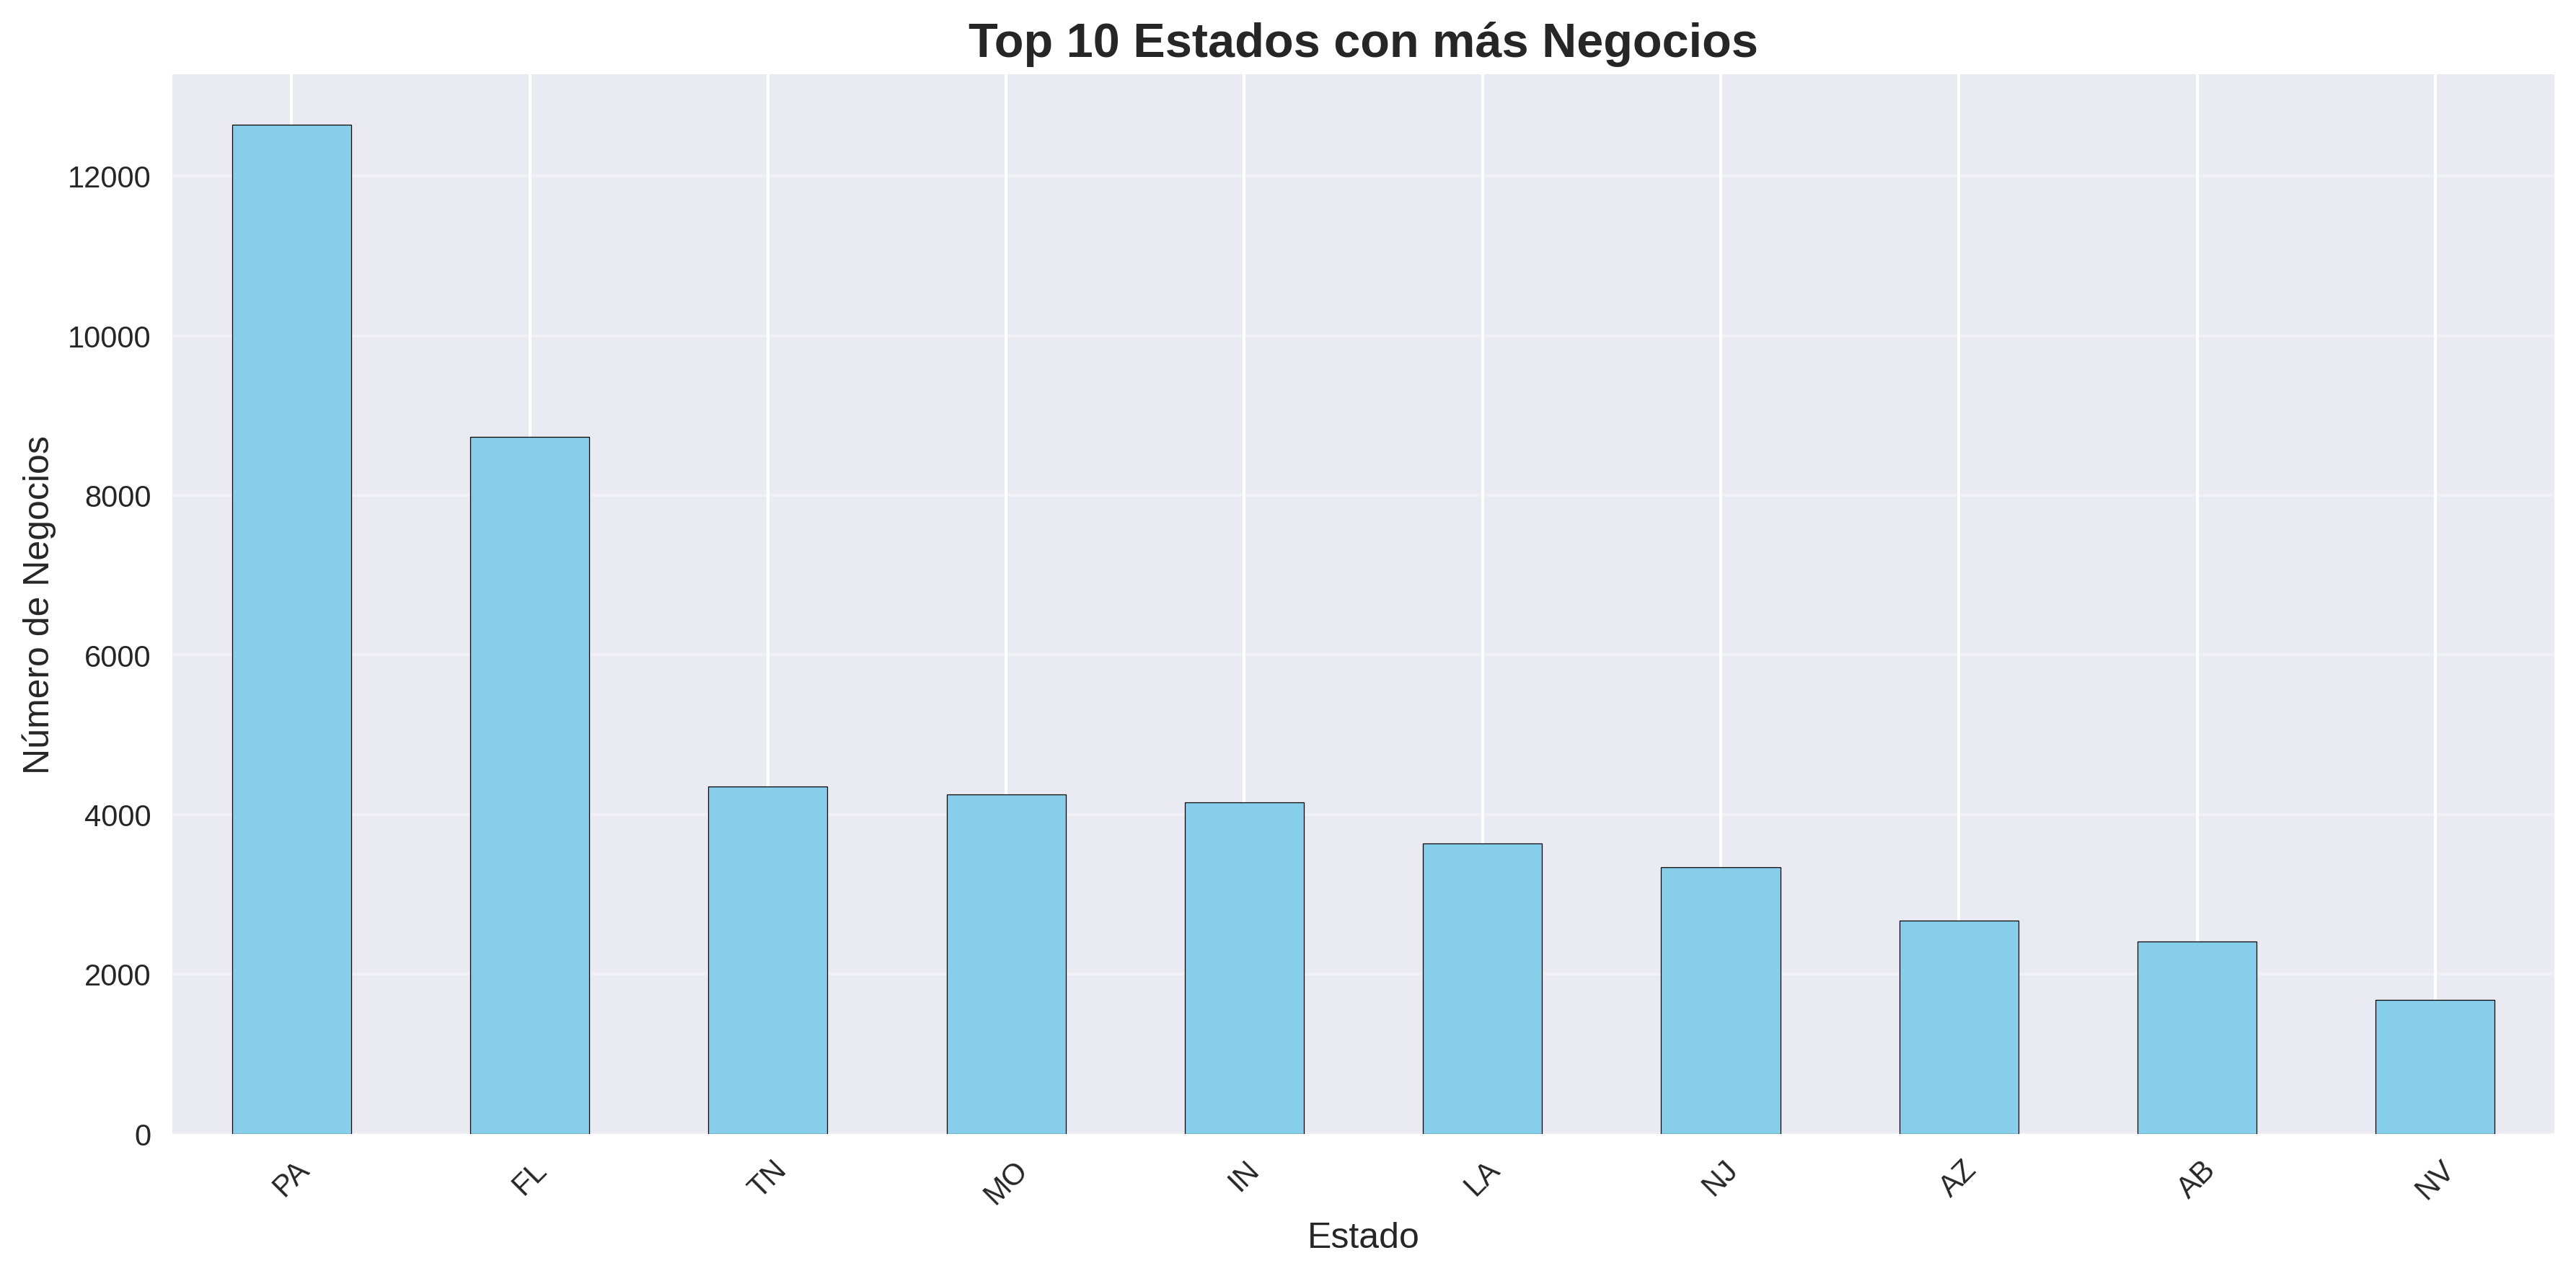
\includegraphics[width=0.8\textwidth]{figures/business_states_distribution.png}
\caption{Distribución de restaurantes por estado}
\label{fig:business_states_distribution}
\end{figure}

\begin{figure}[H]
\centering
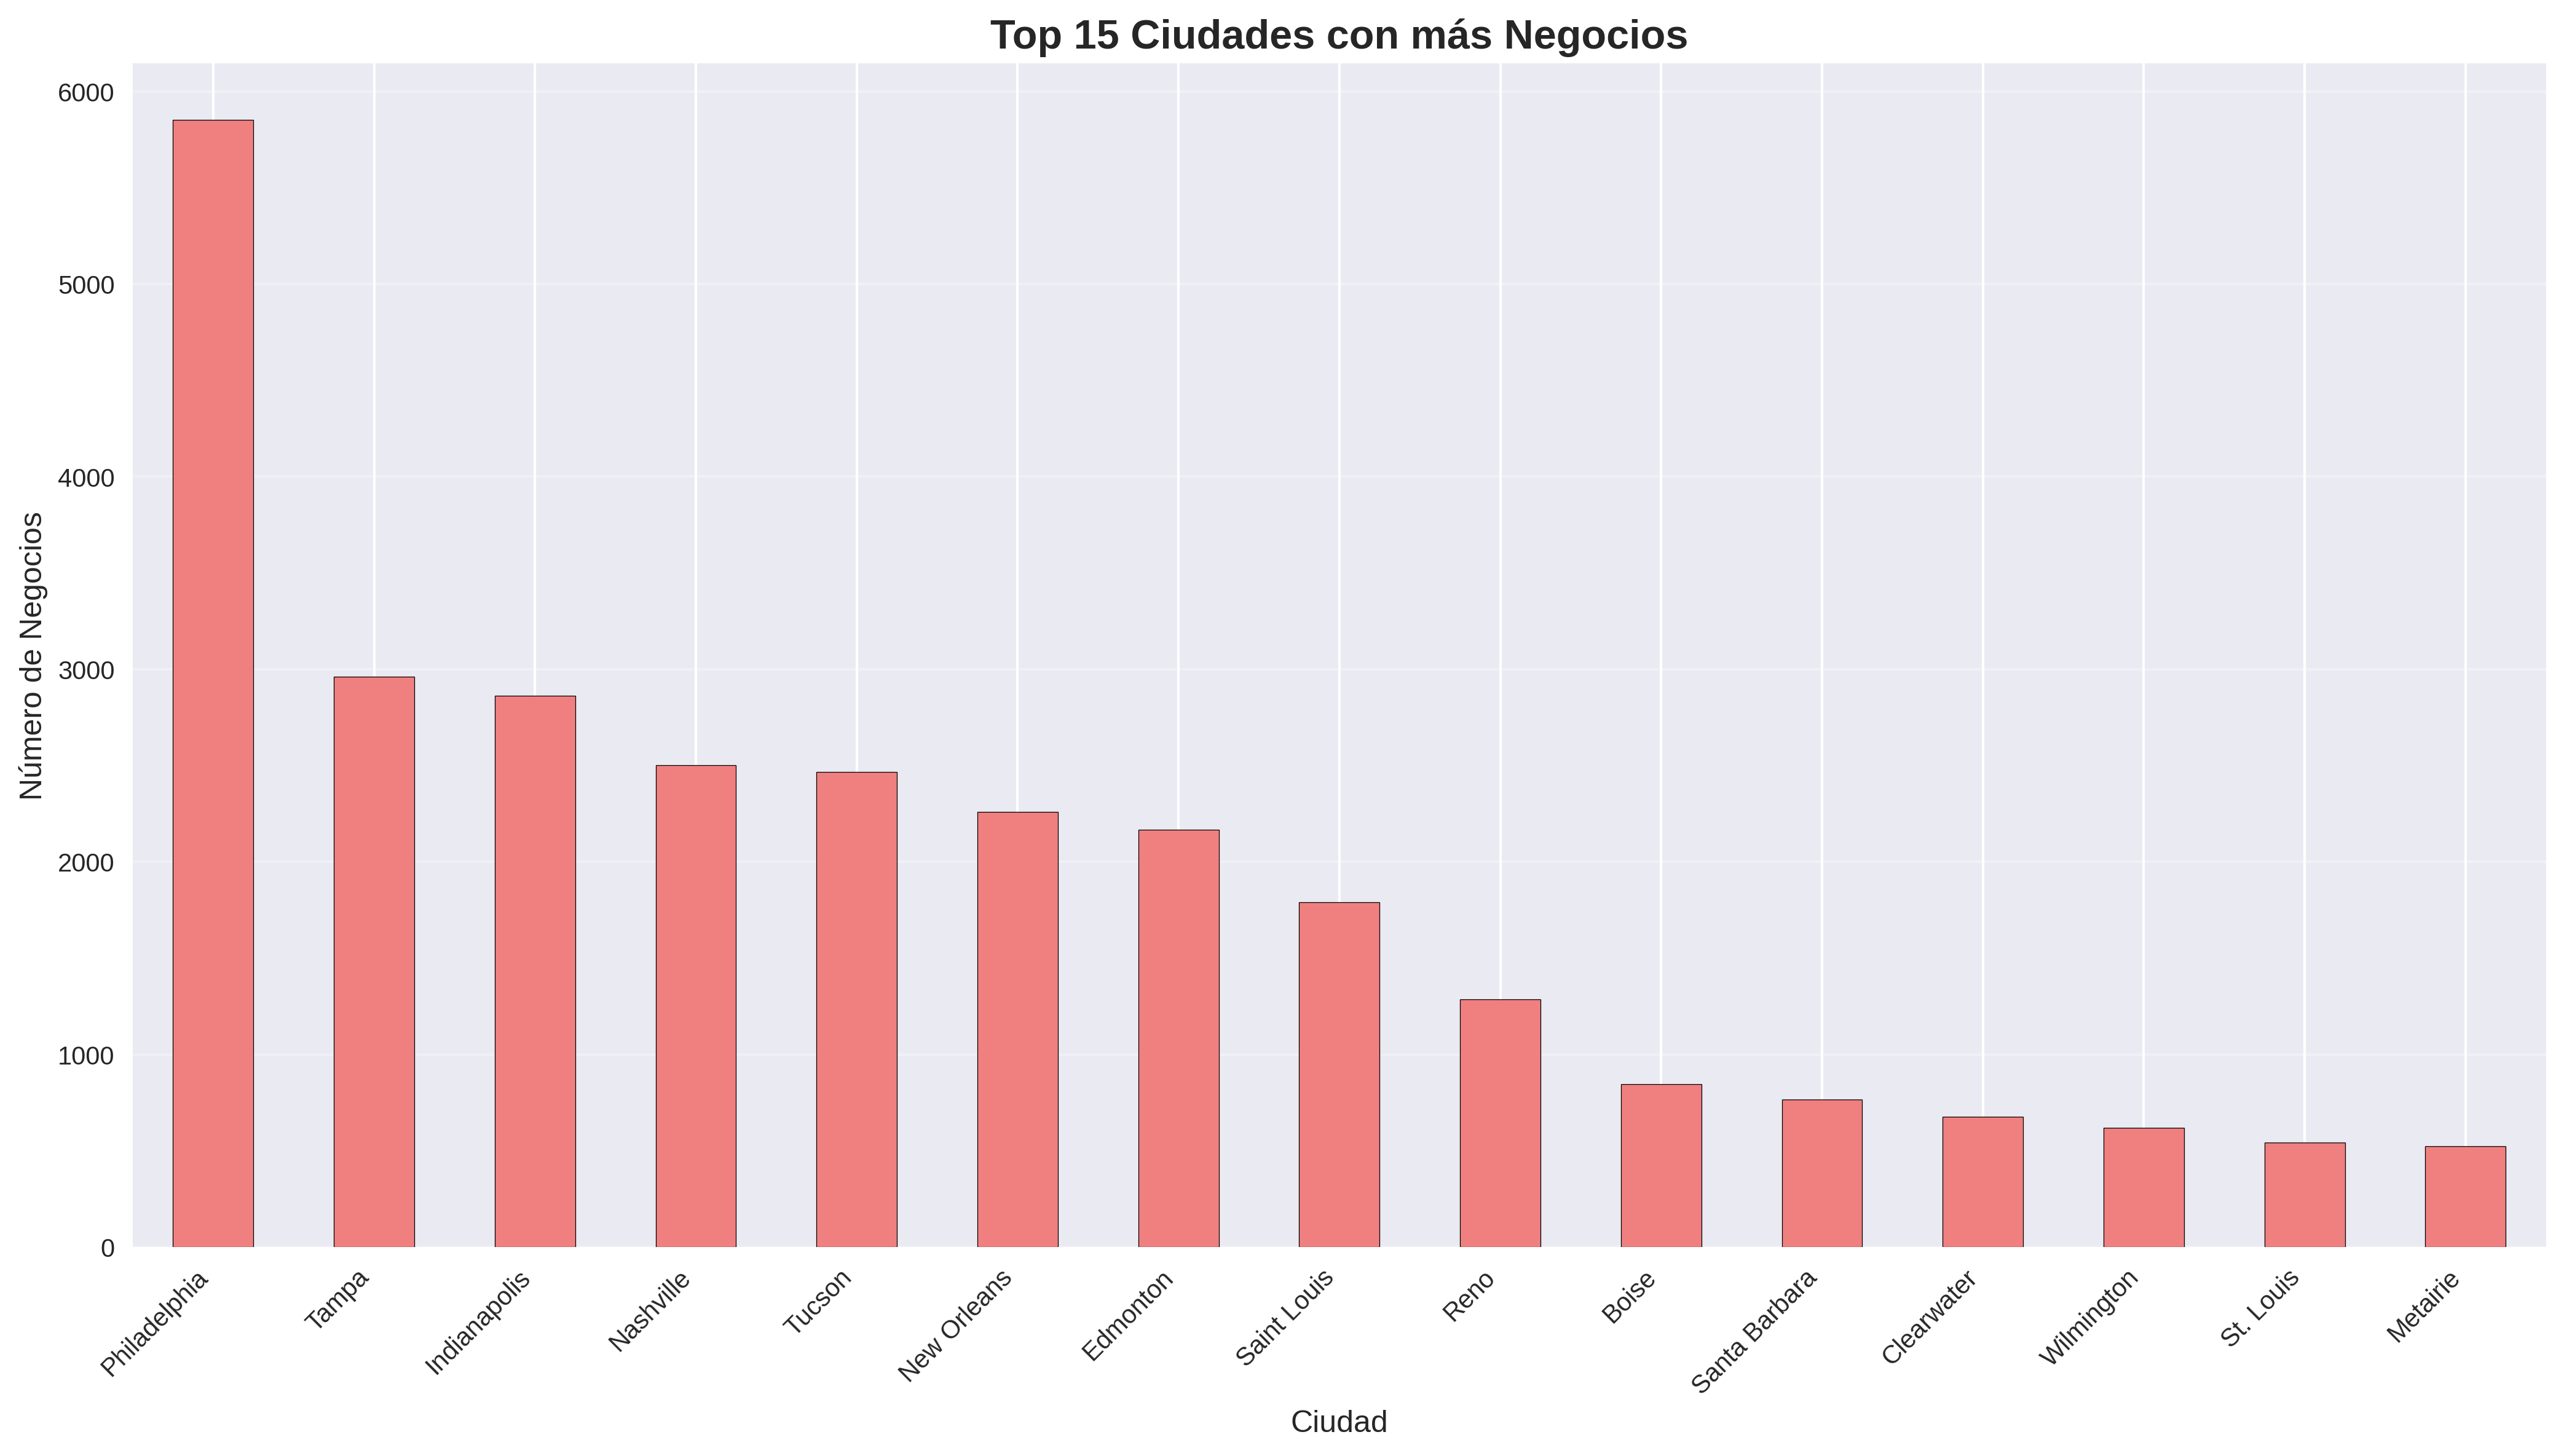
\includegraphics[width=0.8\textwidth]{figures/business_cities_distribution.png}
\caption{Distribución de restaurantes por ciudad (Top 20)}
\label{fig:business_cities_distribution}
\end{figure}

Las Figuras~\ref{fig:business_states_distribution} y~\ref{fig:business_cities_distribution} confirman la concentración geográfica observada en los datos tabulares, mostrando claramente el dominio de Pennsylvania y Florida en el dataset.

\subsection{Estado Operacional}

El análisis del estado operacional mostró una distribución significativa:

\begin{itemize}
    \item \textbf{Restaurantes abiertos}: 34,987 (66.9\%)
    \item \textbf{Restaurantes cerrados}: 17,281 (33.1\%)
    \item \textbf{Ratio operacional}: 2:1 (abiertos vs cerrados)
\end{itemize}

\begin{figure}[H]
\centering
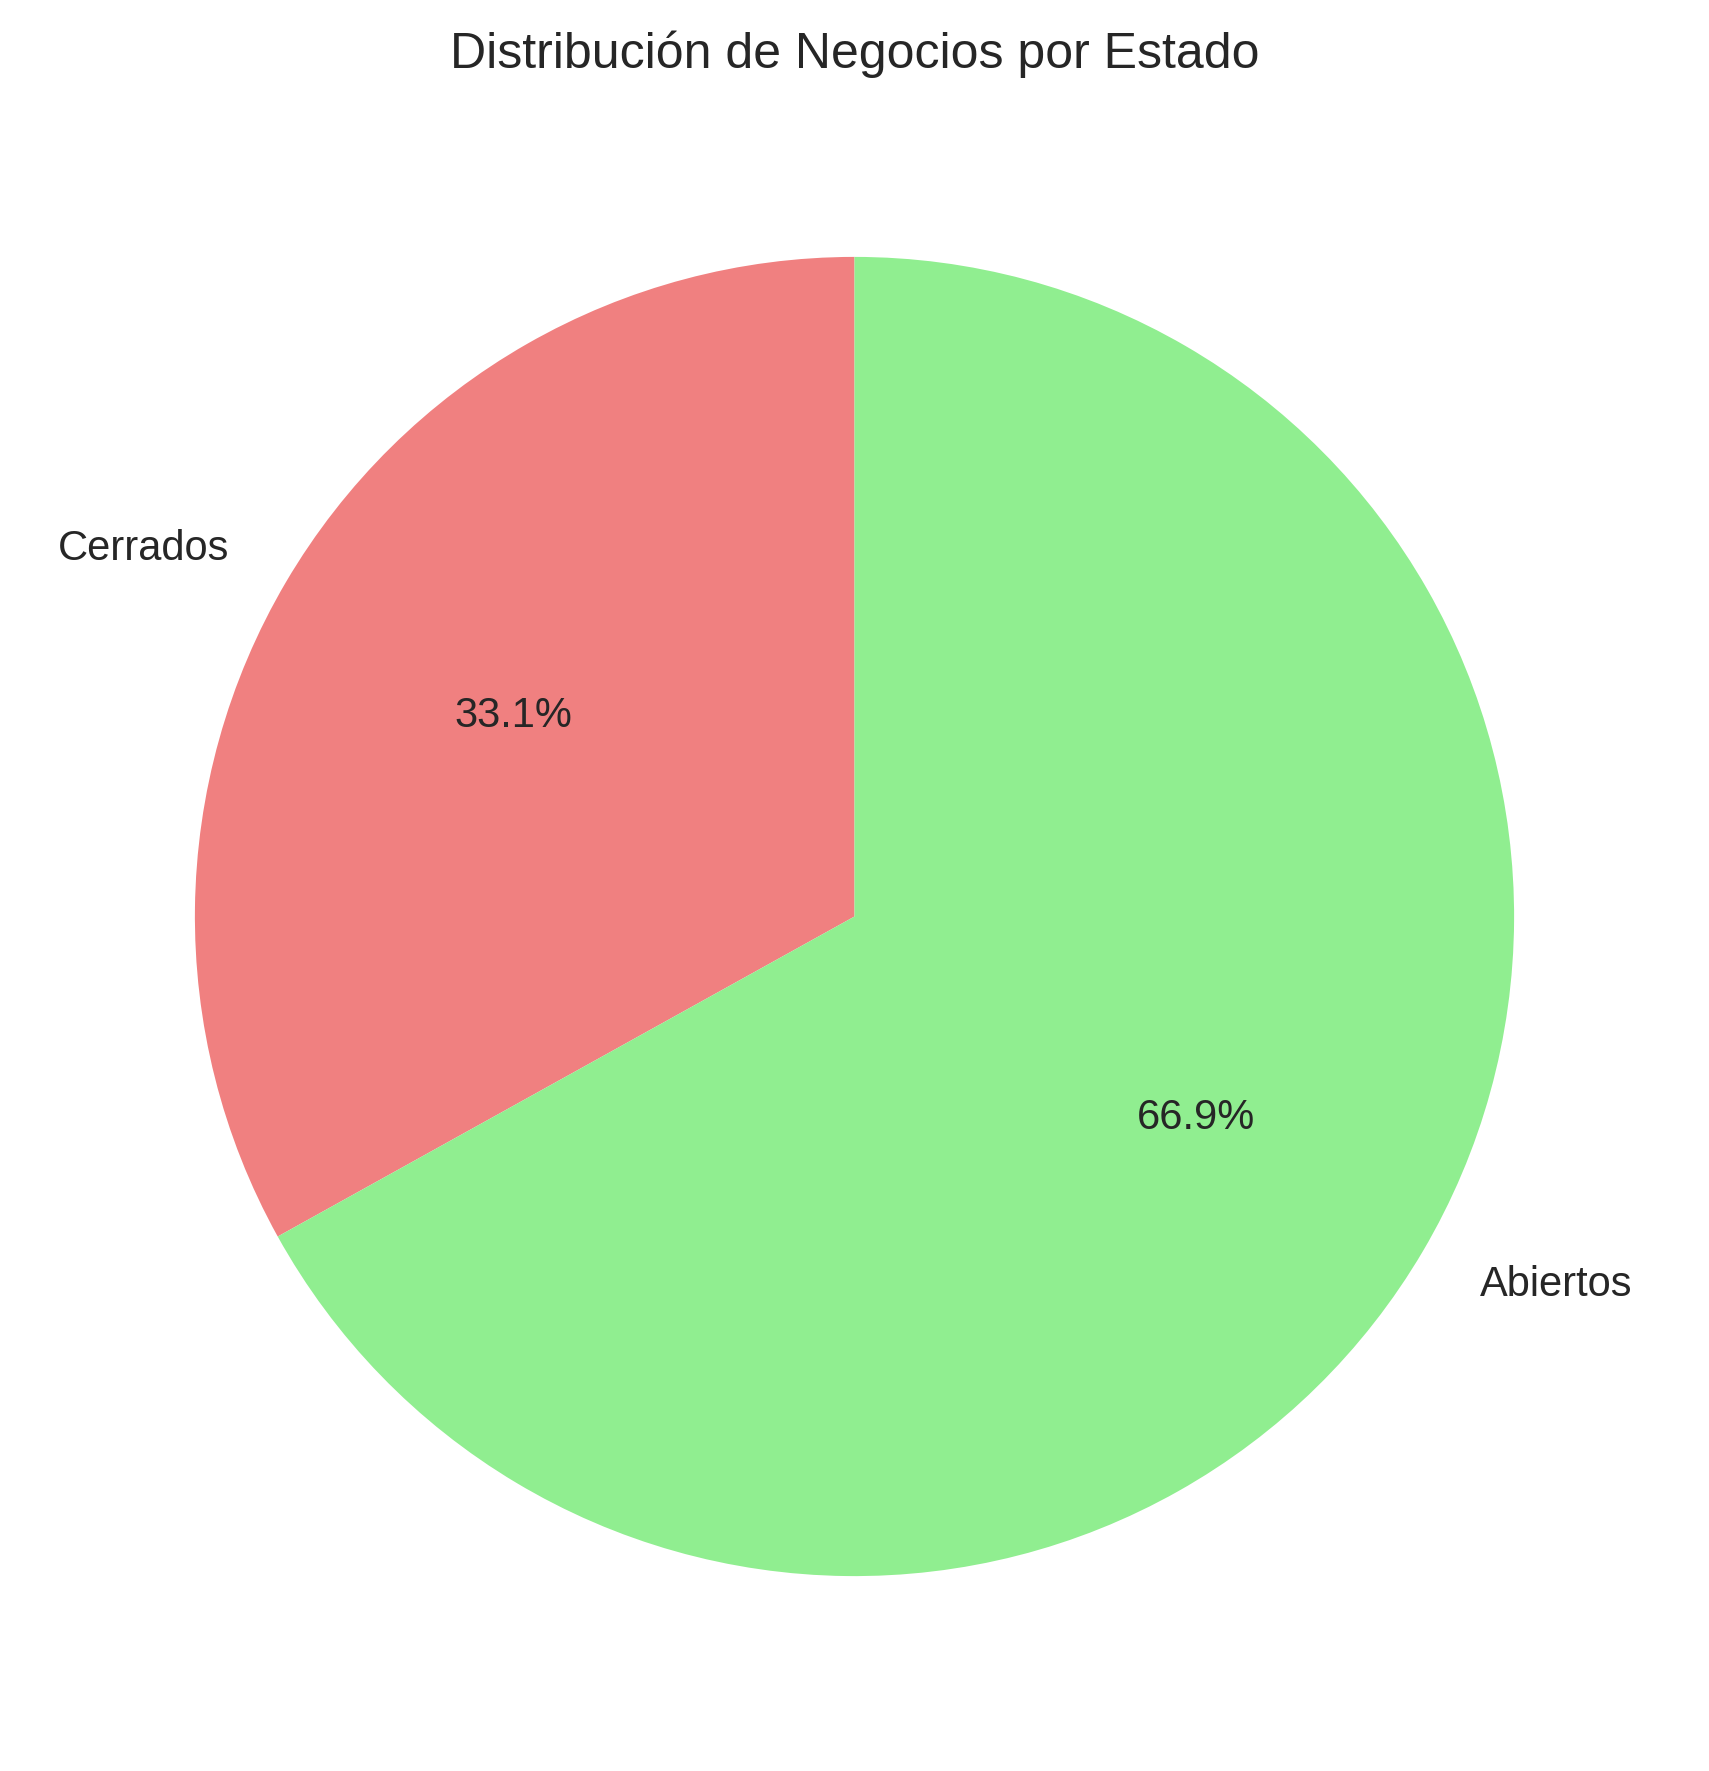
\includegraphics[width=0.6\textwidth]{figures/estado_negocios.png}
\caption{Distribución del estado operacional de restaurantes}
\label{fig:estado_negocios}
\end{figure}

La Figura~\ref{fig:estado_negocios} visualiza la proporción de restaurantes activos versus cerrados, confirmando que aproximadamente dos tercios de los establecimientos en el dataset permanecen operativos.

\subsection{Métricas de Popularidad}

Las métricas de popularidad revelaron patrones interesantes en el engagement de usuarios:

\begin{table}[H]
\centering
\caption{Estadísticas de popularidad de restaurantes}
\begin{tabular}{@{}lr@{}}
\toprule
\textbf{Métrica} & \textbf{Valor} \\
\midrule
Promedio de reseñas por restaurante & 87.27 \\
Mediana de reseñas & 33.00 \\
Máximo de reseñas & 7,568 \\
Mínimo de reseñas (filtrado) & 5 \\
Desviación estándar & 188.94 \\
\bottomrule
\end{tabular}
\end{table}

Los restaurantes más reseñados incluyen:
\begin{enumerate}
    \item \textbf{Acme Oyster House} (New Orleans, LA) - 7,568 reseñas, 4.0 estrellas
    \item \textbf{Oceana Grill} (New Orleans, LA) - 7,400 reseñas, 4.0 estrellas
    \item \textbf{Hattie B's Hot Chicken} (Nashville, TN) - 6,093 reseñas, 4.5 estrellas
    \item \textbf{Reading Terminal Market} (Philadelphia, PA) - 5,721 reseñas, 4.5 estrellas
\end{enumerate}

\begin{figure}[H]
\centering
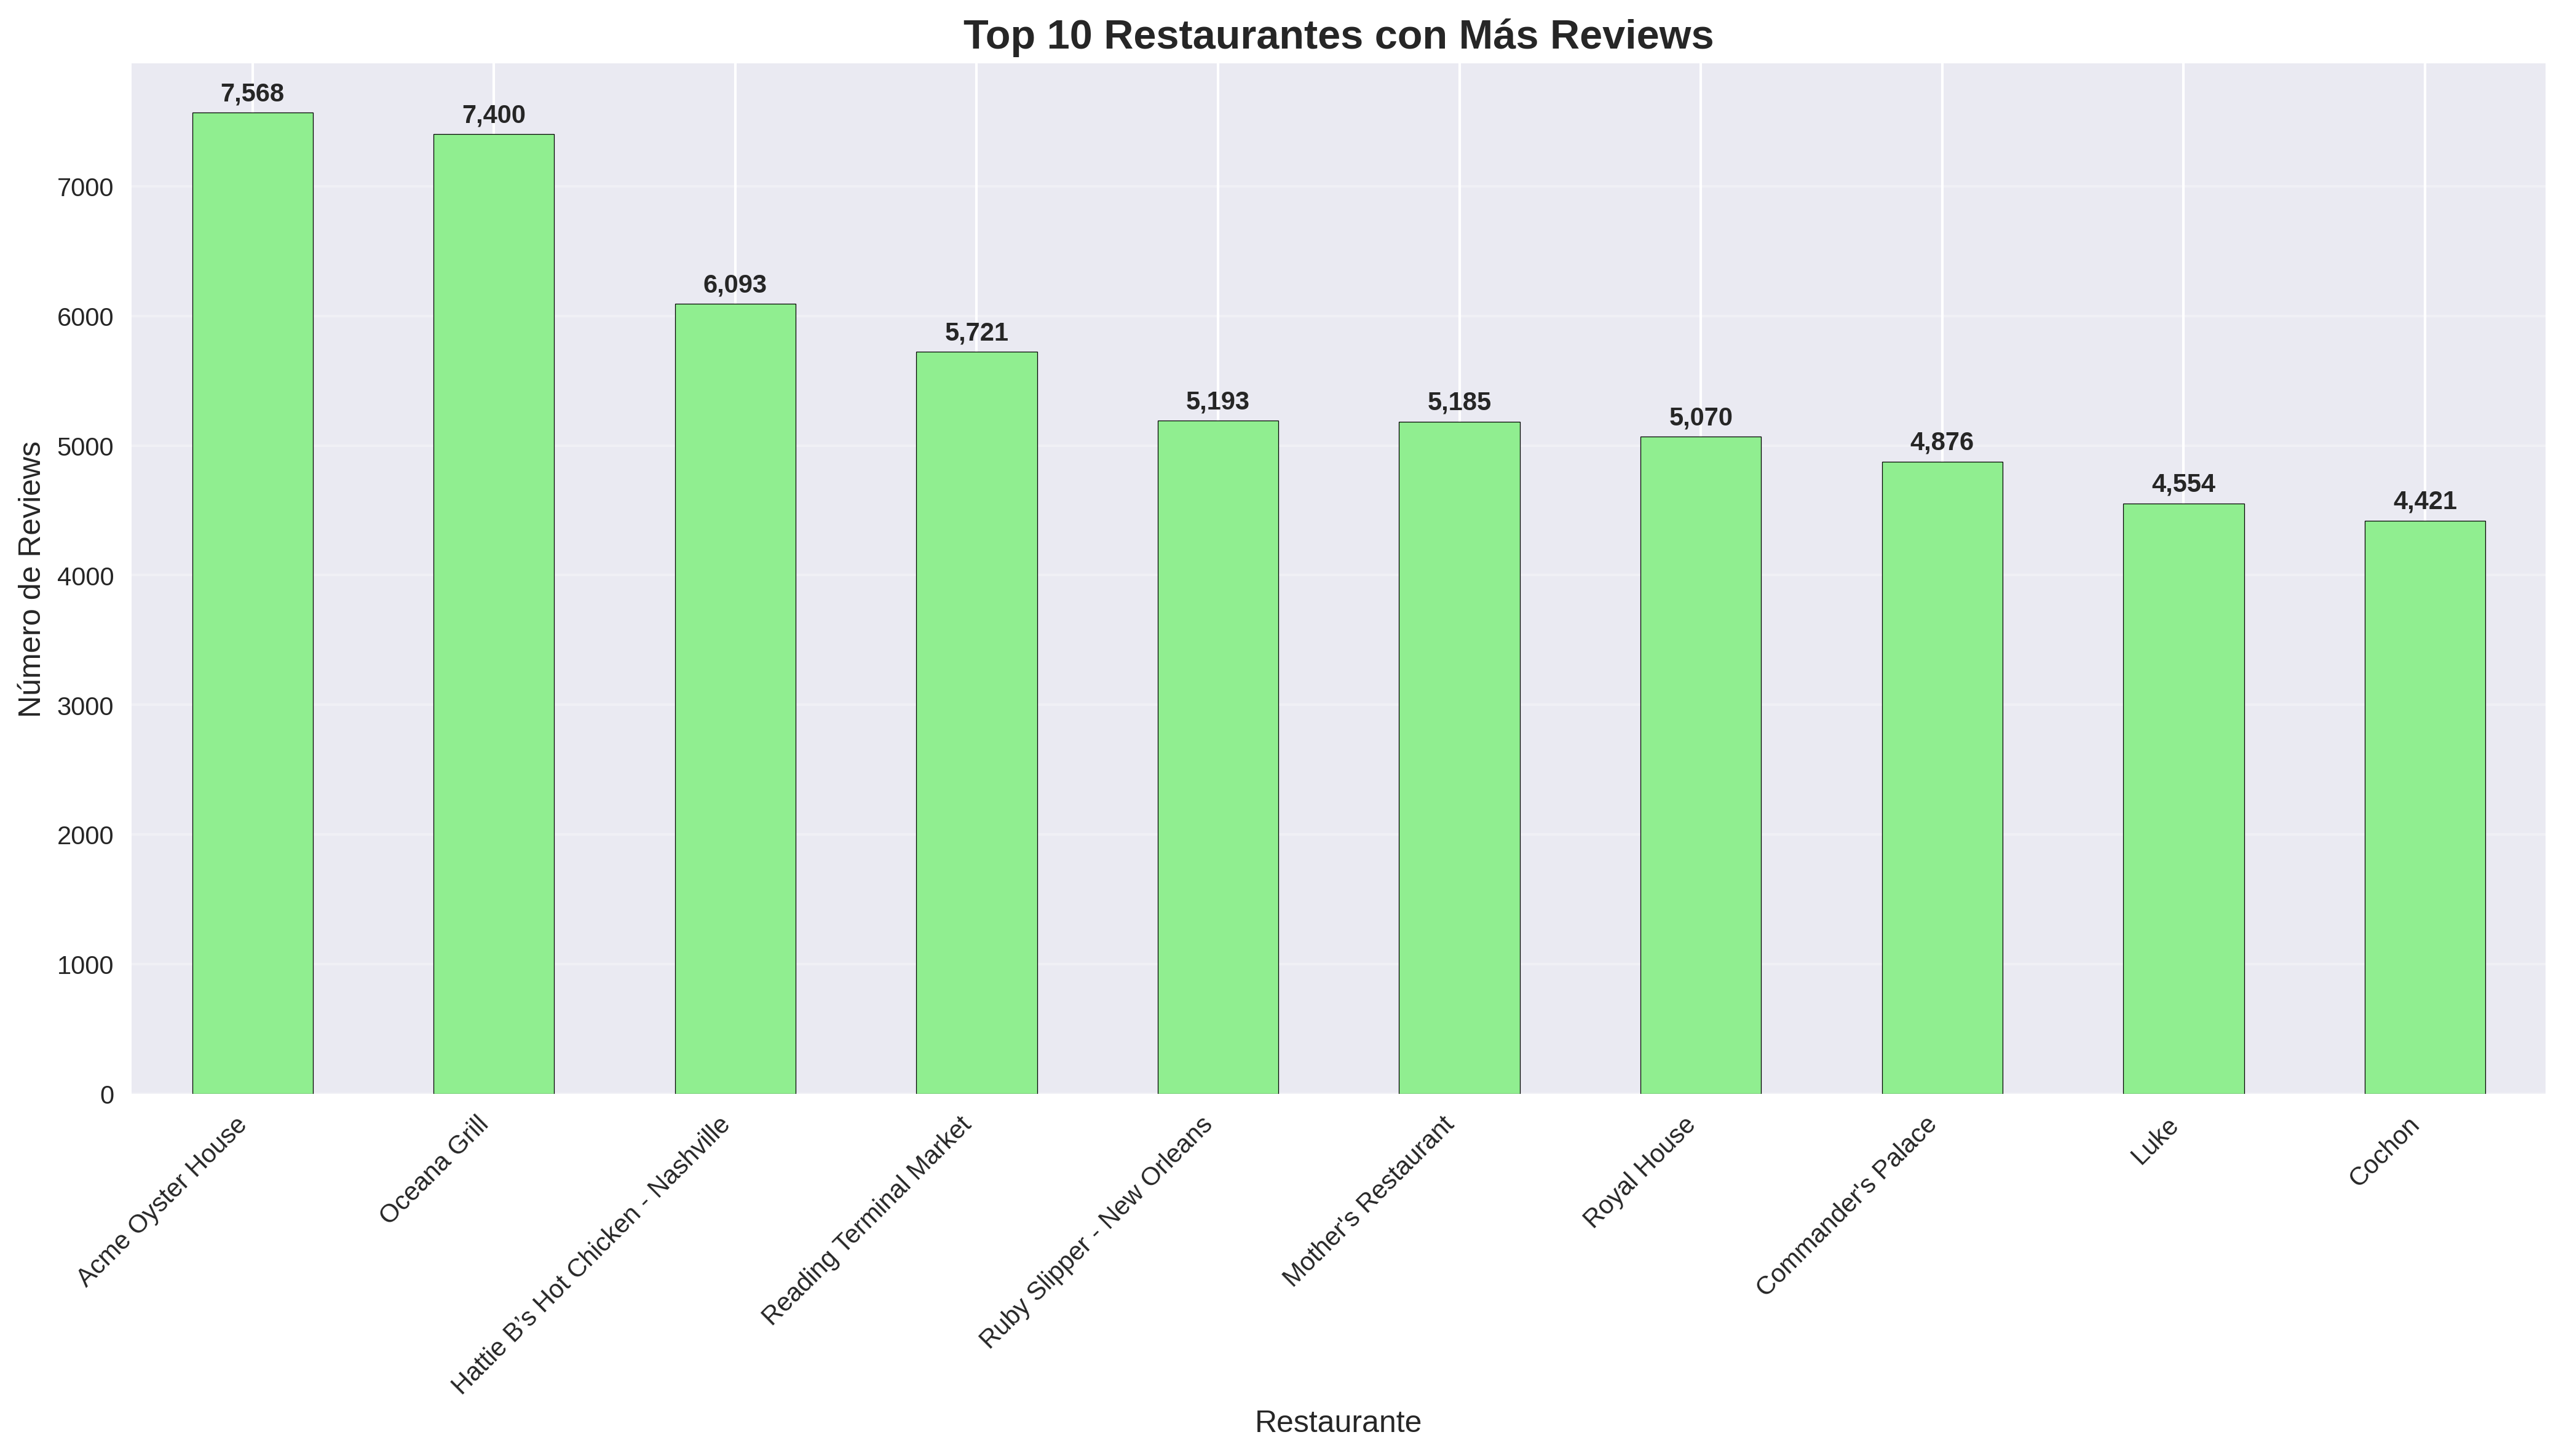
\includegraphics[width=0.9\textwidth]{figures/business_top_restaurants_by_reviews.png}
\caption{Top 20 restaurantes por número de reseñas}
\label{fig:business_top_restaurants}
\end{figure}

La Figura~\ref{fig:business_top_restaurants} muestra los restaurantes con mayor engagement de usuarios, destacando establecimientos icónicos de ciudades como New Orleans, Nashville y Philadelphia.

\subsection{Distribución de Calificaciones}

El análisis de calificaciones mostró tendencias optimistas en el sector:

\begin{table}[H]
\centering
\caption{Estadísticas de calificaciones de restaurantes}
\begin{tabular}{@{}lr@{}}
\toprule
\textbf{Métrica} & \textbf{Valor} \\
\midrule
Promedio general & 3.52 estrellas \\
Mediana & 3.50 estrellas \\
Calificación más común & 4.0 estrellas (25.7\%) \\
Restaurantes con 4+ estrellas & 23,348 (44.7\%) \\
\bottomrule
\end{tabular}
\end{table}

\begin{figure}[H]
\centering
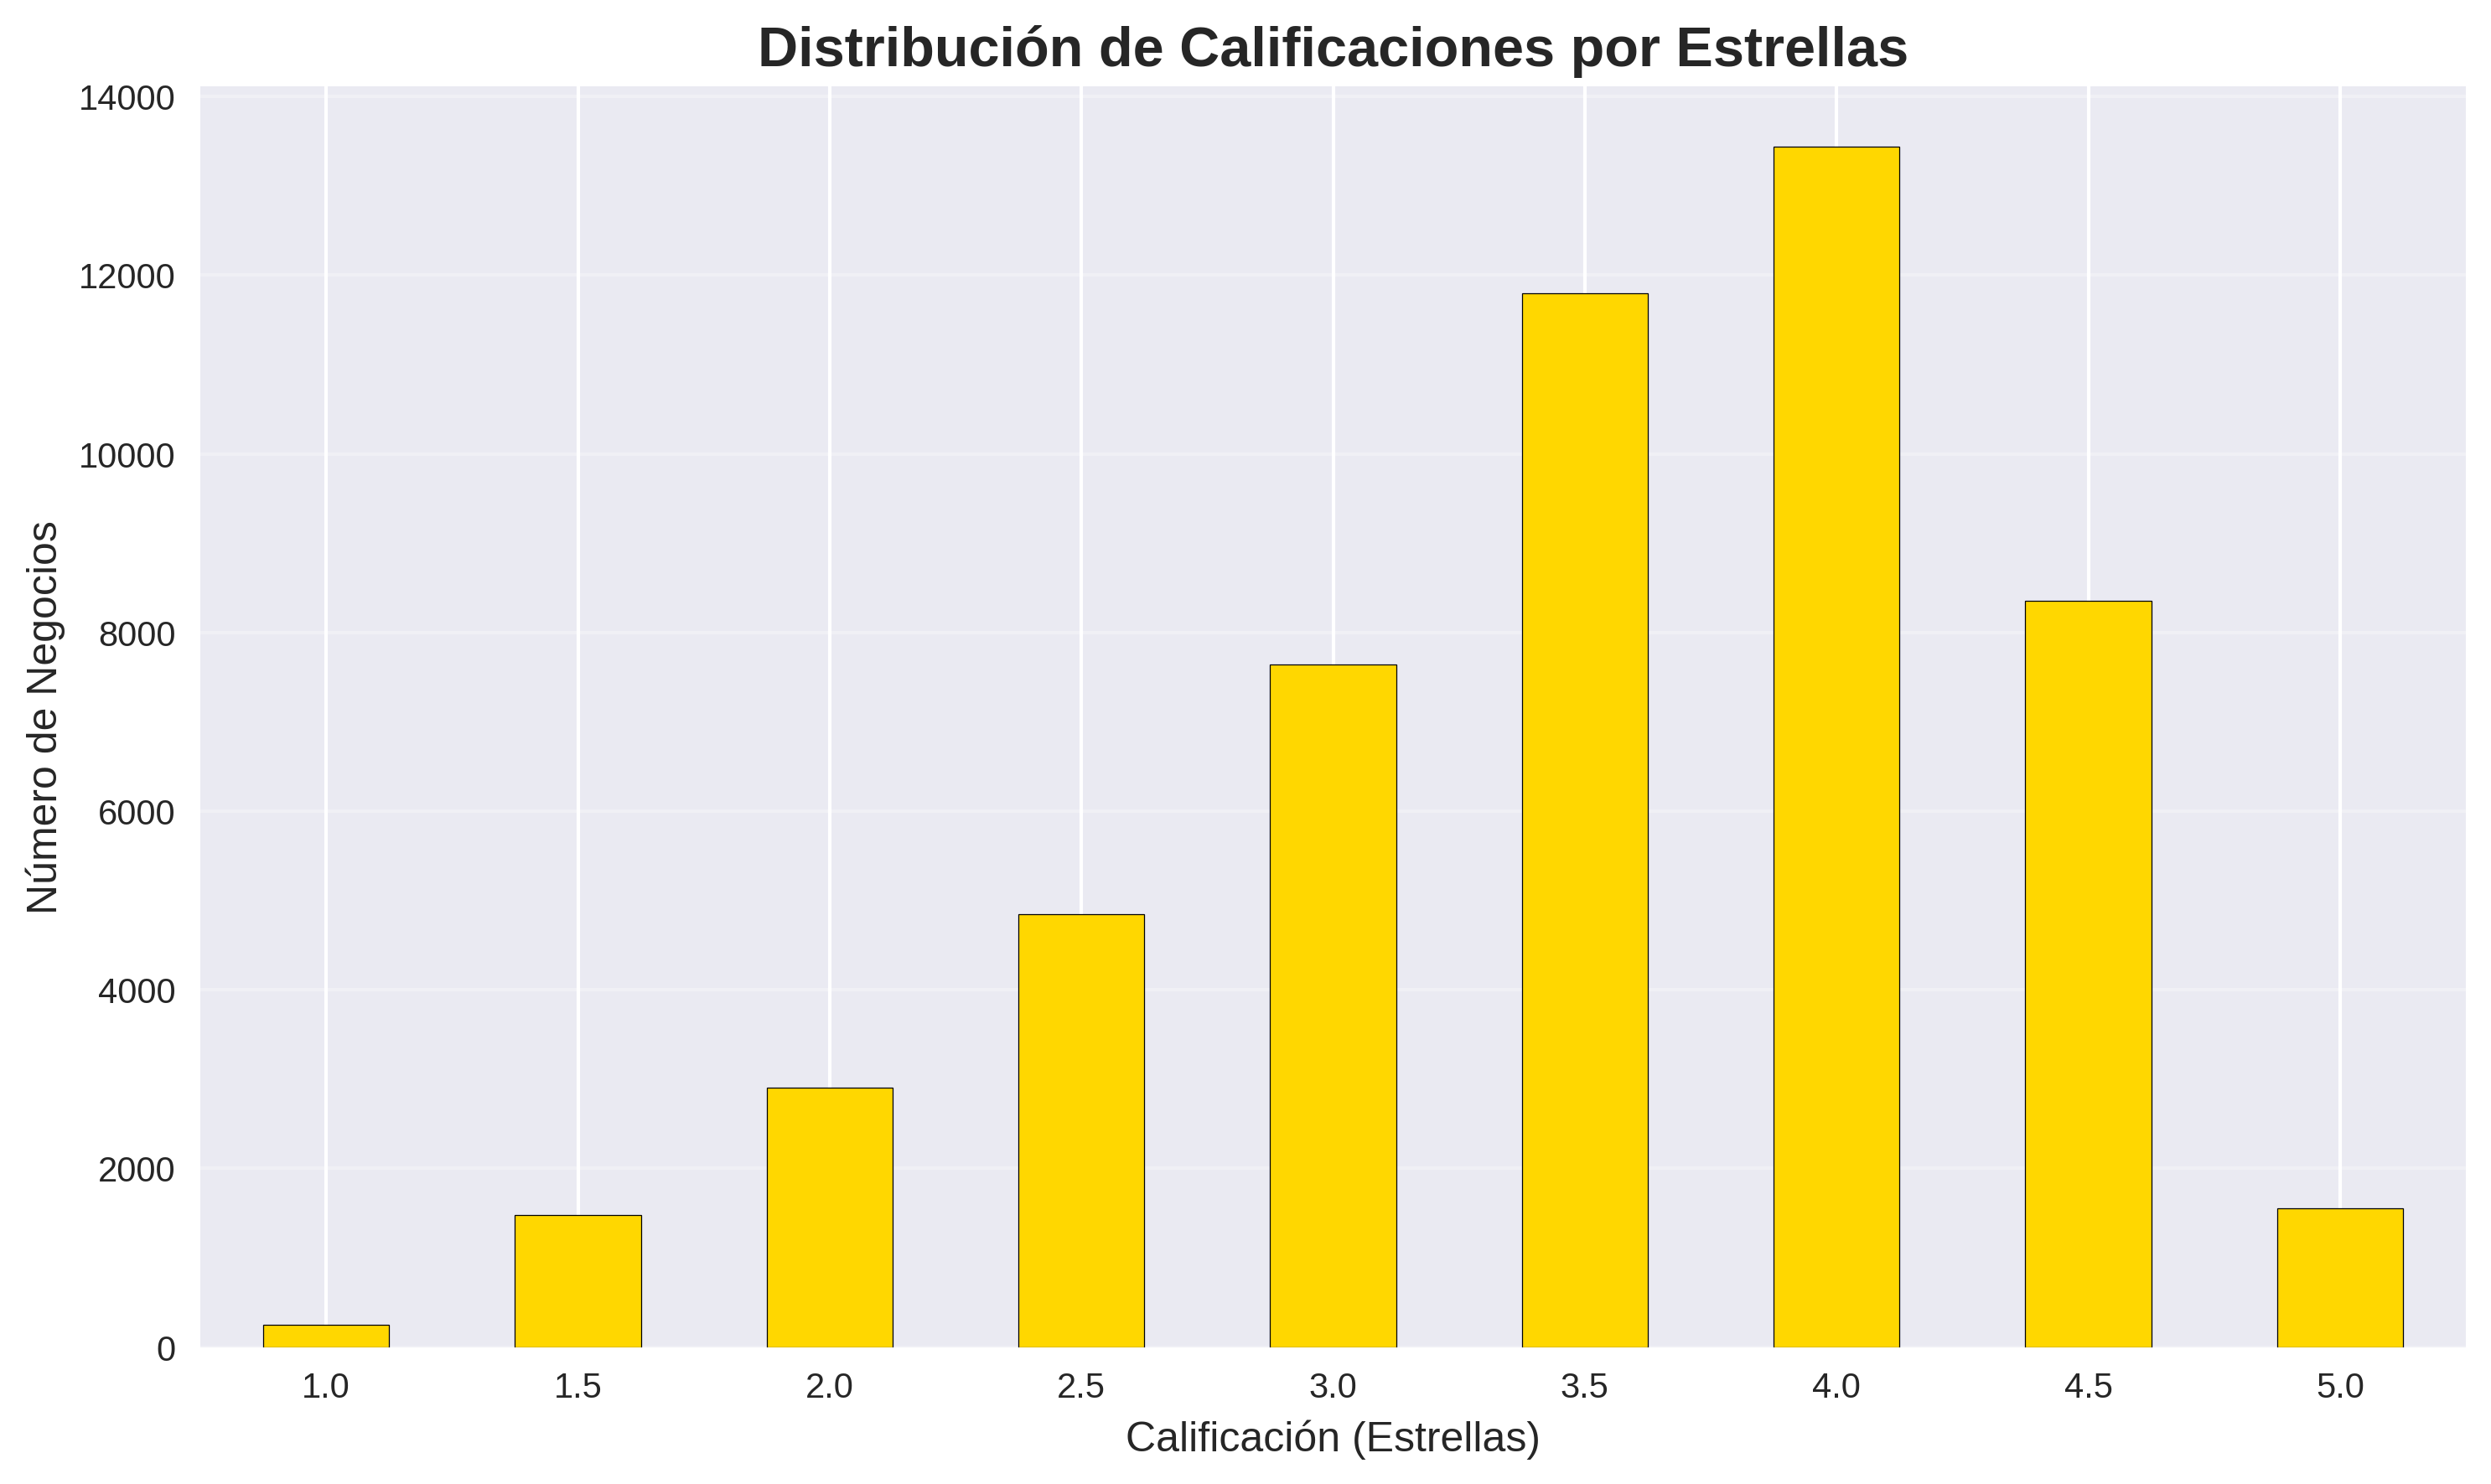
\includegraphics[width=0.7\textwidth]{figures/business_ratings_distribution.png}
\caption{Distribución de calificaciones de restaurantes}
\label{fig:business_ratings_distribution}
\end{figure}

La Figura~\ref{fig:business_ratings_distribution} confirma la tendencia positiva en las calificaciones, con una distribución sesgada hacia calificaciones altas, indicando un nivel general satisfactorio en la experiencia gastronómica.

\subsection{Categorías de Restaurantes}

El análisis de categorías reveló la diversidad del sector gastronómico:

\begin{table}[H]
\centering
\caption{Principales categorías de restaurantes}
\begin{tabular}{@{}lrr@{}}
\toprule
\textbf{Categoría} & \textbf{Negocios} & \textbf{Porcentaje} \\
\midrule
Restaurants & 52,268 & 100.0\% \\
Food & 15,472 & 29.6\% \\
Nightlife & 8,723 & 16.7\% \\
Sandwiches & 8,366 & 16.0\% \\
Bars & 8,337 & 16.0\% \\
\bottomrule
\end{tabular}
\end{table}

\begin{figure}[H]
\centering
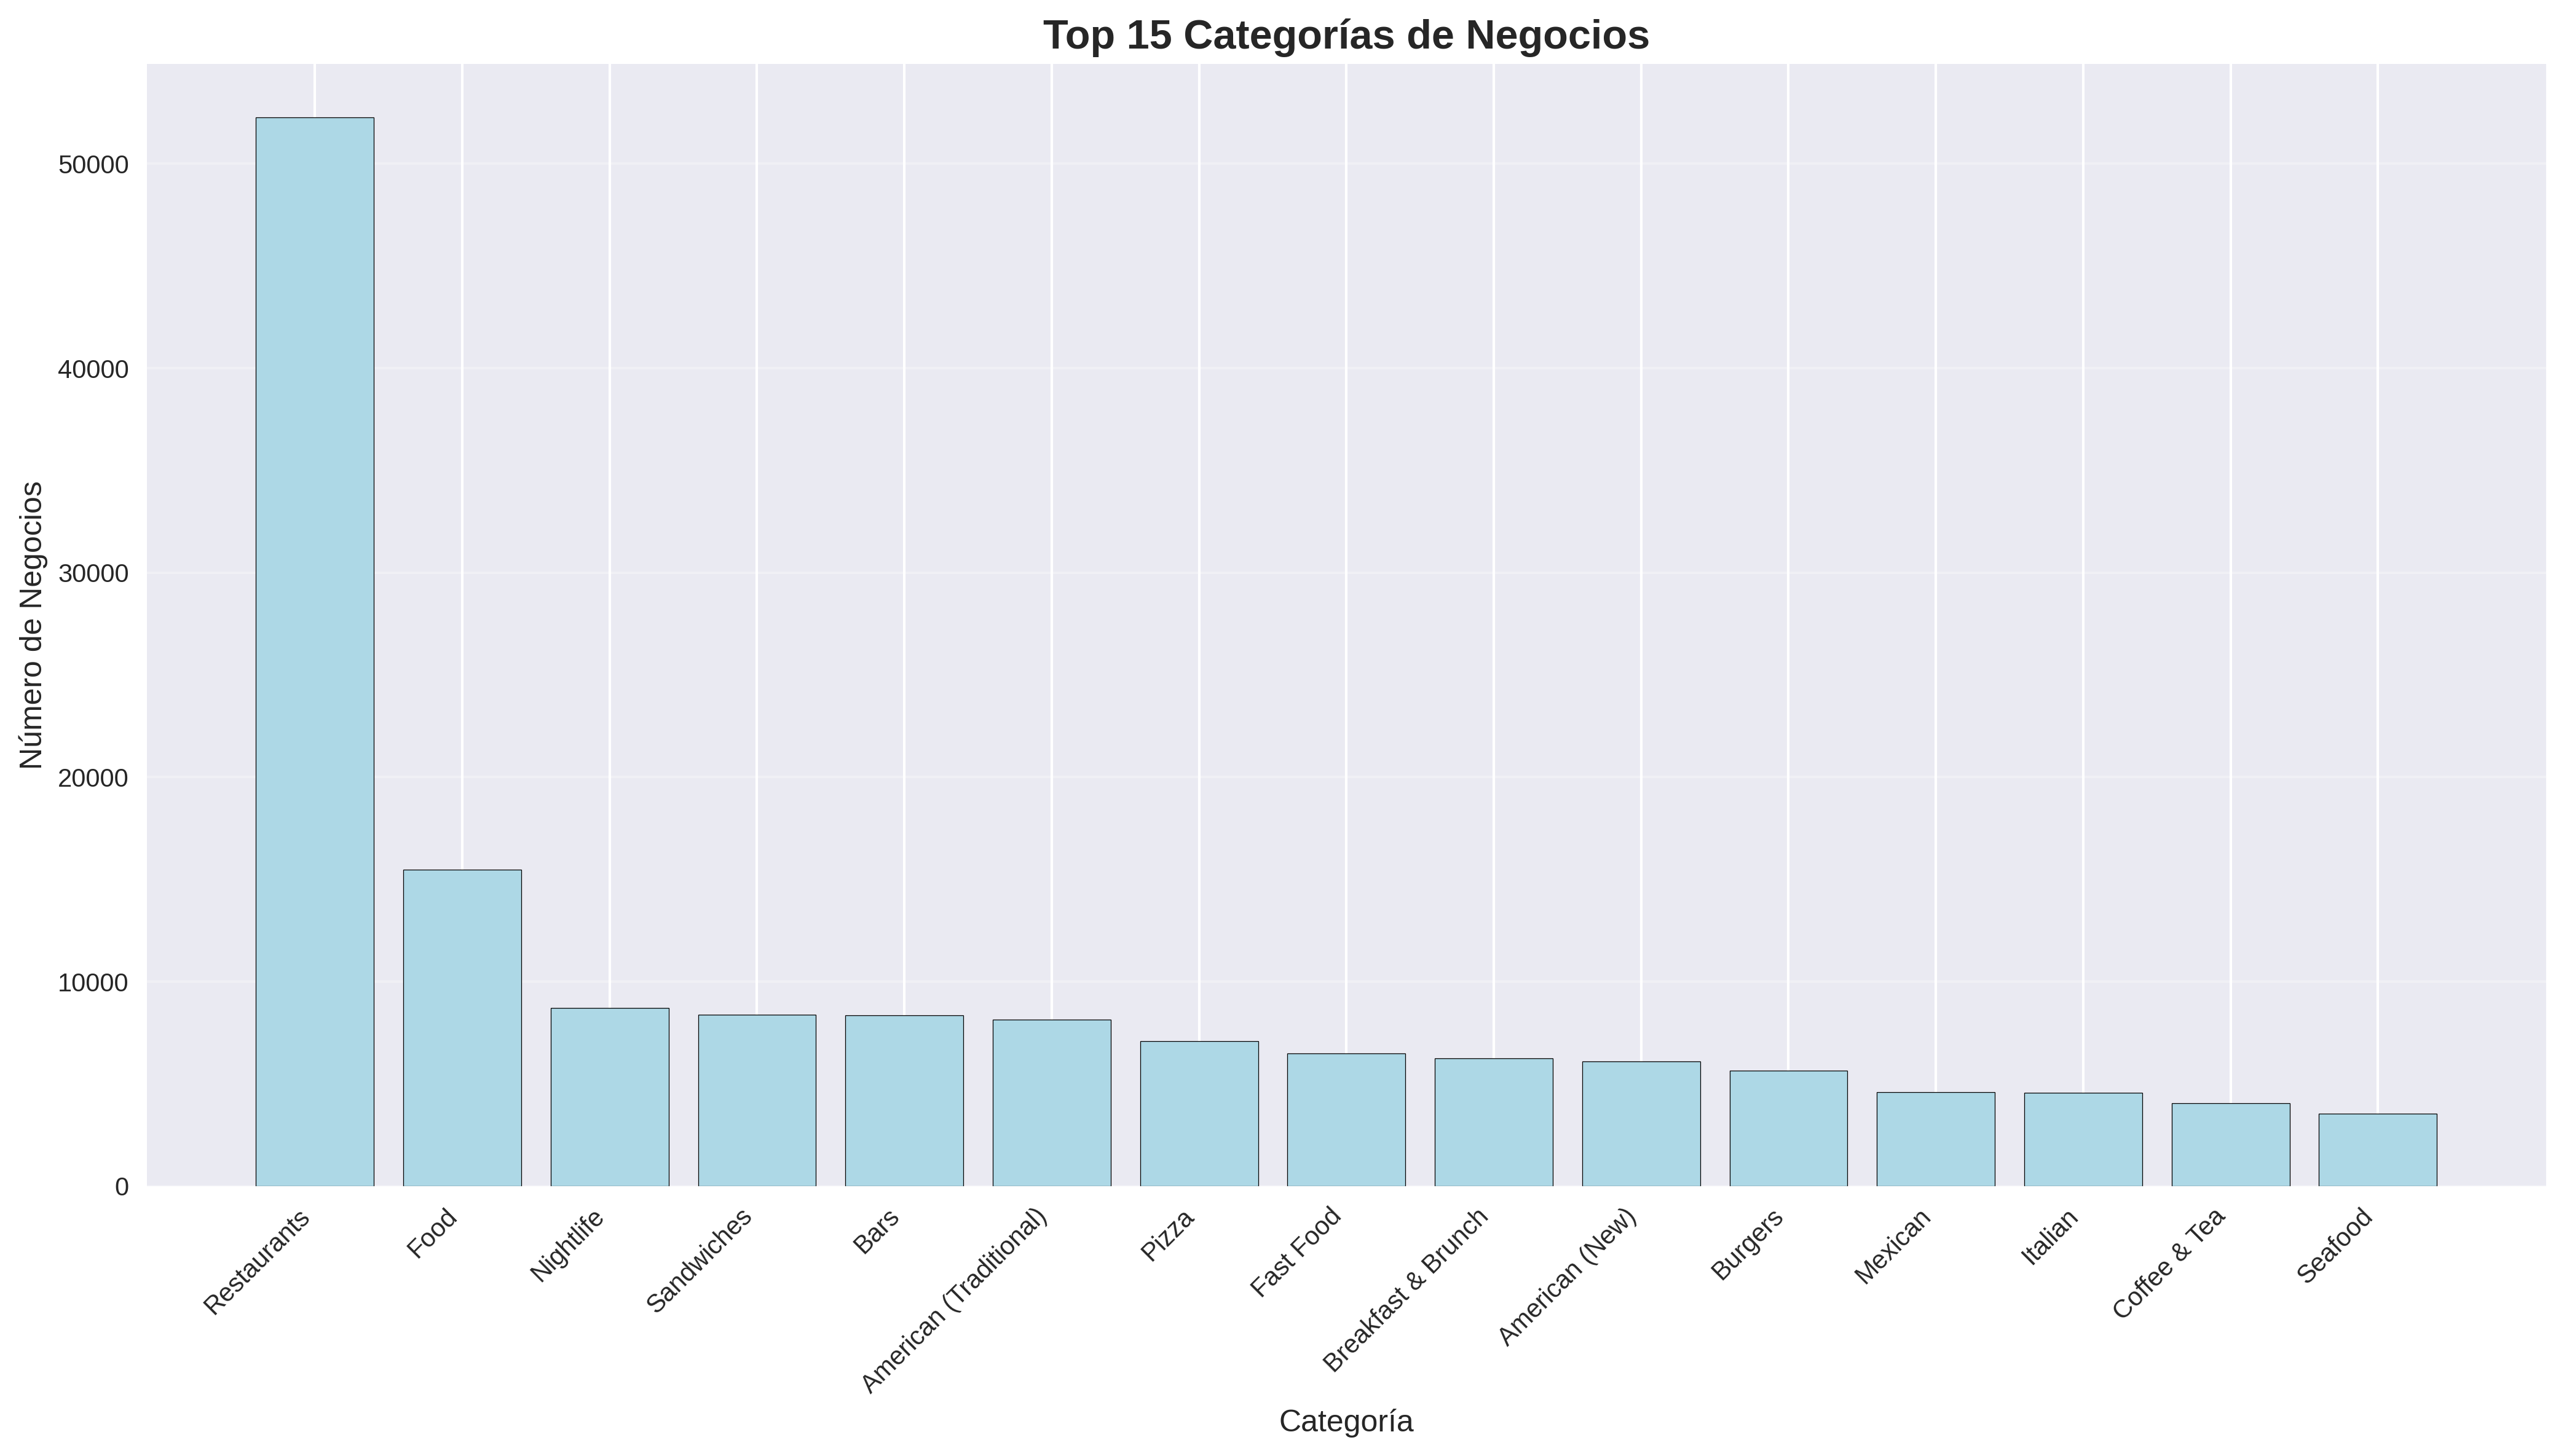
\includegraphics[width=0.8\textwidth]{figures/business_top_categories.png}
\caption{Top 20 categorías de negocios gastronómicos}
\label{fig:business_top_categories}
\end{figure}

La Figura~\ref{fig:business_top_categories} ilustra la diversidad de categorías gastronómicas en el dataset, desde restaurantes tradicionales hasta bares, establecimientos de comida rápida y experiencias culinarias especializadas.

\section{Análisis de Reseñas y Usuarios}

\subsection{Distribución de Calificaciones en Reseñas}

El análisis de reseñas individuales mostró patrones de comportamiento distintos a las calificaciones agregadas:

\begin{table}[H]
\centering
\caption{Estadísticas de calificaciones en reseñas}
\begin{tabular}{@{}lr@{}}
\toprule
\textbf{Métrica} & \textbf{Valor} \\
\midrule
Promedio general & 3.794 estrellas \\
Mediana & 4.0 estrellas \\
Moda & 5.0 estrellas \\
Desviación estándar & 1.391 \\
Sesgo & -0.889 (negativo) \\
\bottomrule
\end{tabular}
\end{table}

La distribución detallada muestra:
\begin{itemize}
    \item \textbf{5 estrellas}: 2,079,441 reseñas (44.01\%)
    \item \textbf{4 estrellas}: 1,130,251 reseñas (23.92\%)
    \item \textbf{3 estrellas}: 543,108 reseñas (11.50\%)
    \item \textbf{2 estrellas}: 404,486 reseñas (8.56\%)
    \item \textbf{1 estrella}: 567,185 reseñas (12.01\%)
\end{itemize}

\begin{figure}[H]
\centering
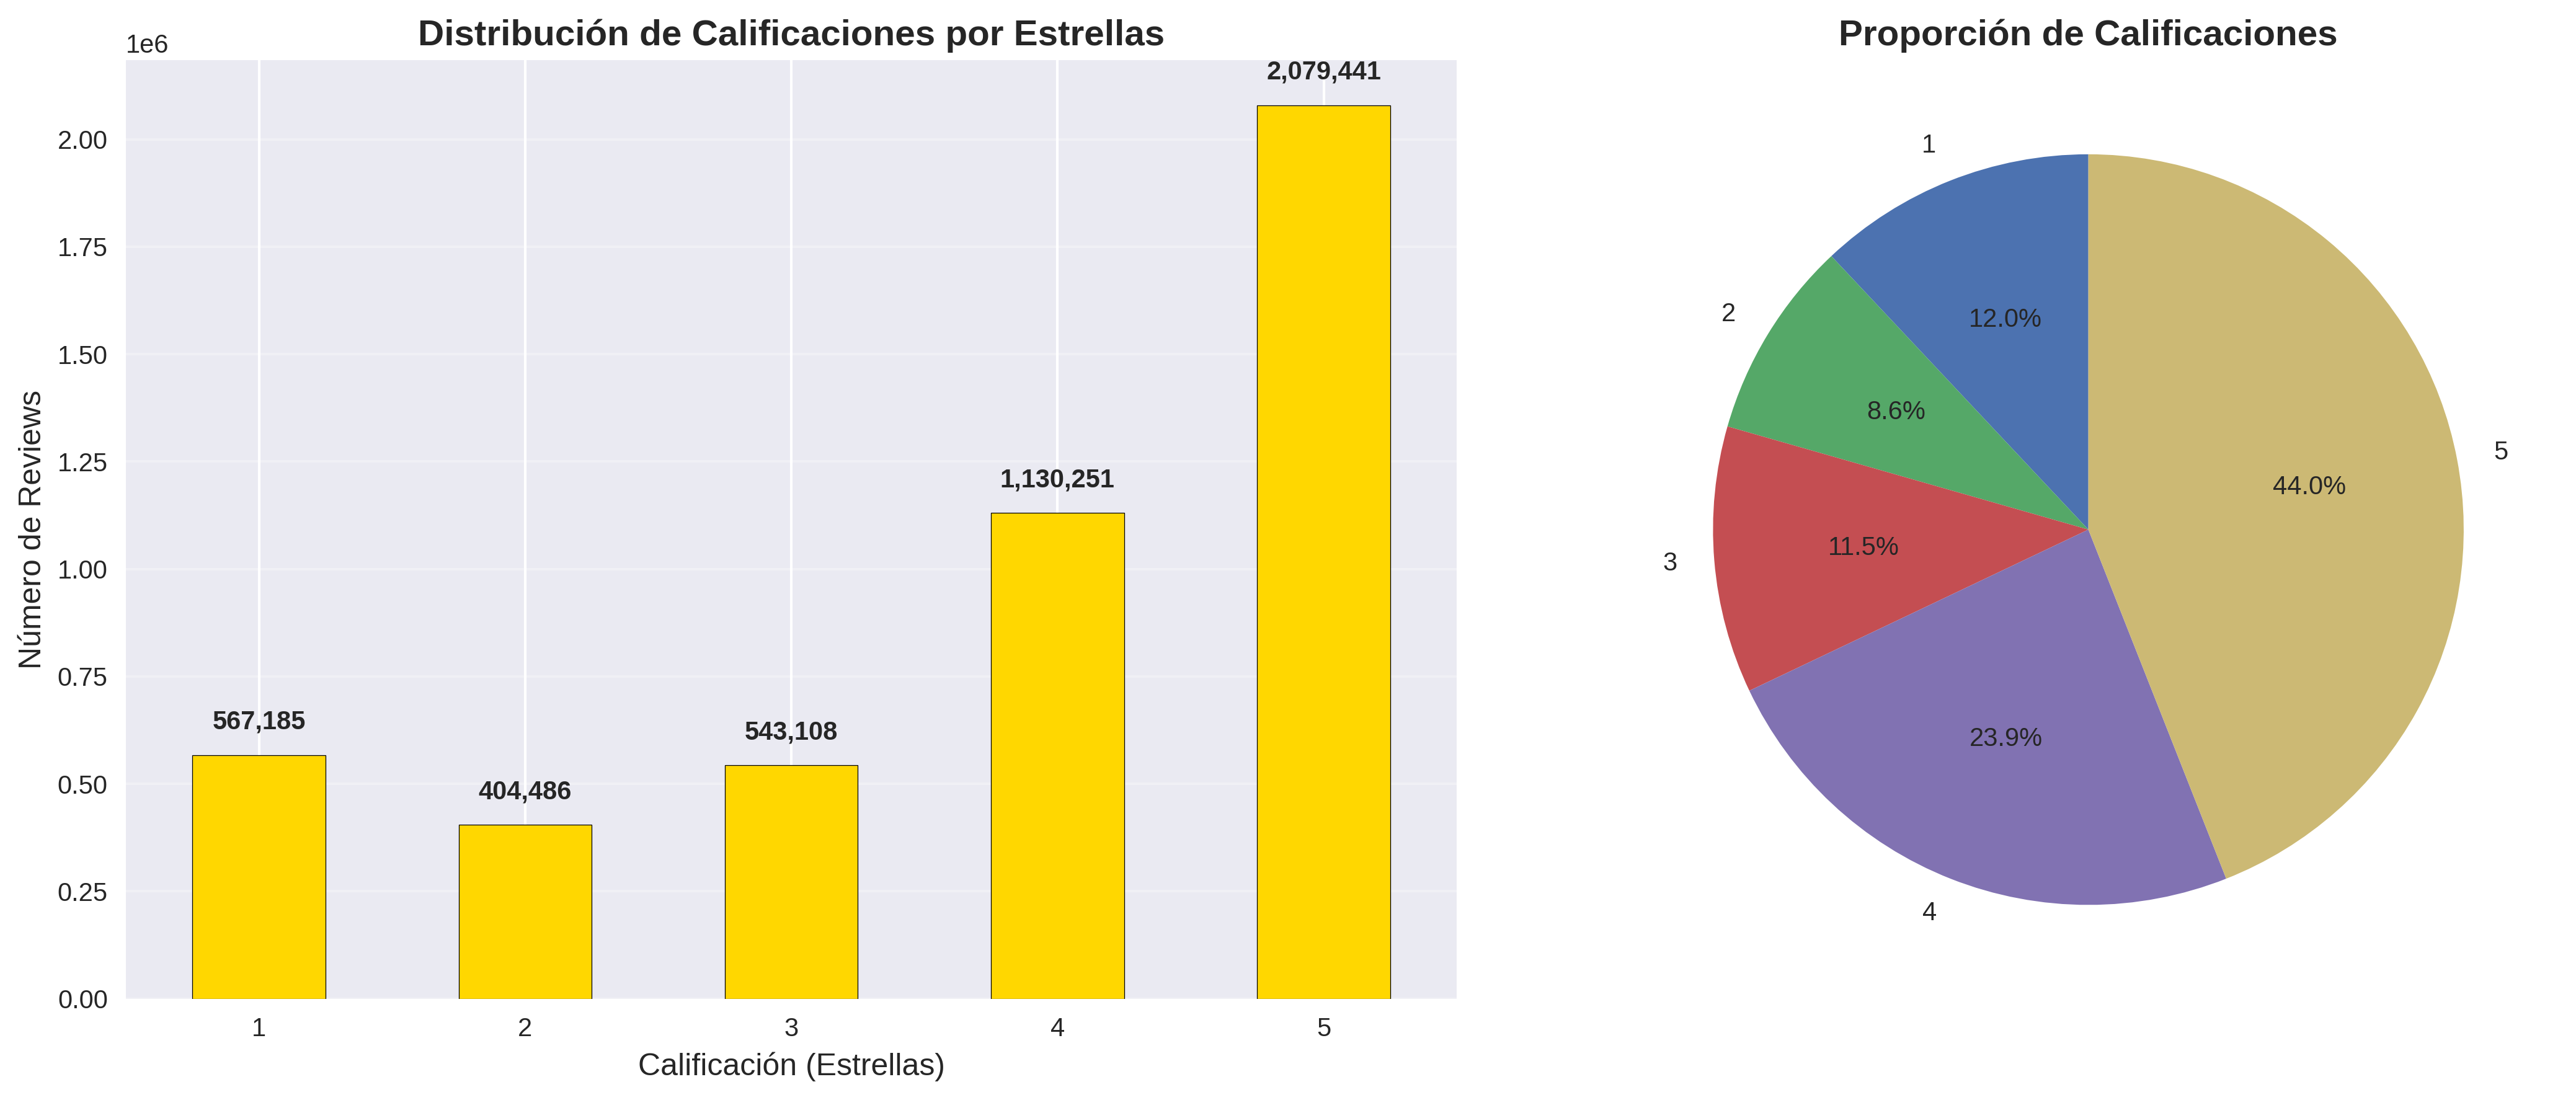
\includegraphics[width=0.7\textwidth]{figures/reviews_stars_distribution.png}
\caption{Distribución de calificaciones en reseñas individuales}
\label{fig:reviews_stars_distribution}
\end{figure}

La Figura~\ref{fig:reviews_stars_distribution} muestra la clara preferencia de los usuarios hacia calificaciones positivas, con casi el 68\% de las reseñas otorgando 4 o 5 estrellas.

\subsection{Análisis de Actividad de Usuarios}

El comportamiento de usuarios revela patrones característicos de participación:

\begin{table}[H]
\centering
\caption{Estadísticas de actividad de usuarios}
\begin{tabular}{@{}lr@{}}
\toprule
\textbf{Métrica} & \textbf{Valor} \\
\midrule
Total usuarios únicos & 1,445,990 \\
Promedio reseñas por usuario & 3.27 \\
Mediana & 1.0 reseña \\
Usuario más activo & 1,704 reseñas \\
Desviación estándar & 10.24 \\
\bottomrule
\end{tabular}
\end{table}

La distribución por nivel de actividad muestra el principio de Pareto:
\begin{itemize}
    \item \textbf{Una sola reseña}: 838,998 usuarios (58.0\%)
    \item \textbf{Ocasionales (2-4 reseñas)}: 411,922 usuarios (28.5\%)
    \item \textbf{Moderados (5-9 reseñas)}: 117,627 usuarios (8.1\%)
    \item \textbf{Activos (10-49 reseñas)}: 69,417 usuarios (4.8\%)
    \item \textbf{Muy activos (50+ reseñas)}: 8,026 usuarios (0.6\%)
\end{itemize}

\begin{figure}[H]
\centering
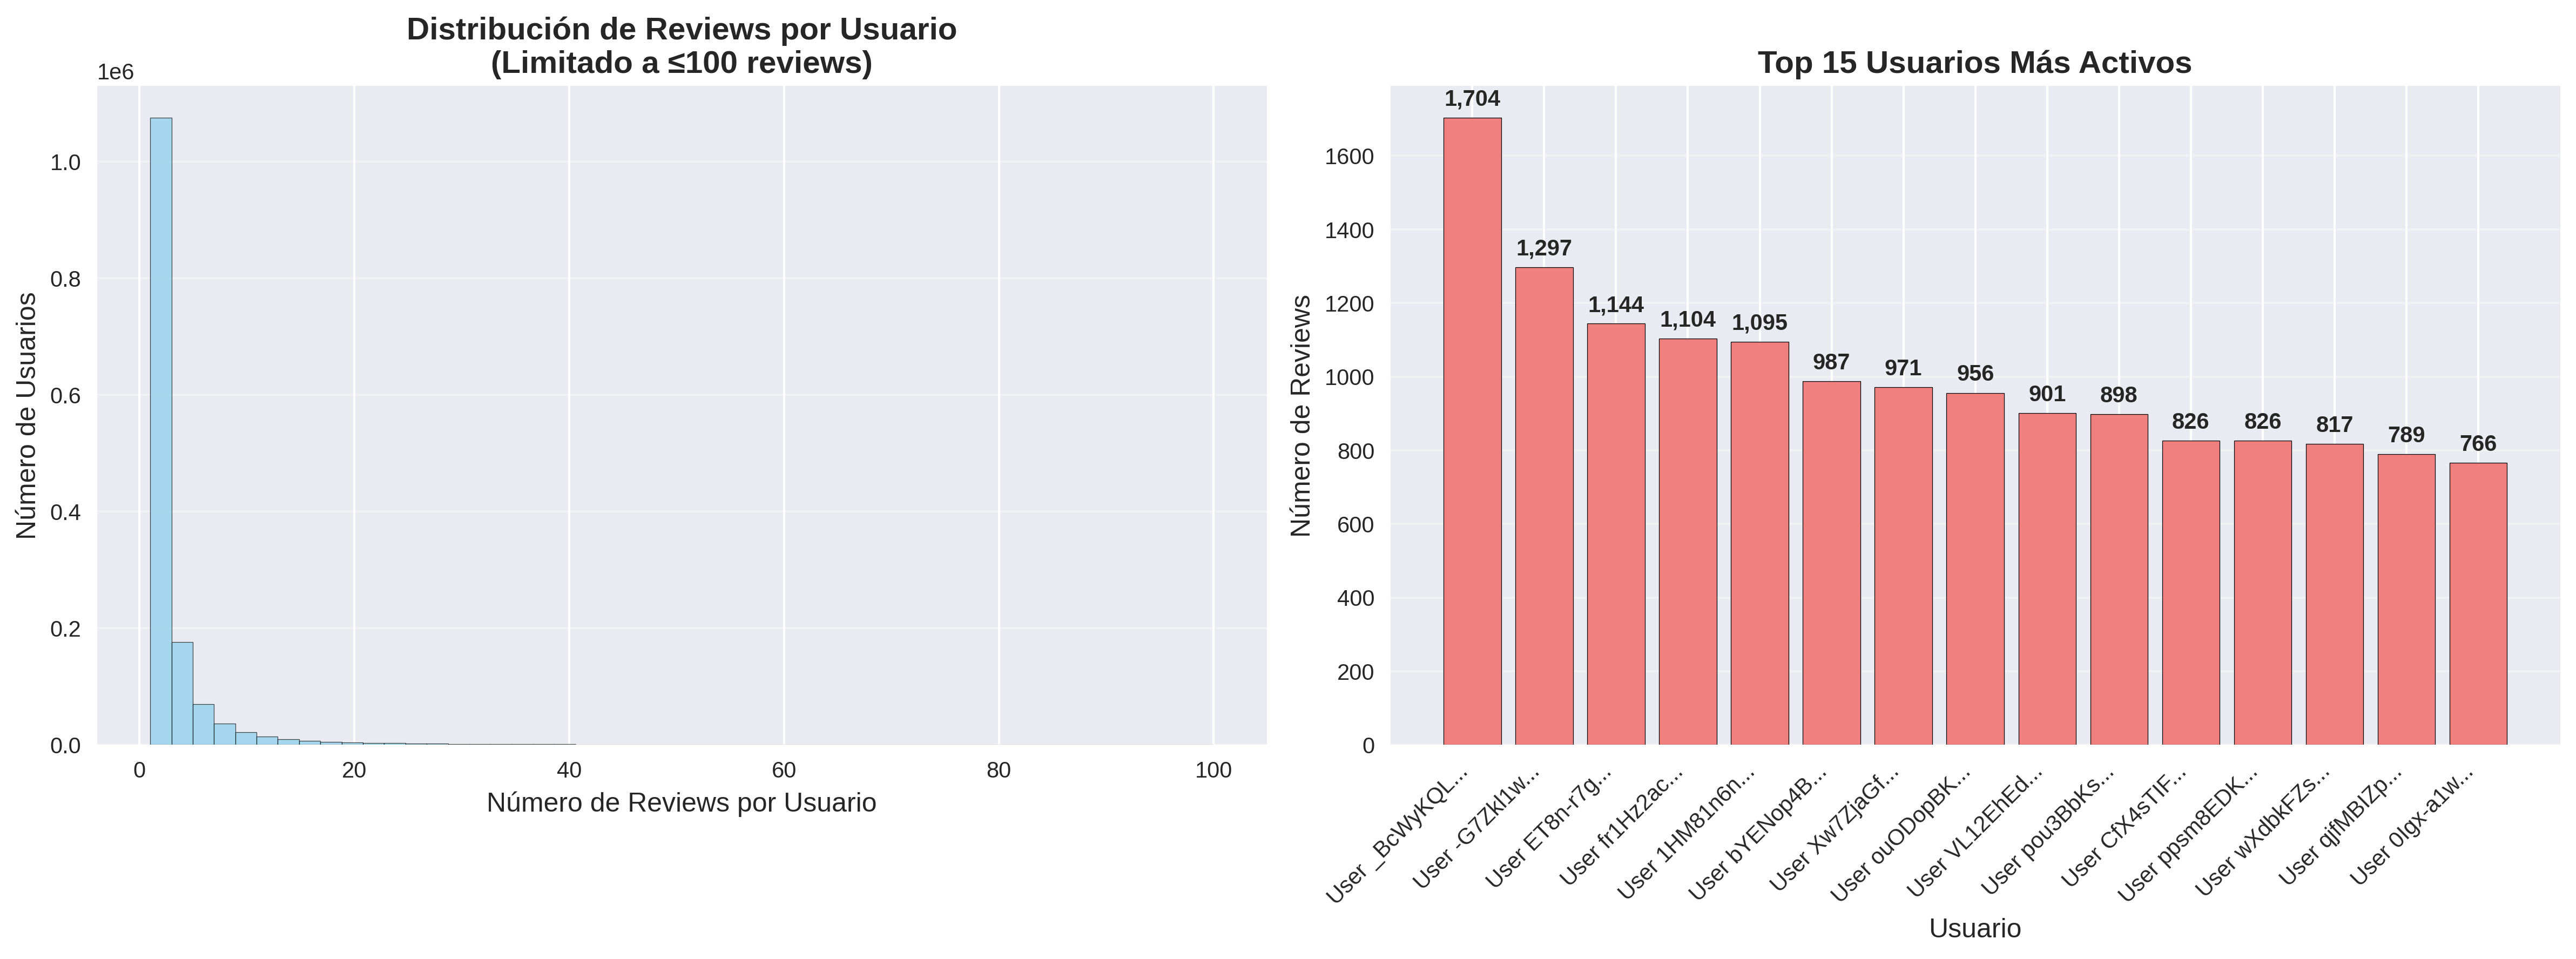
\includegraphics[width=0.9\textwidth]{figures/reviews_user_activity_analysis.png}
\caption{Análisis de actividad de usuarios por segmentos}
\label{fig:reviews_user_activity}
\end{figure}

La Figura~\ref{fig:reviews_user_activity} confirma la distribución de Pareto en la actividad de usuarios, donde la mayoría de usuarios contribuyen con pocas reseñas mientras que un pequeño porcentaje genera la mayor parte del contenido.

\subsection{Métricas de Engagement}

El análisis de engagement reveló patrones de interacción significativos:

Las estadísticas por métrica de engagement incluyen:

\begin{table}[H]
\centering
\caption{Métricas de engagement por categoría}
\begin{tabular}{@{}lrrr@{}}
\toprule
\textbf{Métrica} & \textbf{Promedio} & \textbf{Máximo} & \textbf{Participación} \\
\midrule
USEFUL & 0.984 & 420 & 41.7\% \\
FUNNY & 0.301 & 792 & 15.0\% \\
COOL & 0.480 & 404 & 22.8\% \\
\textbf{Total Combinado} & \textbf{1.765} & \textbf{1,011} & \textbf{47.6\%} \\
\bottomrule
\end{tabular}
\end{table}

\begin{figure}[H]
\centering
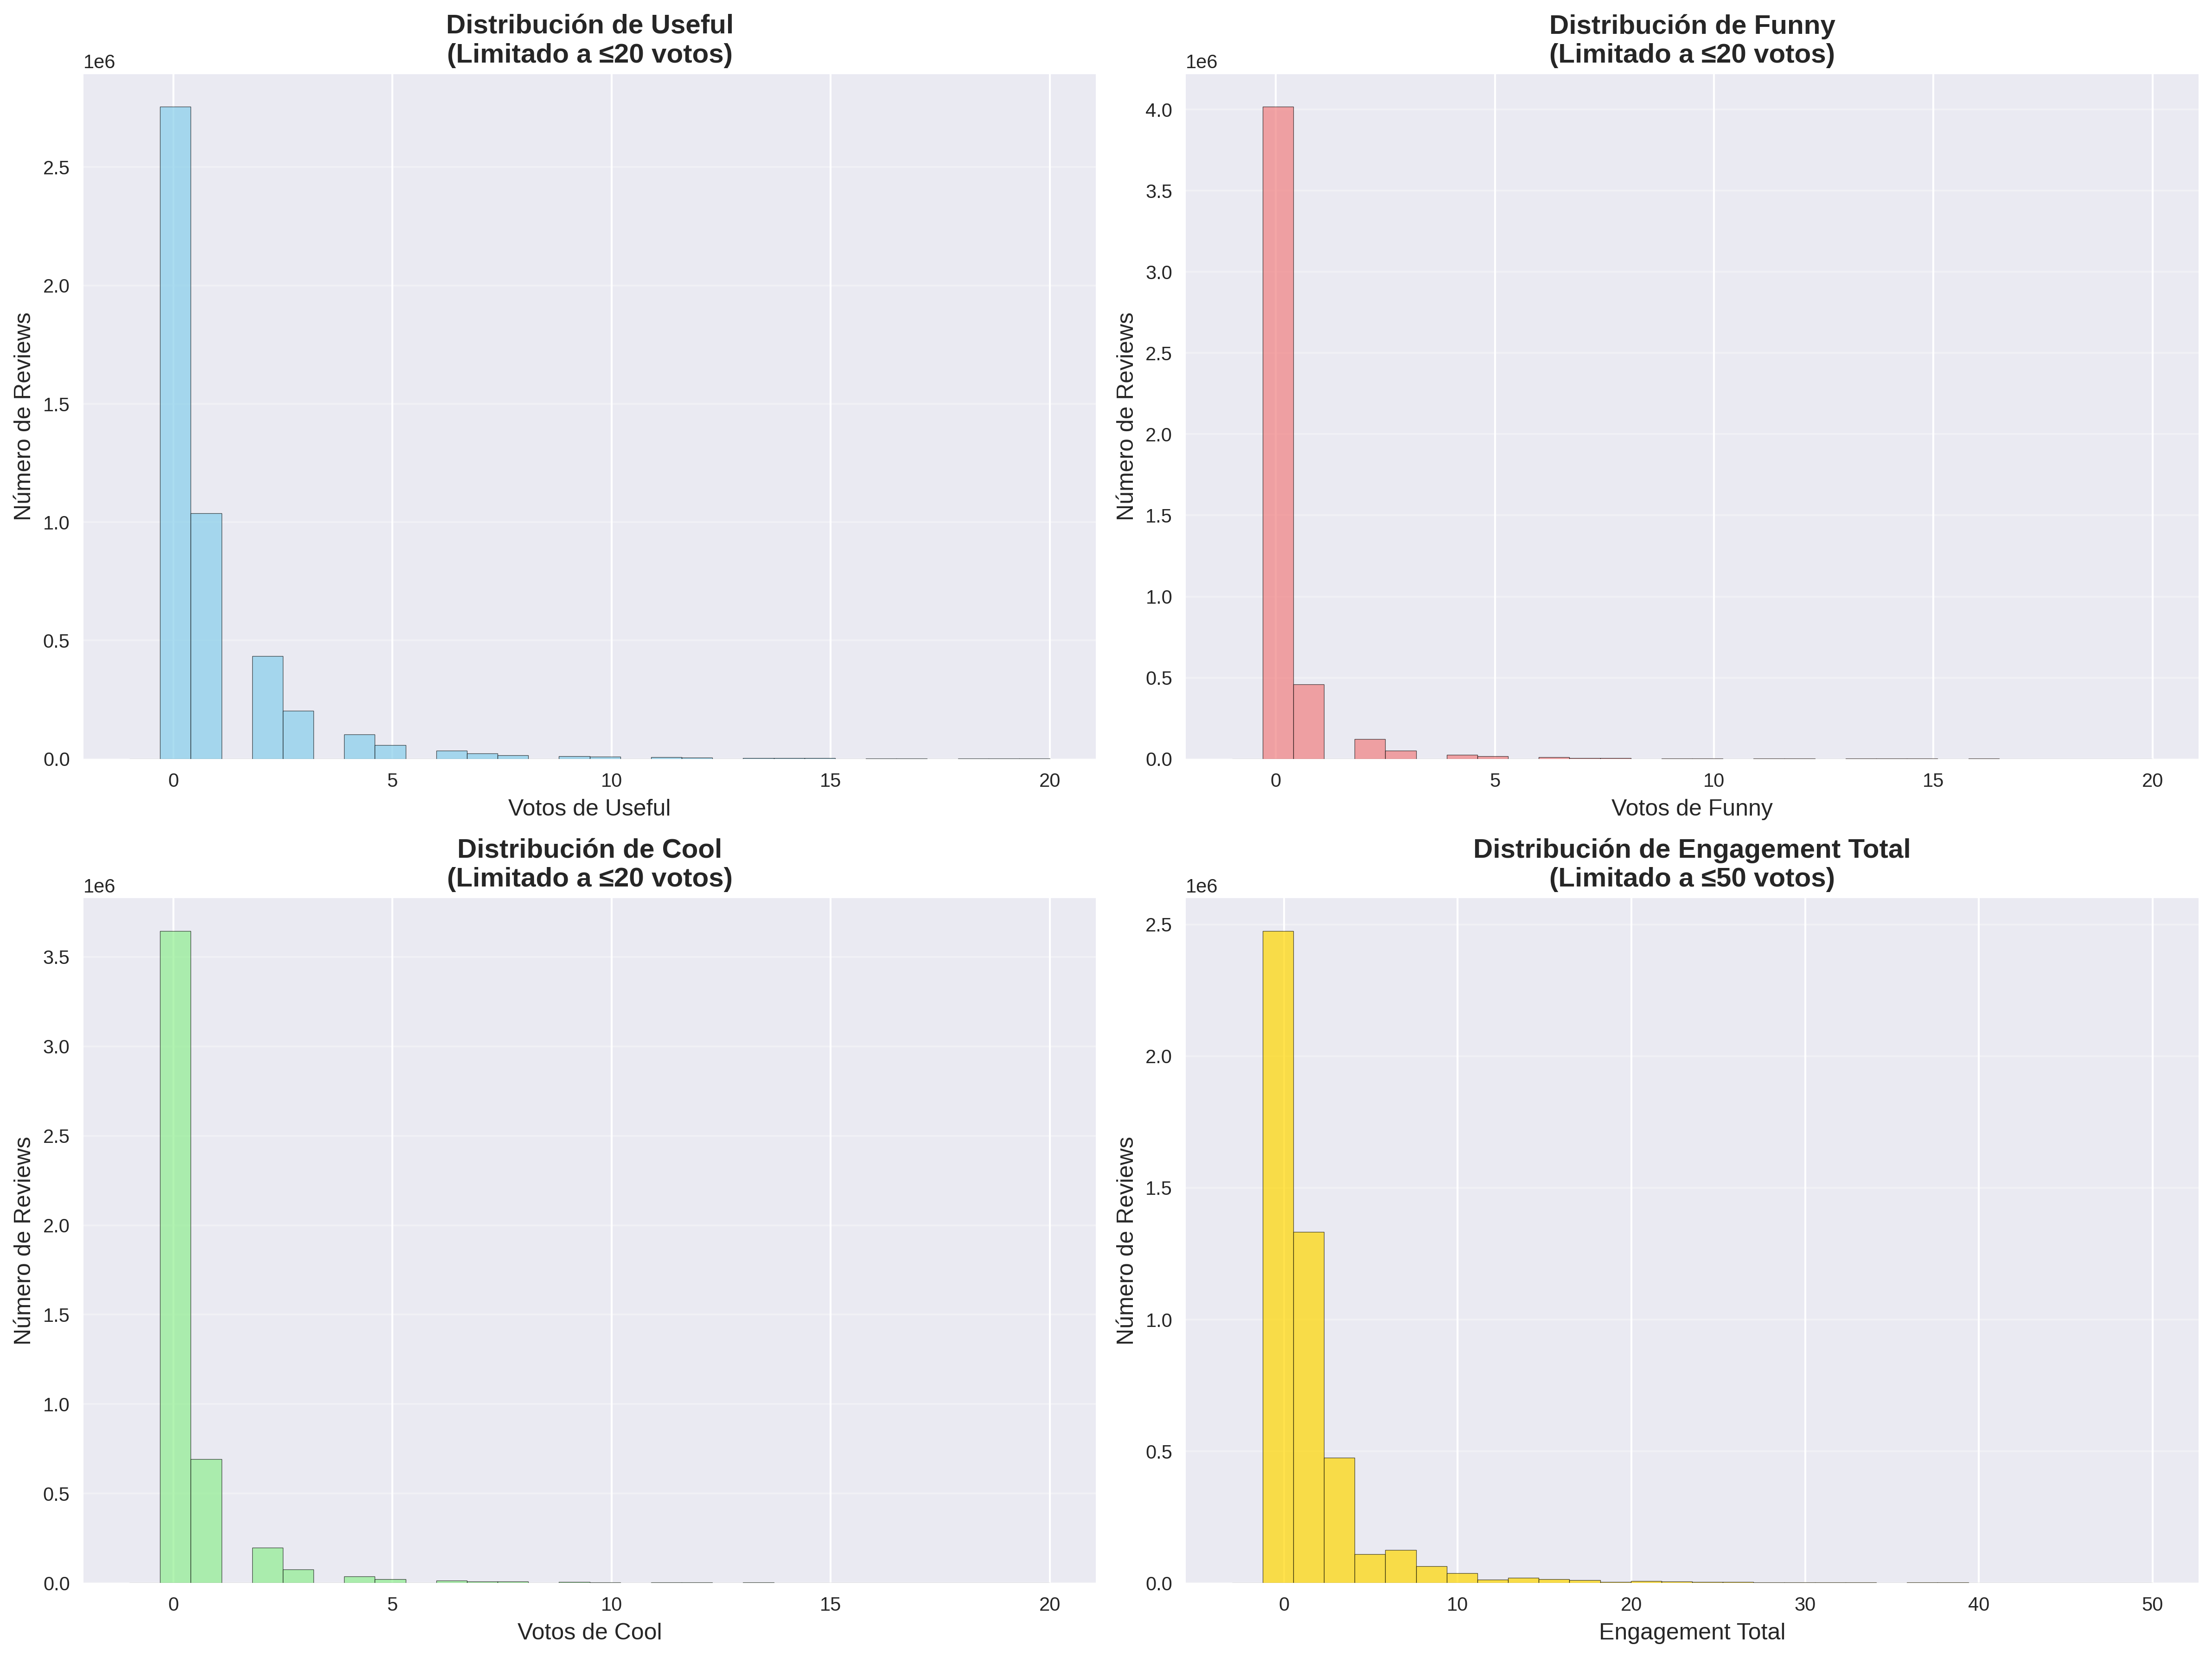
\includegraphics[width=0.9\textwidth]{figures/reviews_engagement_analysis.png}
\caption{Análisis de métricas de engagement en reseñas}
\label{fig:reviews_engagement}
\end{figure}

La Figura~\ref{fig:reviews_engagement} ilustra la distribución de las métricas de engagement, mostrando que ``useful'' es la métrica más utilizada por los usuarios para evaluar la utilidad de las reseñas, seguida por ``cool'' y ``funny''.

\section{Análisis Temporal}

\subsection{Evolución Temporal de Reseñas}

El análisis temporal revela la evolución del engagement y participación a lo largo de los 17 años de datos.

\begin{figure}[H]
\centering
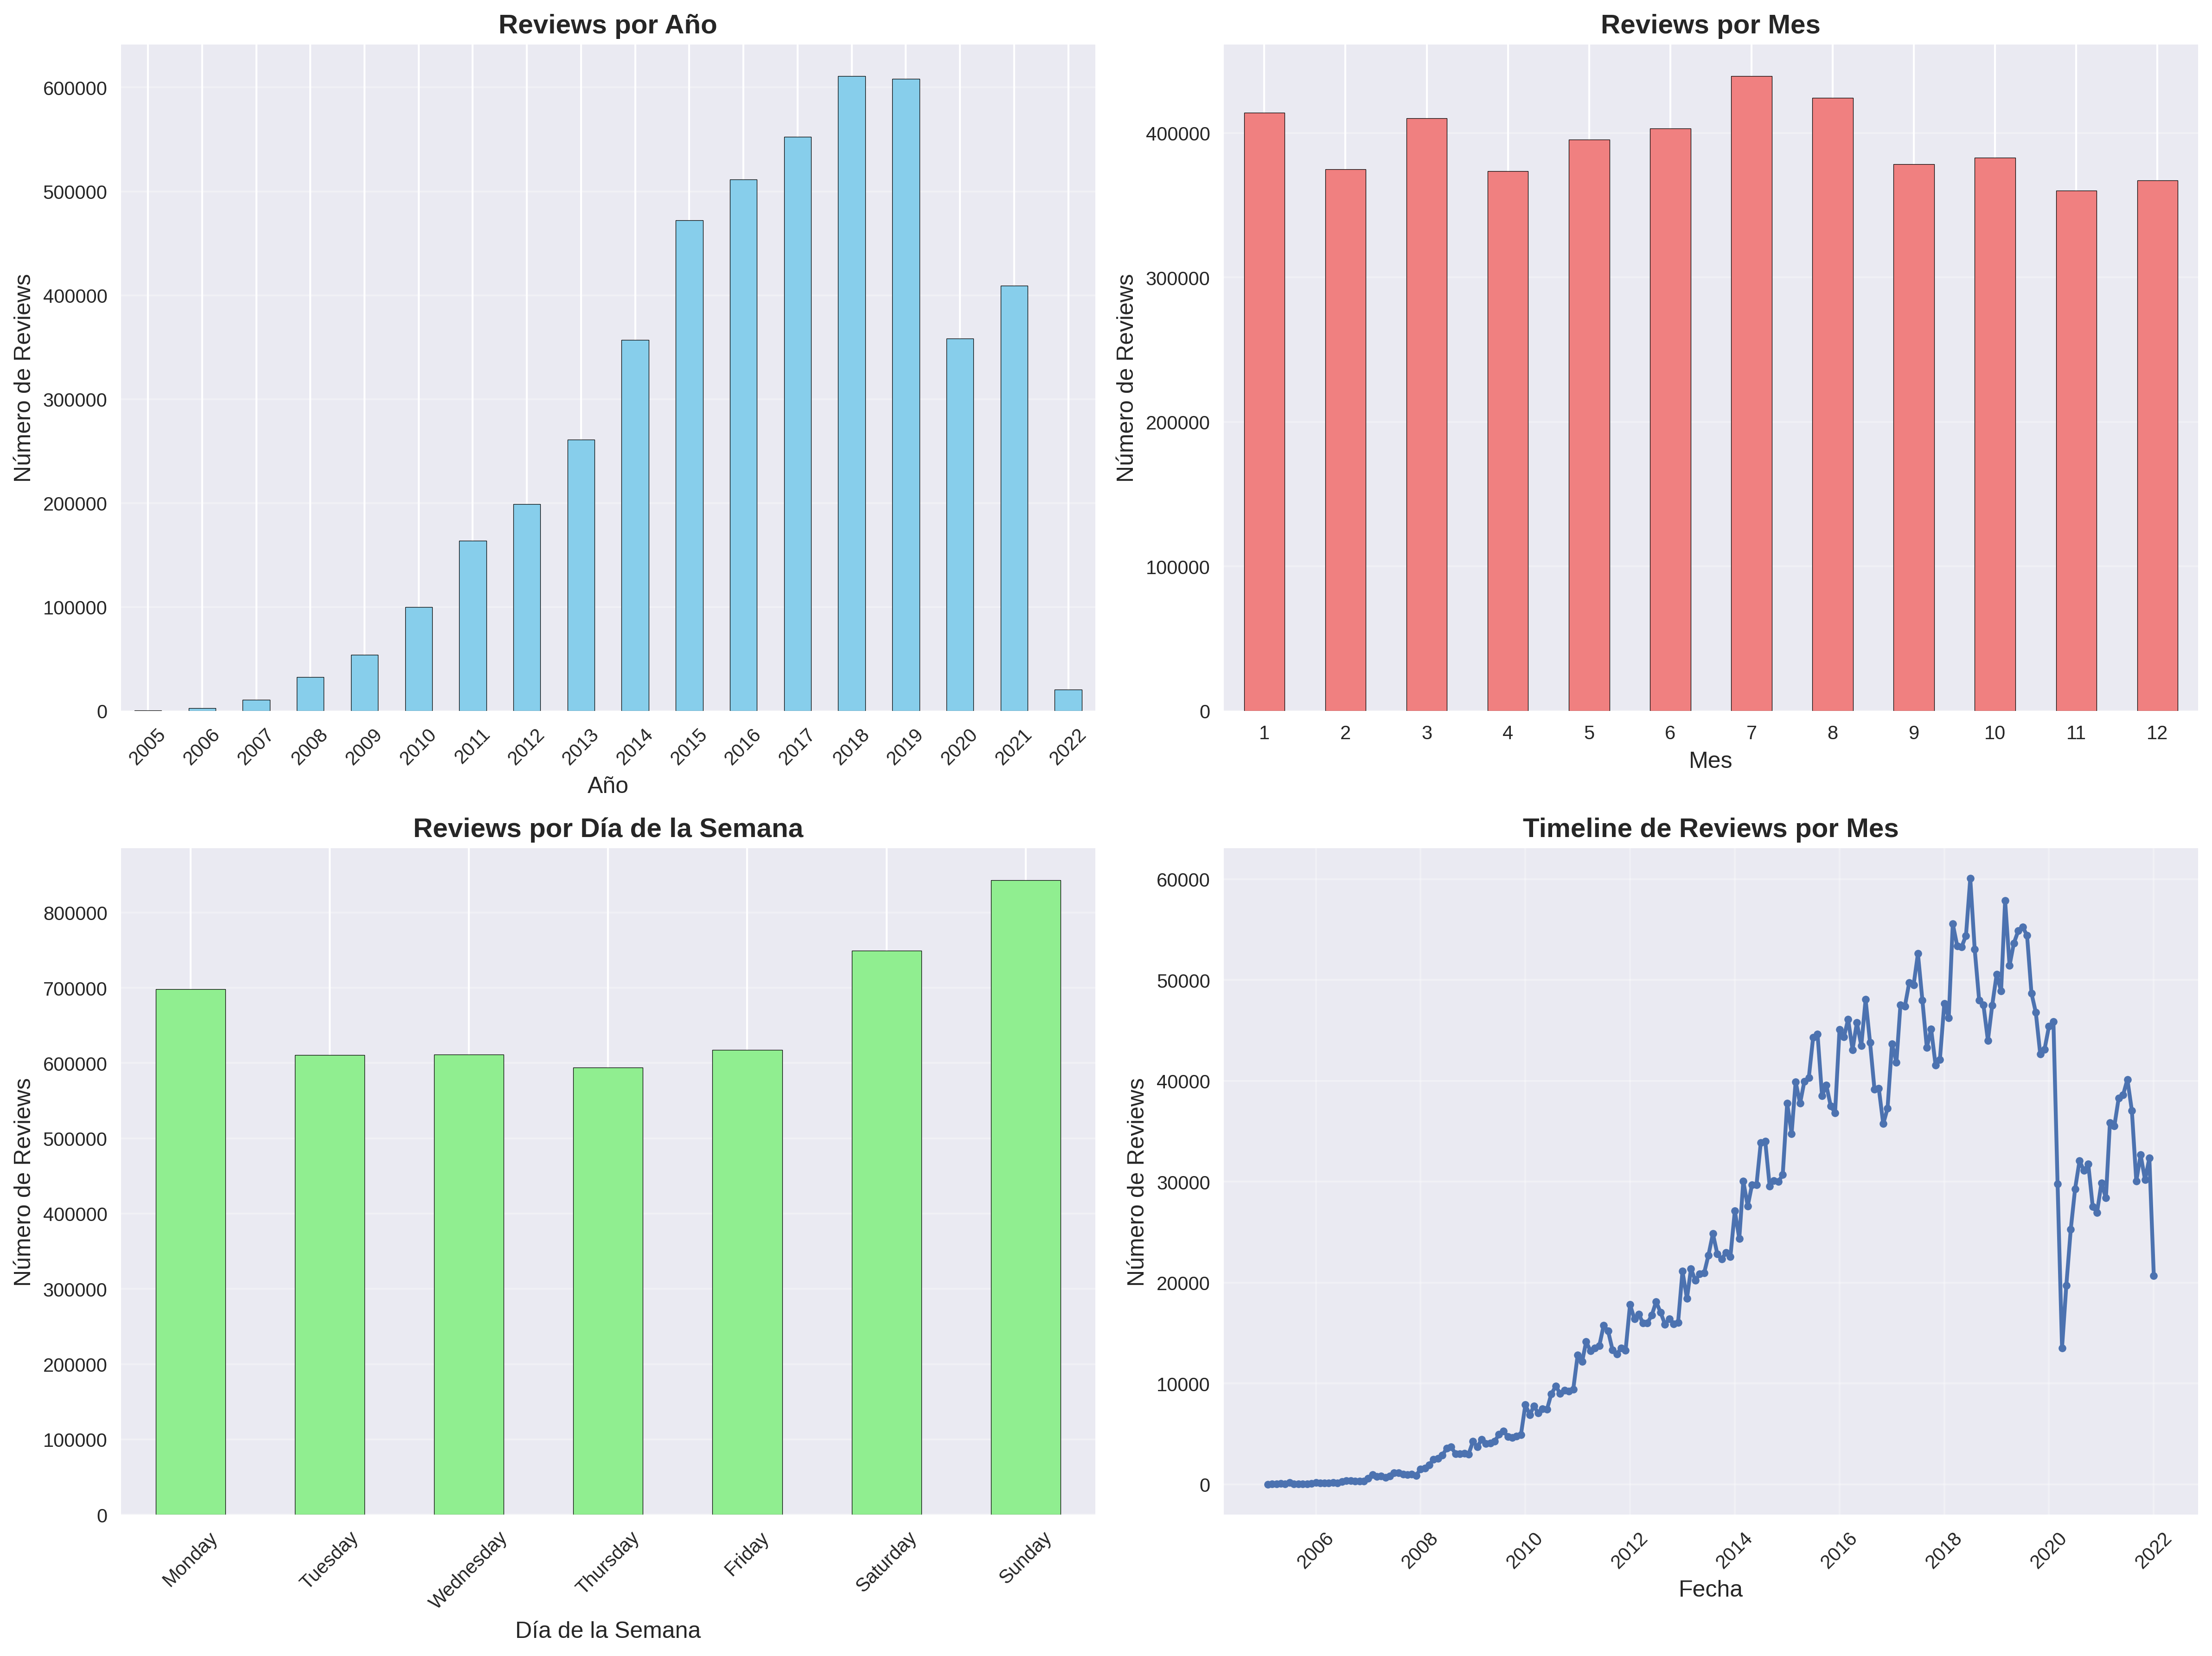
\includegraphics[width=1.0\textwidth]{figures/reviews_temporal_analysis.png}
\caption{Análisis temporal de reseñas (2005-2022)}
\label{fig:reviews_temporal_analysis}
\end{figure}

La Figura~\ref{fig:reviews_temporal_analysis} muestra la evolución temporal del volumen de reseñas, revelando un crecimiento exponencial del 2005 al 2016, seguido de una estabilización y posterior declive, posiblemente relacionado con la madurez de la plataforma y cambios en el comportamiento de usuarios.

\section{Análisis de Segmentación Avanzada}

\subsection{Metodología de Segmentación}

Se implementó un sistema de segmentación que permite análisis diferenciado por múltiples criterios:
\begin{itemize}
    \item Filtrado por calificaciones (mínimas/máximas)
    \item Filtrado por popularidad (número mínimo de reseñas)
    \item Segmentación geográfica
    \item Estado operacional
\end{itemize}

\subsection{Segmentos Identificados}

Los principales segmentos analizados incluyen:

\begin{table}[H]
\centering
\caption{Análisis comparativo de segmentos de mercado}
\begin{tabular}{@{}lrrrr@{}}
\toprule
\textbf{Segmento} & \textbf{Cantidad} & \textbf{Estrellas Prom.} & \textbf{Reviews Prom.} & \textbf{Estados} \\
\midrule
Dataset Completo & 52,268 & 3.52 & 90.39 & 19 \\
Alta Calidad & 7,460 & 4.18 & 317.77 & 14 \\
Premium & 1,189 & 4.51 & 513.87 & 14 \\
Mercado PA & 8,069 & 3.56 & 103.69 & 1 \\
\bottomrule
\end{tabular}
\end{table}

\begin{figure}[H]
\centering
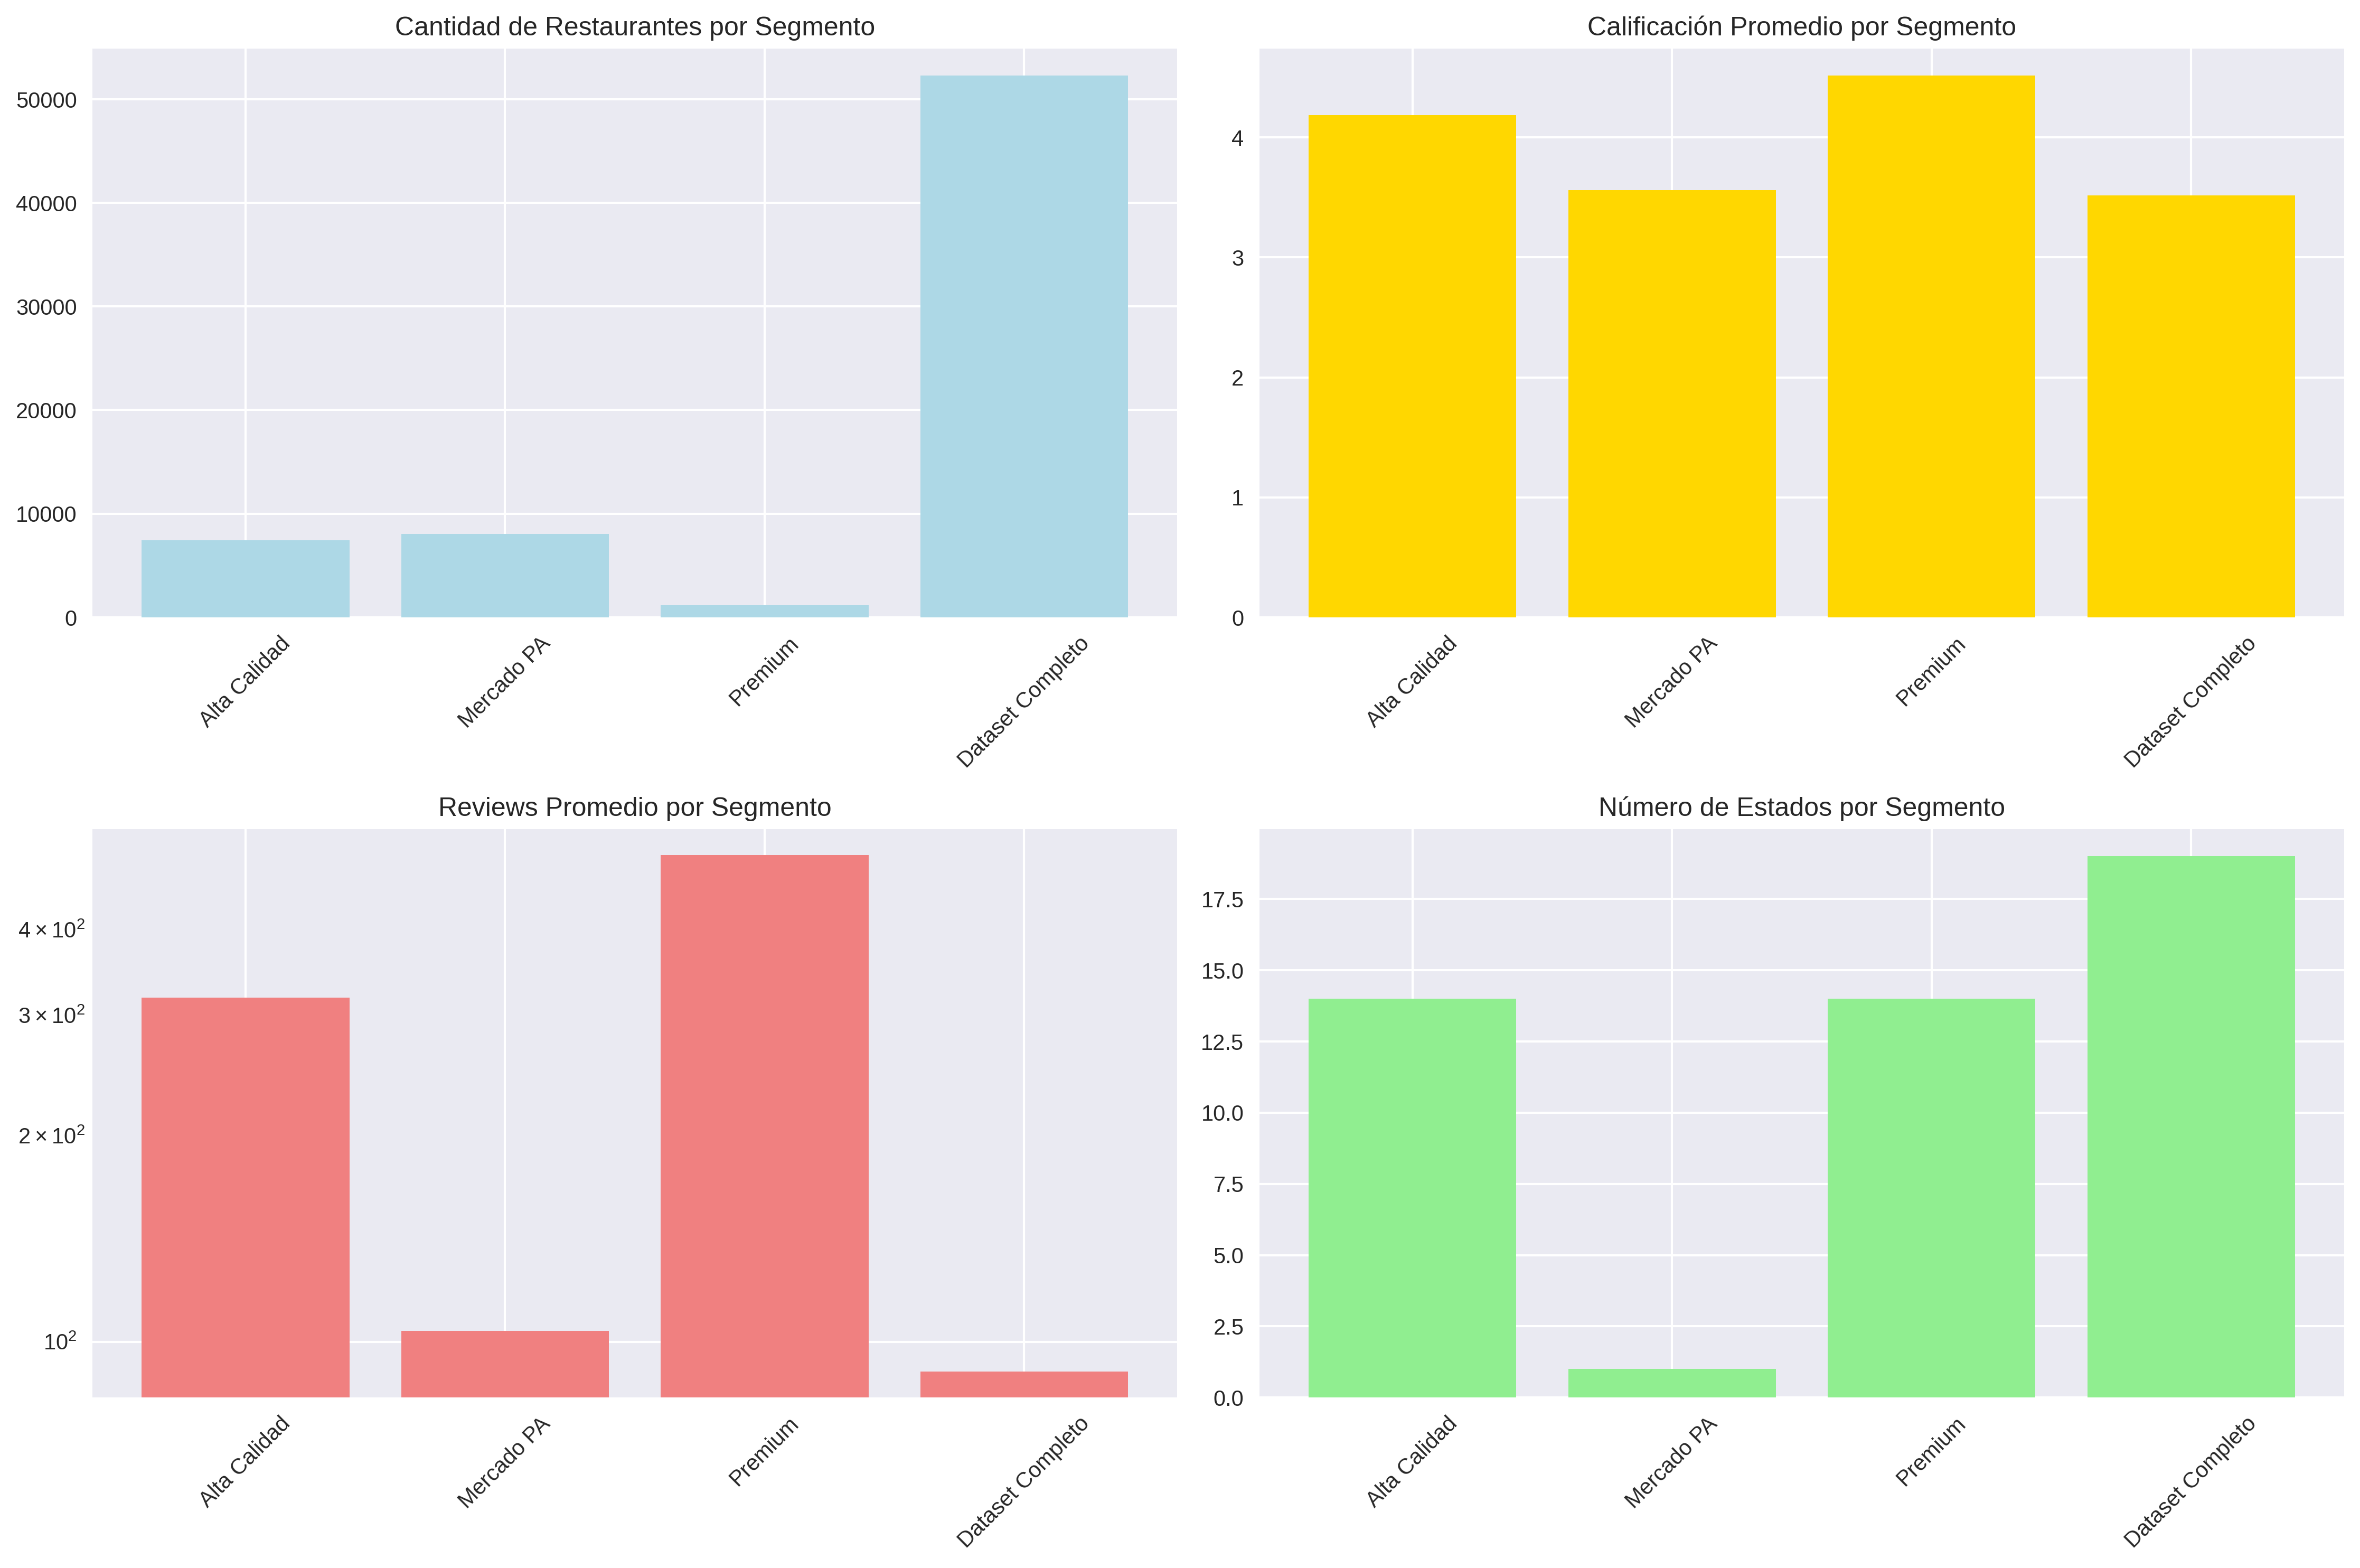
\includegraphics[width=0.8\textwidth]{figures/comparacion_segmentos.png}
\caption{Comparación de métricas clave entre segmentos de mercado}
\label{fig:comparacion_segmentos}
\end{figure}

La Figura~\ref{fig:comparacion_segmentos} visualiza las diferencias significativas entre segmentos, confirmando que los restaurantes de mayor calidad atraen más reseñas y mantienen calificaciones consistentemente altas.

\section{Correlaciones y Patrones}

\subsection{Correlación entre Métricas}

El análisis de correlaciones reveló relaciones significativas entre variables clave.

\begin{figure}[H]
\centering
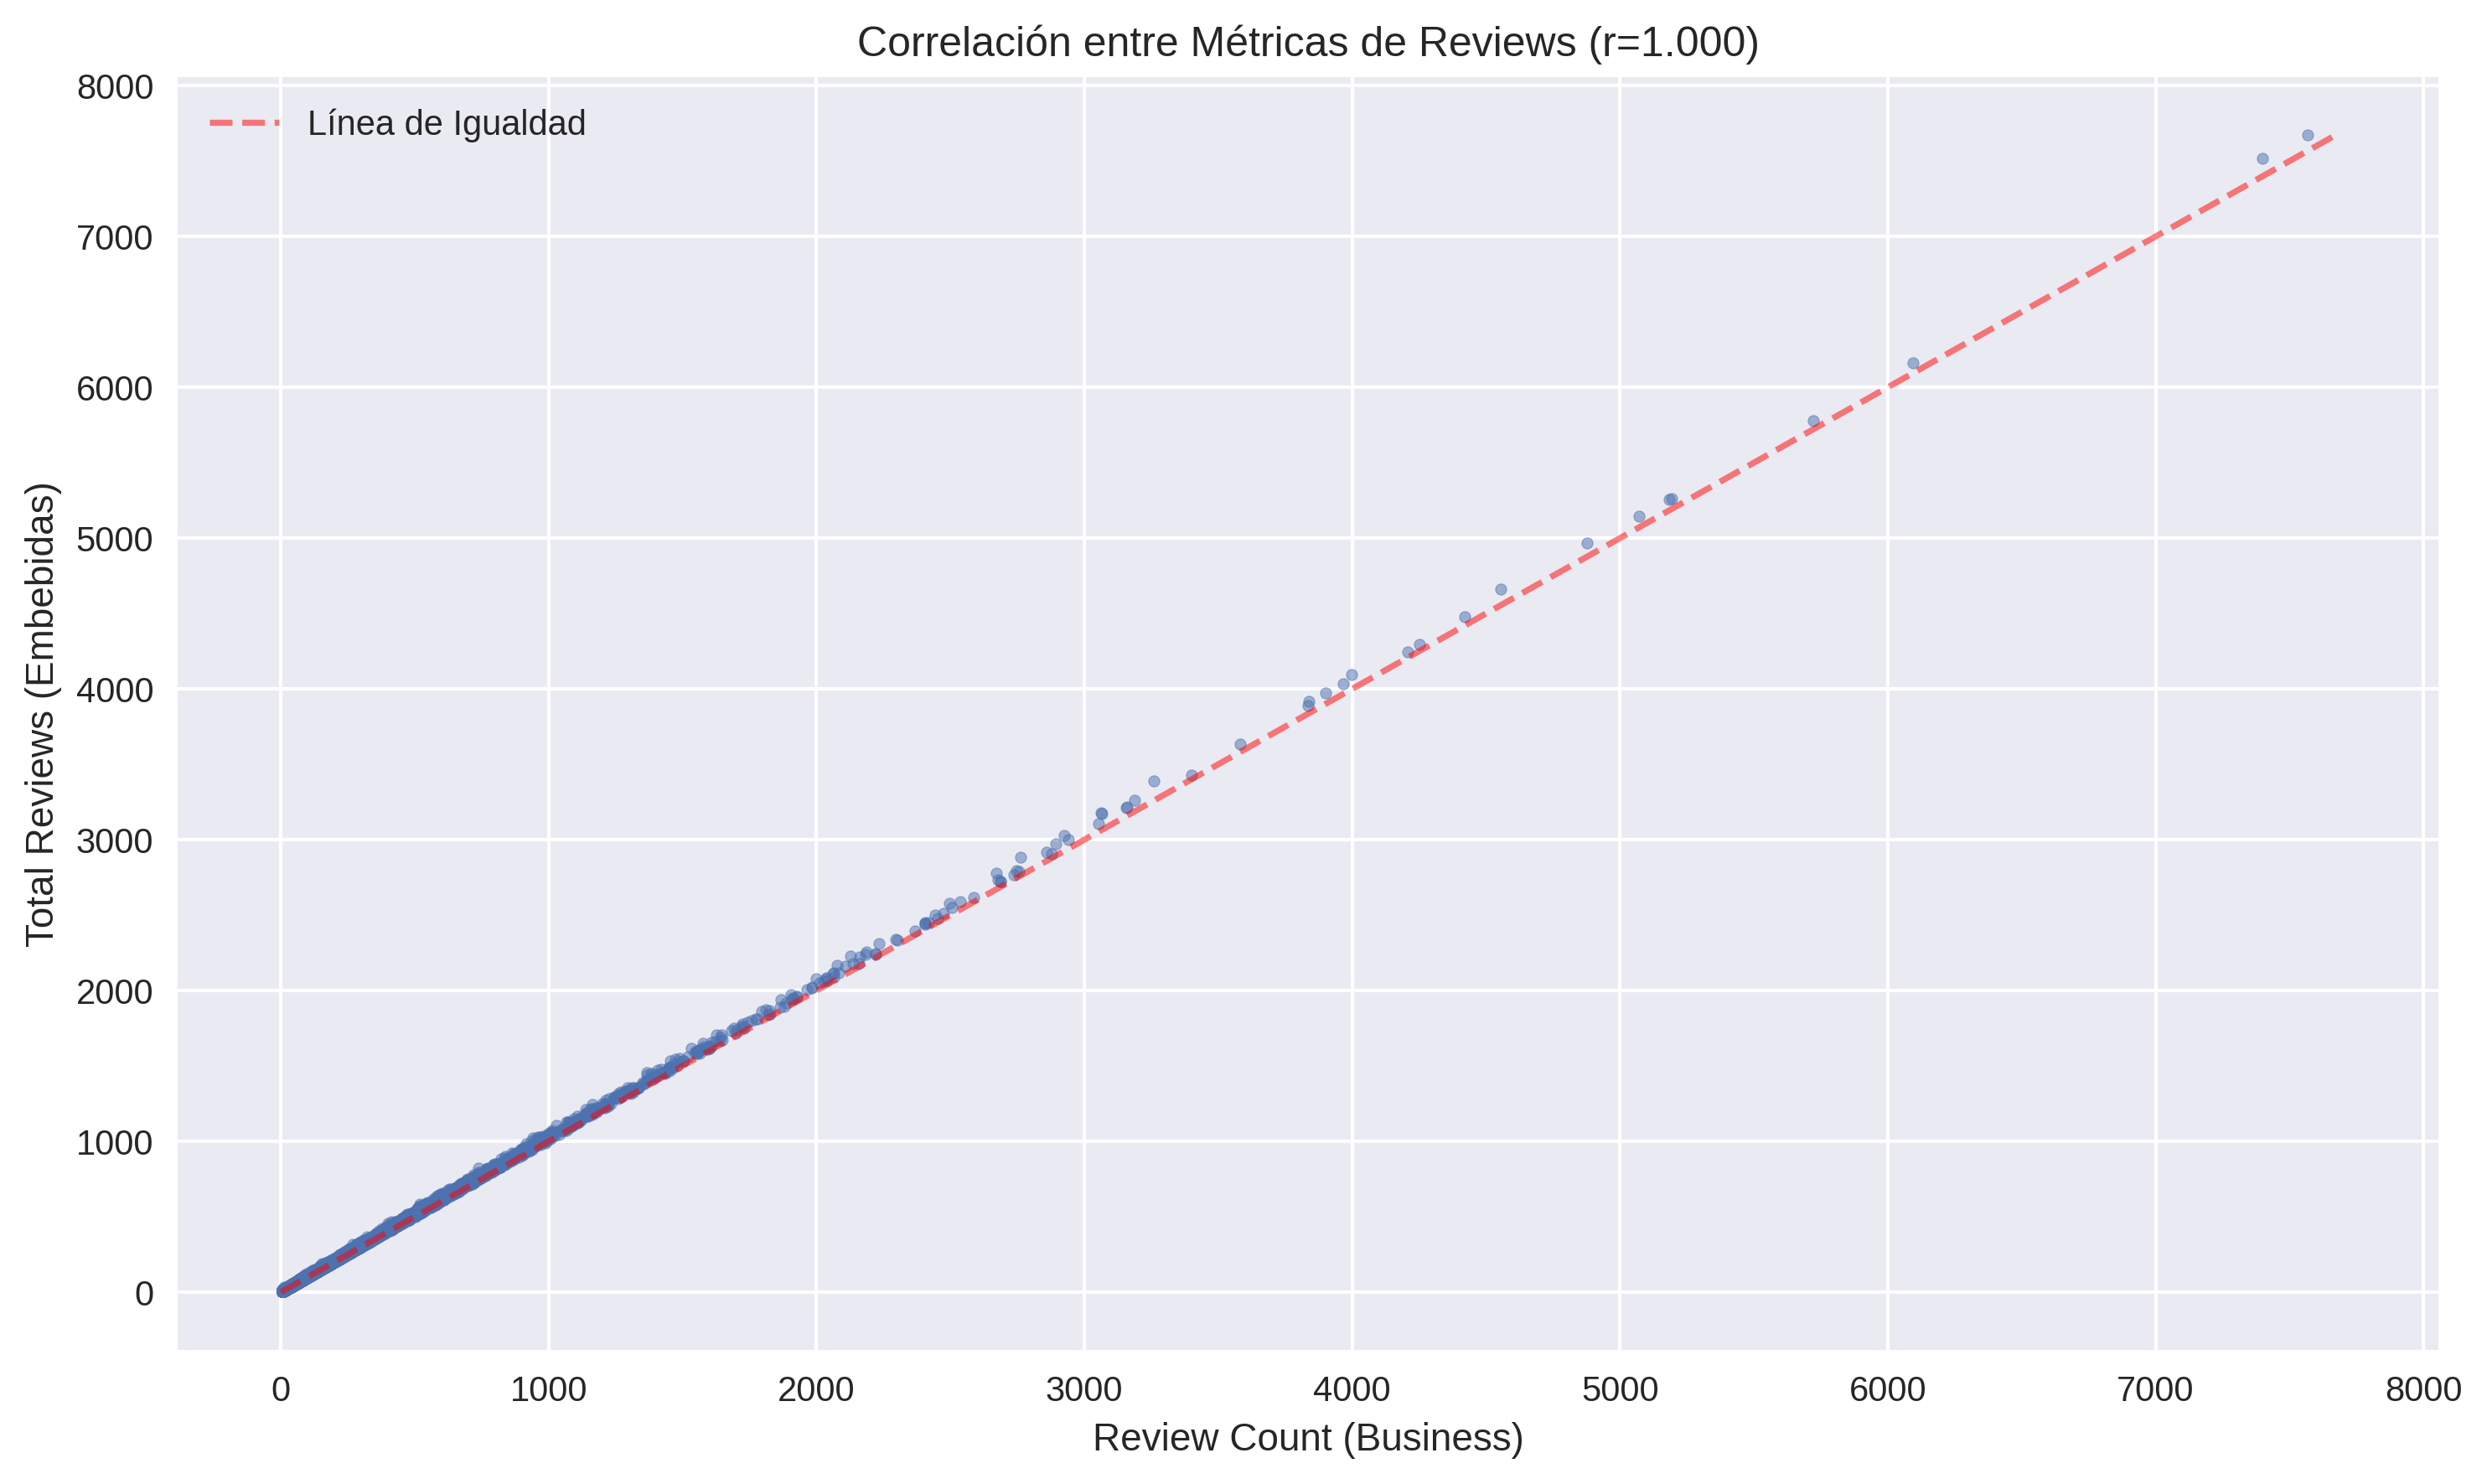
\includegraphics[width=0.8\textwidth]{figures/correlacion_metricas_reviews.png}
\caption{Matriz de correlación entre métricas de reseñas}
\label{fig:correlacion_metricas_reviews}
\end{figure}

\begin{figure}[H]
\centering
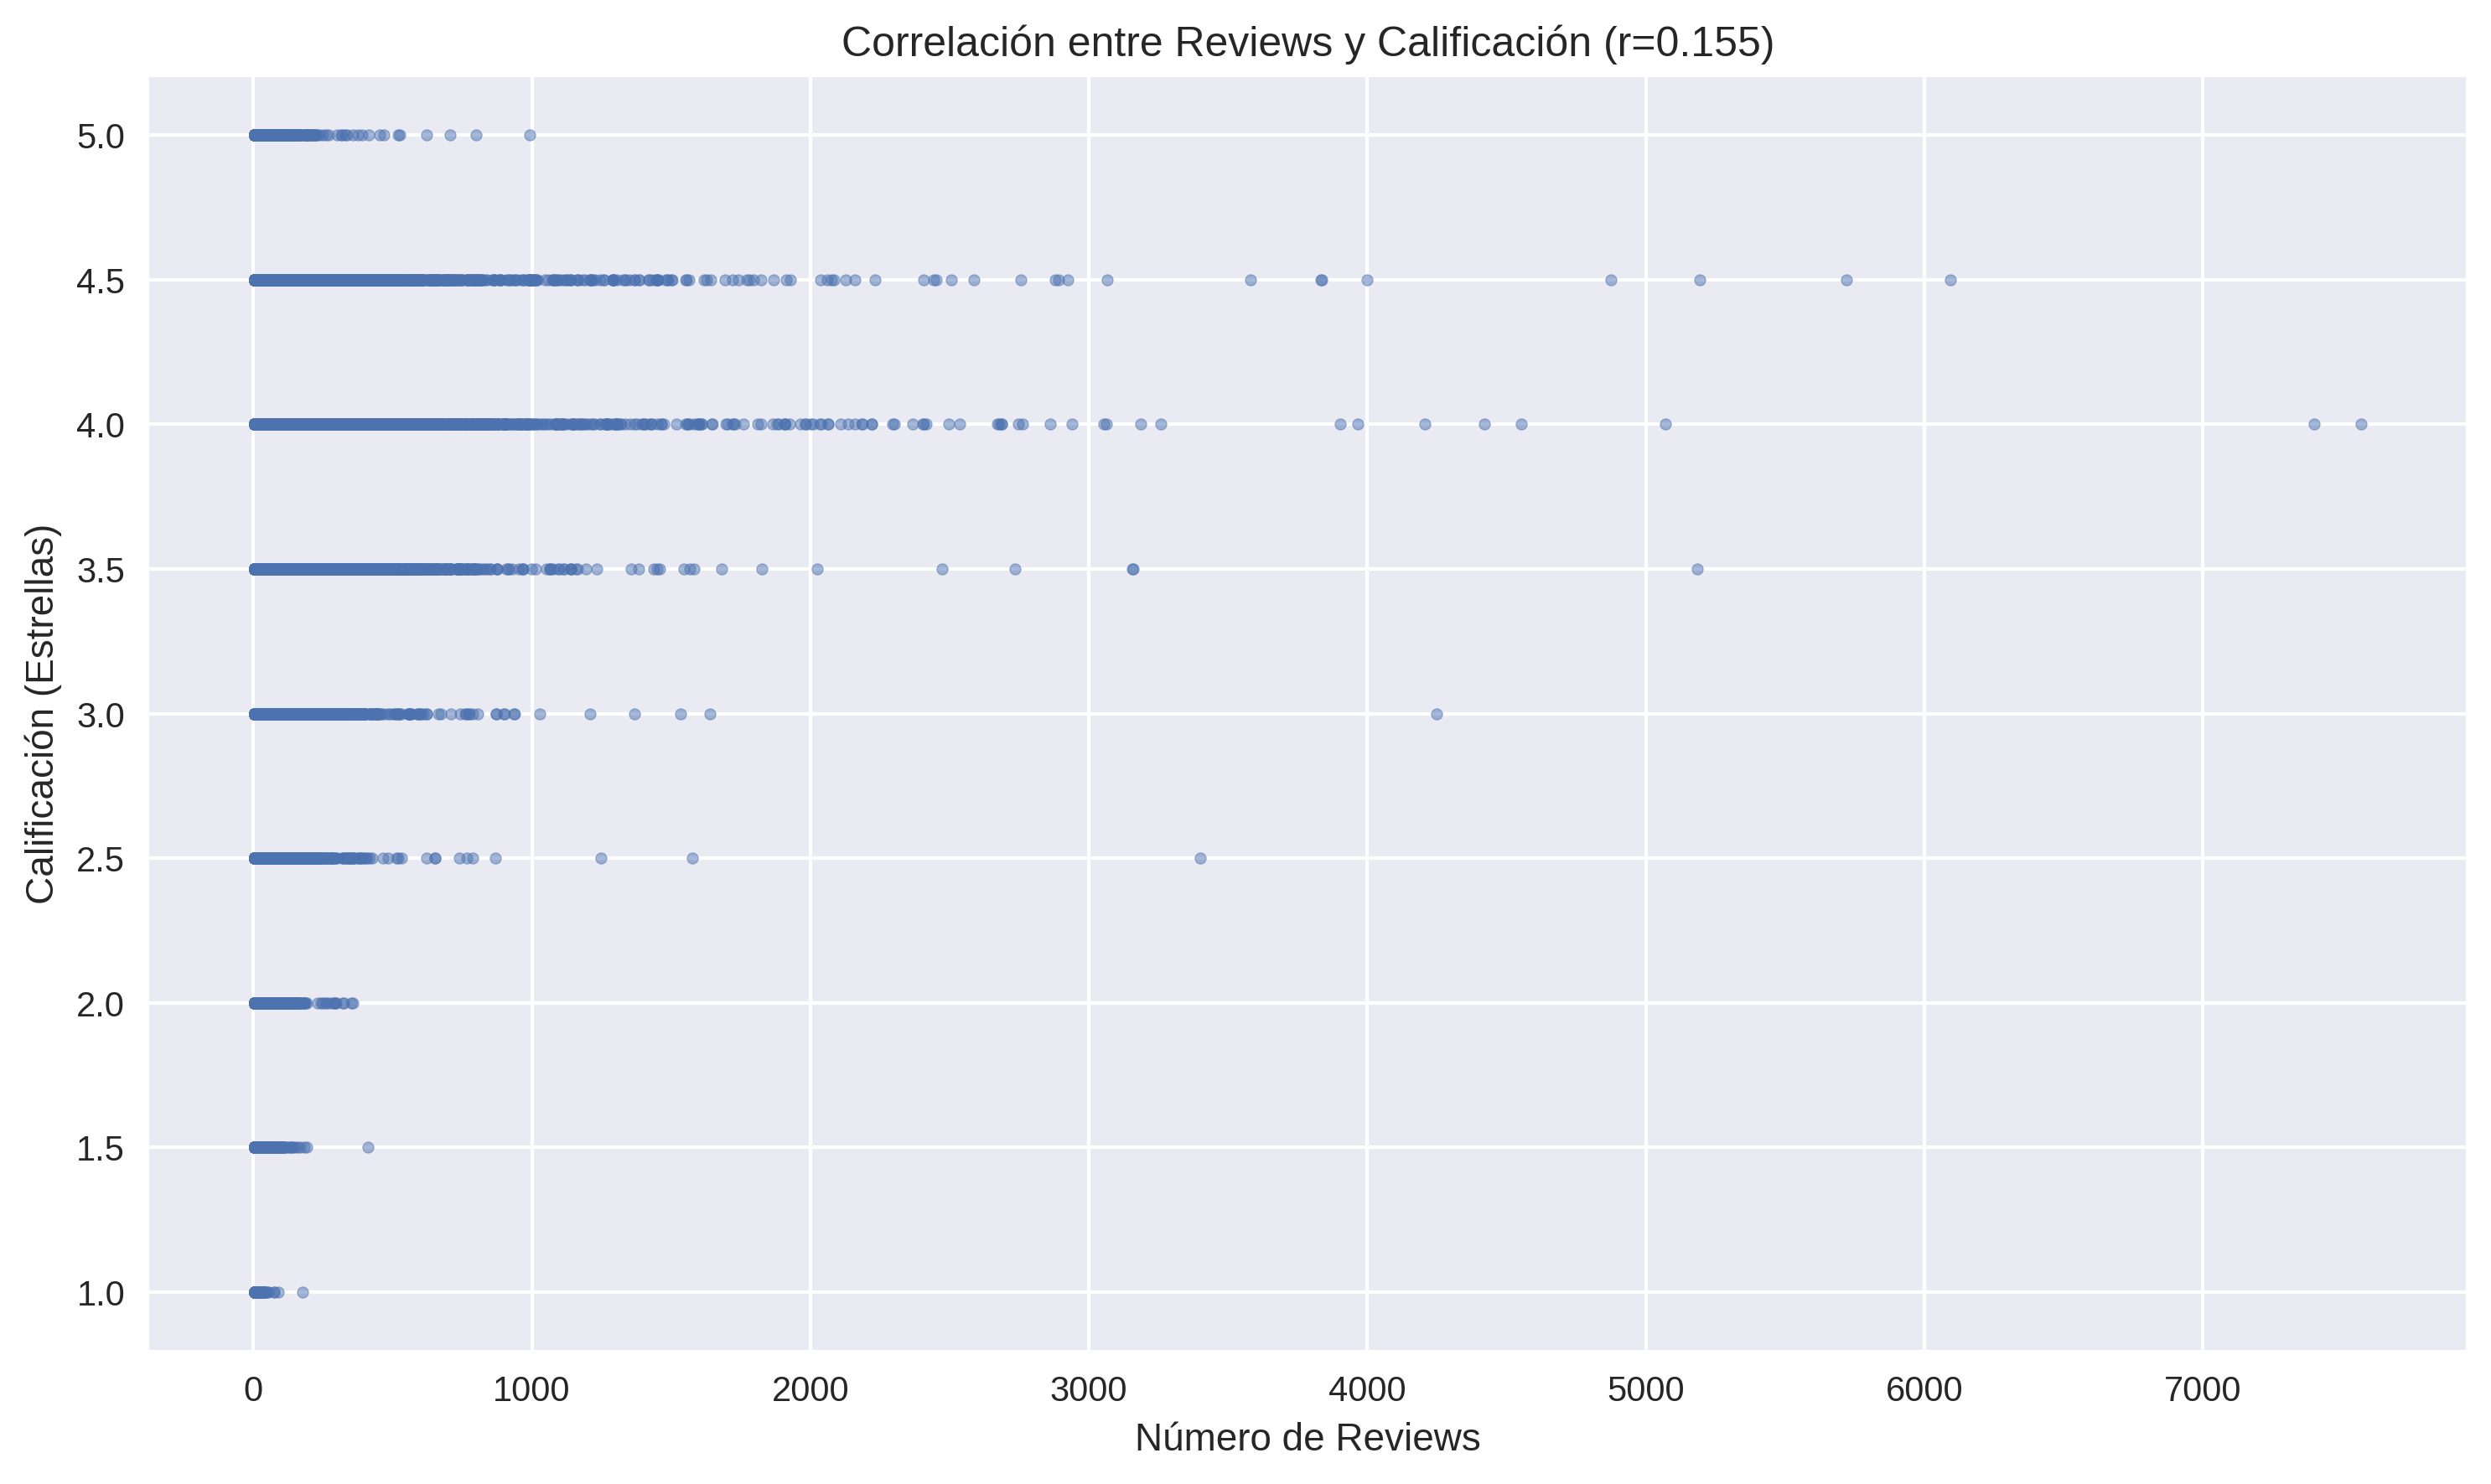
\includegraphics[width=0.8\textwidth]{figures/correlacion_reviews_calificacion.png}
\caption{Correlación entre número de reseñas y calificaciones}
\label{fig:correlacion_reviews_calificacion}
\end{figure}

Las Figuras~\ref{fig:correlacion_metricas_reviews} y~\ref{fig:correlacion_reviews_calificacion} muestran las relaciones entre diferentes métricas, revelando correlaciones positivas entre el número de reseñas y las calificaciones, así como patrones consistentes en las métricas de engagement.

\section{Insights y Conclusiones del Análisis Exploratorio}

\subsection{Hallazgos Principales}

El análisis exploratorio reveló patrones fundamentales:

\begin{enumerate}
    \item \textbf{Concentración geográfica}: Pennsylvania y Florida dominan el mercado con el 40.9\% de restaurantes
    \item \textbf{Sesgo positivo}: Las calificaciones muestran tendencia hacia valoraciones altas
    \item \textbf{Principio de Pareto en usuarios}: El 20\% de usuarios más activos genera el 67.1\% de reseñas
    \item \textbf{Correlación calidad-popularidad}: Los segmentos de mayor calidad atraen significativamente más reseñas
    \item \textbf{Diversidad gastronómica}: Amplia representación de categorías culinarias
\end{enumerate}

\subsection{Implicaciones para Análisis Posteriores}

Estos hallazgos establecen la base para:
\begin{itemize}
    \item \textbf{Análisis de sentimientos}: Validación de la correlación entre sentimientos y ratings
    \item \textbf{Modelado de tópicos}: Identificación de aspectos específicos que generan satisfacción/insatisfacción
    \item \textbf{Segmentación estratégica}: Análisis diferenciado por segmentos de calidad y geografía
    \item \textbf{Escalabilidad}: Confirmación de la viabilidad para procesamiento de grandes volúmenes
\end{itemize}

% Capítulo 6: Análisis de Sentimientos con RoBERTa
\chapter{Análisis de Sentimientos con \mbox{RoBERTa}}

\section{Introducción al Análisis de Sentimientos}

El análisis de sentimientos representa una de las aplicaciones más importantes del procesamiento de lenguaje natural en el contexto empresarial. Esta técnica permite automatizar la comprensión de actitudes, emociones y opiniones expresadas en texto no estructurado, proporcionando insights valiosos para la toma de decisiones empresariales.

En este proyecto, implementamos un sistema robusto utilizando el modelo RoBERTa preentrenado de Cardiff NLP, específicamente optimizado para el análisis de sentimientos en reseñas de restaurantes. La elección de RoBERTa se basó en su superior rendimiento en tareas de comprensión de lenguaje natural y su capacidad para capturar contextos complejos en texto corto.

\section{Fundamentos Teóricos}

\subsection{Arquitectura RoBERTa}

RoBERTa (Robustly Optimized BERT Pretraining Approach) es una versión optimizada de BERT que incorpora mejoras significativas en el proceso de preentrenamiento:

\begin{itemize}
    \item \textbf{Entrenamiento más largo}: Mayor número de épocas y datos de entrenamiento
    \item \textbf{Eliminación de NSP}: Remoción de la tarea de predicción de oración siguiente
    \item \textbf{Masking dinámico}: Patrones de masking variables durante el entrenamiento
    \item \textbf{Tamaño de batch mayor}: Optimización del proceso de entrenamiento
\end{itemize}

\subsection{Modelo Específico: Cardiff NLP}

El modelo seleccionado es ``twitter-roberta-base-sentiment'', que presenta las siguientes características:

\begin{itemize}
    \item \textbf{Dominio específico}: Preentrenado en datos de Twitter (texto corto)
    \item \textbf{Multiclase}: Clasificación en NEGATIVE, NEUTRAL, POSITIVE
    \item \textbf{Actualización reciente}: Modelo actualizado con datos recientes
    \item \textbf{Robustez}: Manejo efectivo de texto informal y abreviado
\end{itemize}

\section{Implementación Técnica}

\subsection{Configuración del Pipeline}

La implementación utiliza la biblioteca Transformers de Hugging Face para crear un pipeline optimizado, configurando el modelo twitter-roberta-base-sentiment con soporte para GPU cuando está disponible, truncamiento automático y mapeo de etiquetas.

\subsection{Preprocesamiento de Texto}

Se utilizó el pipeline de transformers con configuración básica, incluyendo truncamiento automático a 512 tokens y procesamiento directo del texto sin preprocesamiento específico adicional.

\subsection{Procesamiento por Lotes}

Para manejar eficientemente gran volumen de datos, se implementó procesamiento por lotes de 1000 textos, con seguimiento de progreso mediante tqdm y extracción de scores detallados para cada categoría de sentimiento.

\section{Optimización y Rendimiento}

\subsection{Métricas de Rendimiento}

Se implementaron métricas para monitorear el rendimiento del sistema, incluyendo medición de tiempo total, memoria utilizada, throughput y tiempo promedio por texto usando muestras de prueba.

\subsection{Resultados de Optimización}

Las optimizaciones implementadas resultaron en las siguientes mejoras:

\begin{table}[H]
\centering
\caption{Métricas de rendimiento del sistema de análisis de sentimientos}
\begin{tabular}{@{}lr@{}}
\toprule
\textbf{Métrica} & \textbf{Valor} \\
\midrule
Throughput promedio & 577 textos/segundo \\
Tiempo por texto & 0.002 segundos \\
Memoria utilizada & 16.9 GB GPU \\
Precisión del modelo & 82.6\% \\
Tiempo total (100K muestra) & 173 segundos \\
\bottomrule
\end{tabular}
\end{table}

\section{Análisis de Resultados}

\subsection{Distribución de Sentimientos}

El análisis de la muestra de 100,000 reseñas reveló la siguiente distribución:

\begin{table}[H]
\centering
\caption{Distribución de sentimientos en reseñas de restaurantes}
\begin{tabular}{@{}lrr@{}}
\toprule
\textbf{Sentimiento} & \textbf{Cantidad} & \textbf{Porcentaje} \\
\midrule
Positivo & 74,472 & 74.5\% \\
Negativo & 20,408 & 20.4\% \\
Neutral & 5,120 & 5.1\% \\
\textbf{Total} & \textbf{100,000} & \textbf{100.0\%} \\
\bottomrule
\end{tabular}
\end{table}

\subsection{Correlación con Ratings de Yelp}

Se analizó la correlación entre los resultados del análisis de sentimientos y los ratings numéricos de Yelp, convirtiendo sentimientos a valores numéricos y calculando correlaciones de Pearson y Spearman, junto con el análisis de distribución por rating.

\begin{table}[H]
\centering
\caption{Accuracy del modelo por rating de Yelp}
\begin{tabular}{@{}lrrr@{}}
\toprule
\textbf{Rating Yelp} & \textbf{Reviews} & \textbf{Accuracy} & \textbf{Confianza} \\
\midrule
1 estrella & 12,026 & 85.1\% & 0.814 \\
2 estrellas & 8,558 & 68.0\% & 0.740 \\
3 estrellas & 11,292 & 12.6\% & 0.740 \\
4 estrellas & 23,727 & 92.0\% & 0.884 \\
5 estrellas & 44,397 & 97.6\% & 0.946 \\
\bottomrule
\end{tabular}
\end{table}

El análisis muestra una correlación fuerte entre las predicciones del modelo y los ratings originales, con excelente rendimiento en ratings extremos (1 y 5 estrellas) y menor precisión en ratings neutros (3 estrellas).

\begin{figure}[H]
\centering
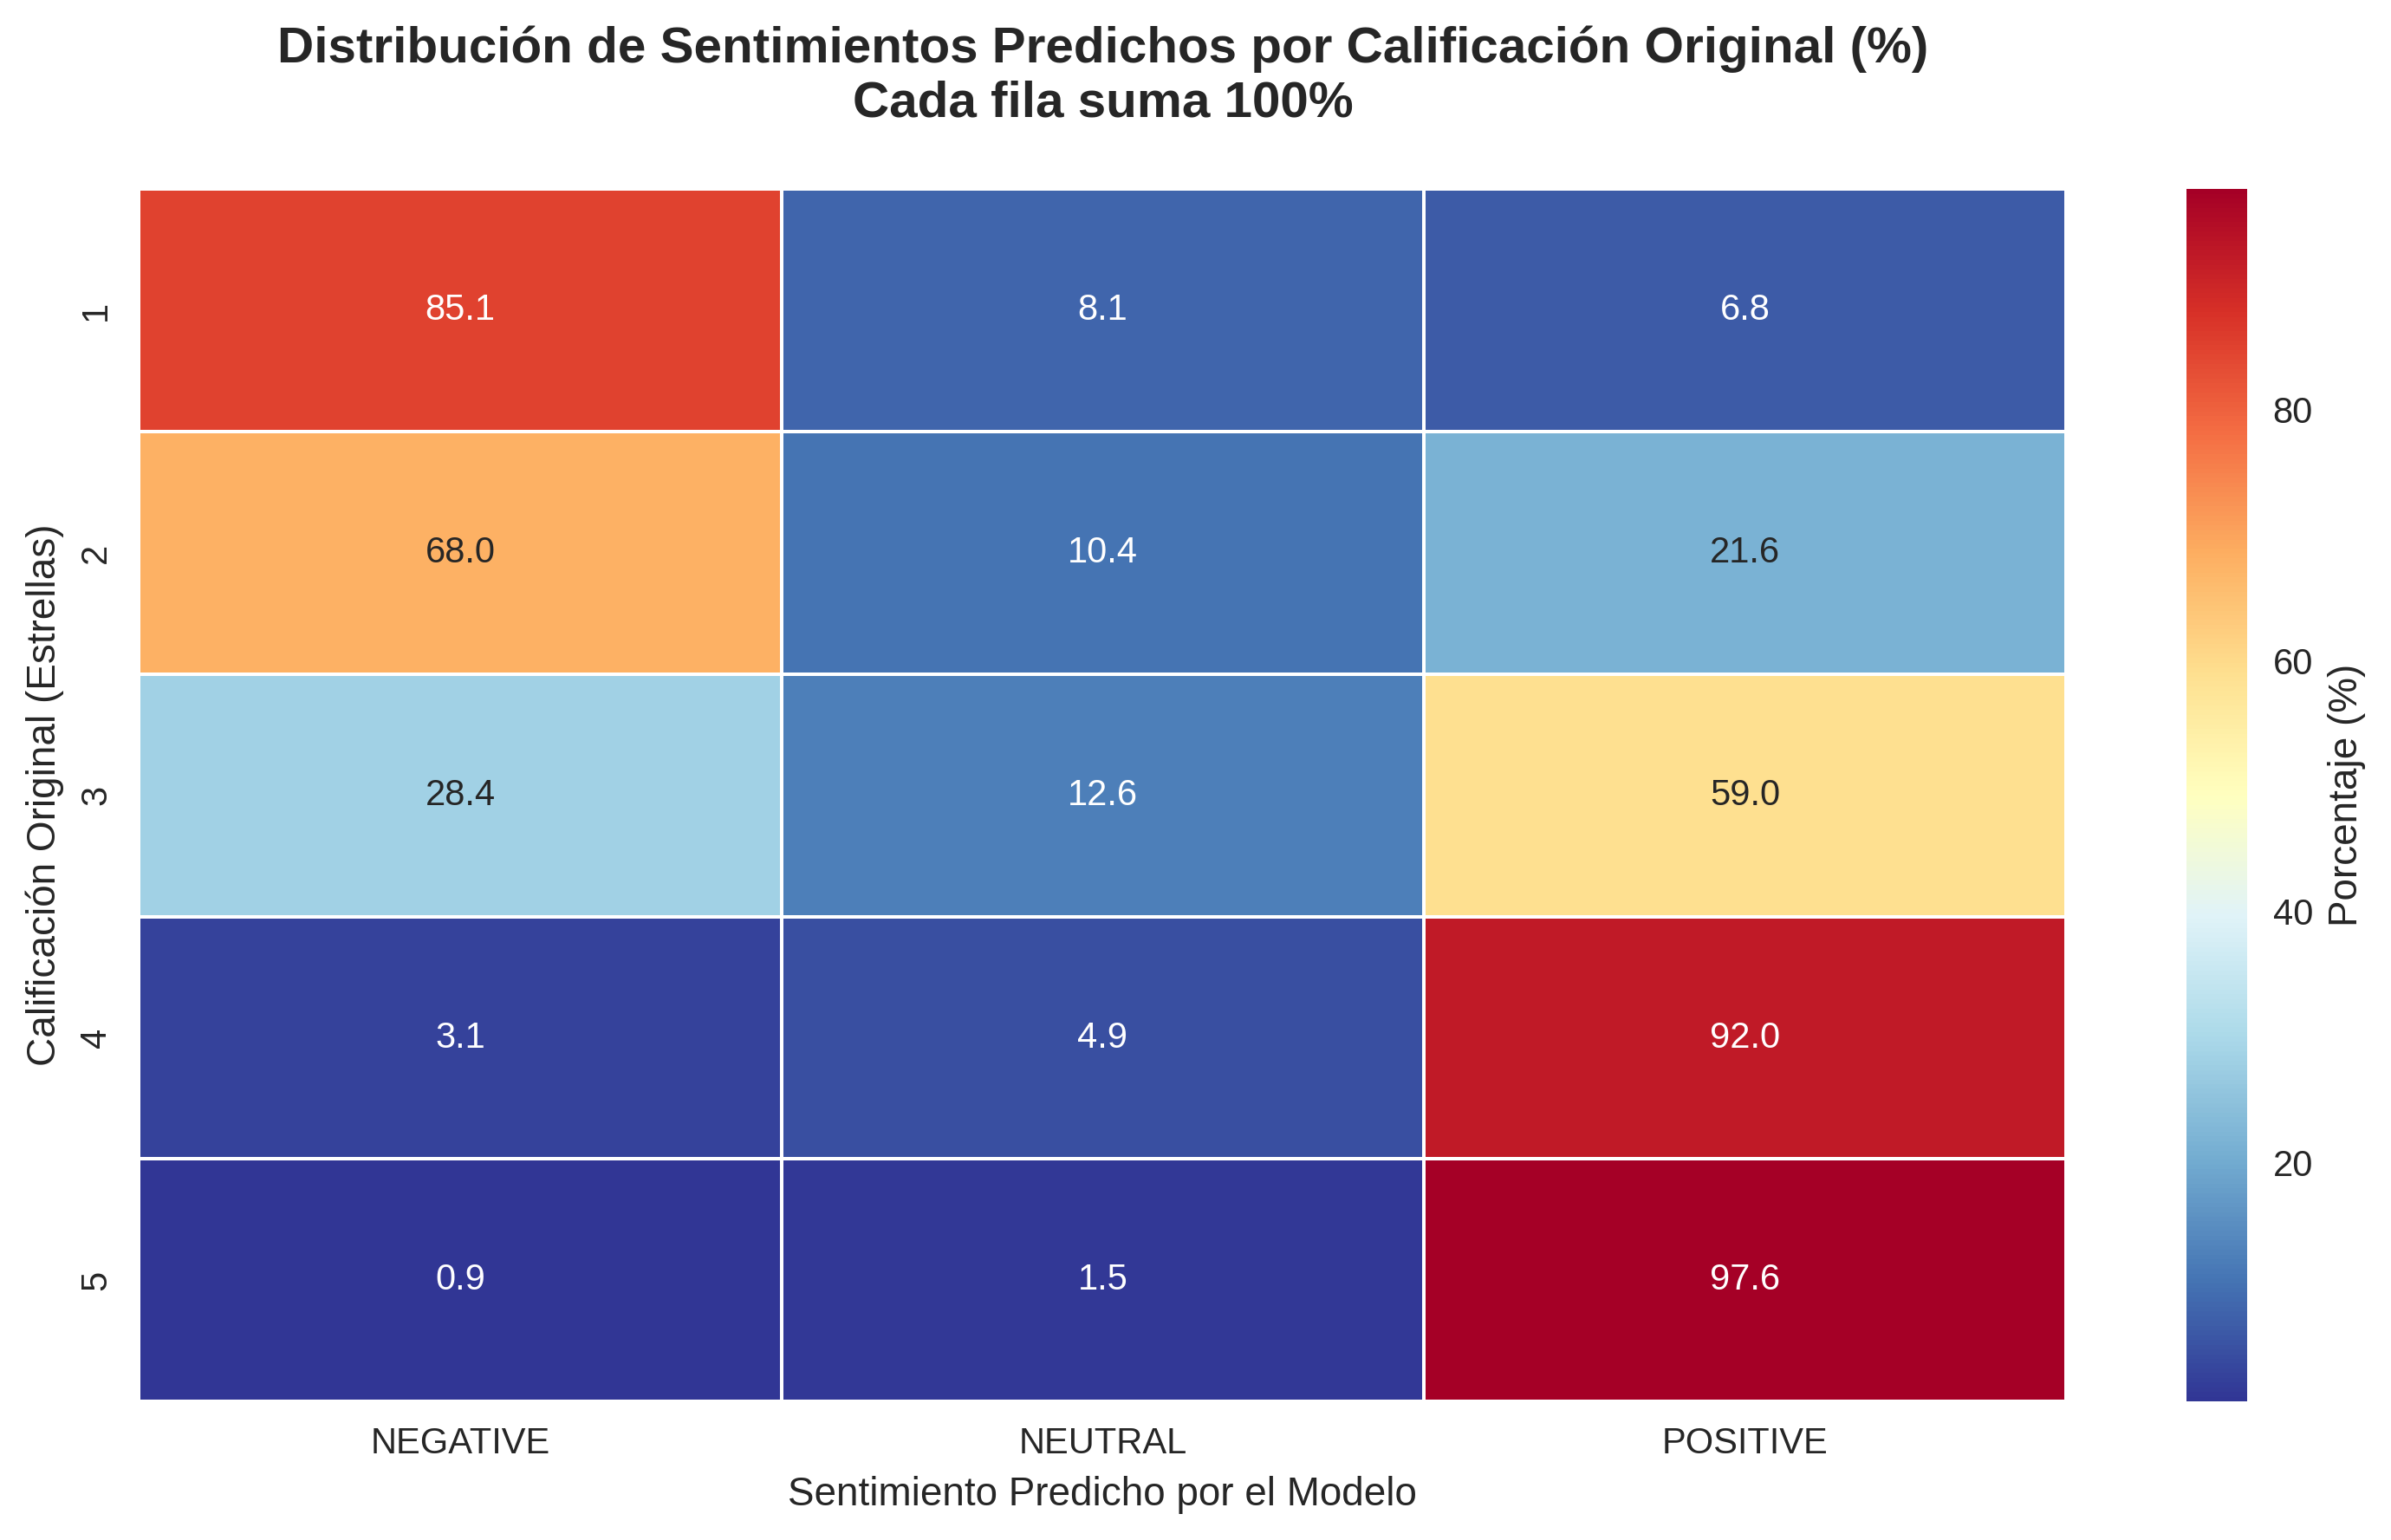
\includegraphics[width=0.8\textwidth]{figures/sentiment_prediction_correlation_heatmap.png}
\caption{Mapa de calor de correlación entre predicciones de sentimiento y ratings}
\label{fig:sentiment_correlation_heatmap}
\end{figure}

\begin{figure}[H]
\centering
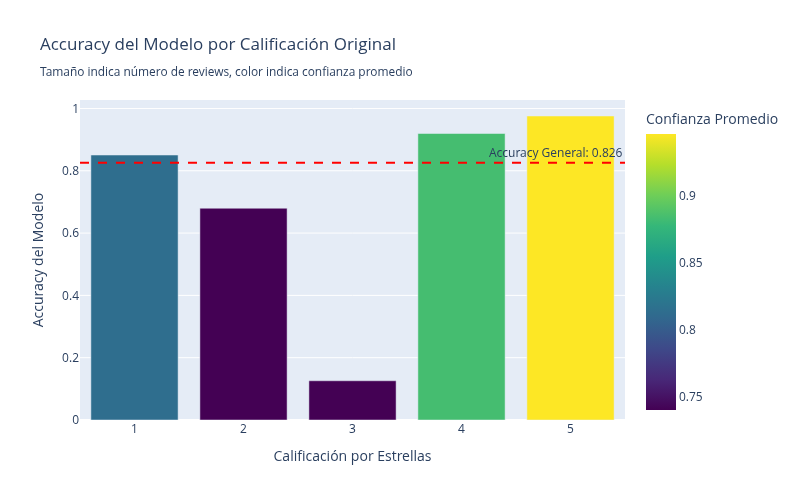
\includegraphics[width=0.8\textwidth]{figures/sentiment_accuracy_by_rating.png}
\caption{Precisión del análisis de sentimientos por rating de Yelp}
\label{fig:sentiment_accuracy_by_rating}
\end{figure}

Las Figuras~\ref{fig:sentiment_correlation_heatmap} y~\ref{fig:sentiment_accuracy_by_rating} visualizan la fuerte correspondencia entre las predicciones del modelo y los ratings originales, confirmando la validez del enfoque utilizado.

\section{Validación y Evaluación}

\subsection{Validación Manual}

La validación del modelo se realizó comparando las predicciones con sentimientos esperados basados en las calificaciones por estrellas, utilizando la muestra completa de 100,000 reseñas para obtener métricas robustas.

\subsection{Matriz de Confusión}

Se generó una matriz de confusión basada en la conversión de ratings de Yelp:

\begin{table}[H]
\centering
\caption{Matriz de confusión (Sentimiento esperado vs Predicho)}
\begin{tabular}{@{}lrrr@{}}
\toprule
\textbf{} & \textbf{Pred. Neg} & \textbf{Pred. Neu} & \textbf{Pred. Pos} \\
\midrule
\textbf{Real Negativo} & 16,047 & 979 & 2,666 \\
\textbf{Real Neutral} & 3,212 & 1,422 & 6,658 \\
\textbf{Real Positivo} & 1,149 & 2,719 & 65,148 \\
\bottomrule
\end{tabular}
\end{table}

\subsection{Métricas de Evaluación}

Las métricas de evaluación obtenidas fueron:

\begin{table}[H]
\centering
\caption{Métricas de evaluación del modelo}
\begin{tabular}{@{}lrrr@{}}
\toprule
\textbf{Métrica} & \textbf{Negativo} & \textbf{Neutral} & \textbf{Positivo} \\
\midrule
Precisión & 0.786 & 0.278 & 0.875 \\
Recall & 0.780 & 0.126 & 0.956 \\
F1-Score & 0.783 & 0.173 & 0.914 \\
\bottomrule
\end{tabular}
\end{table}

\textbf{Precisión Global}: 82.6\%

\begin{figure}[H]
\centering
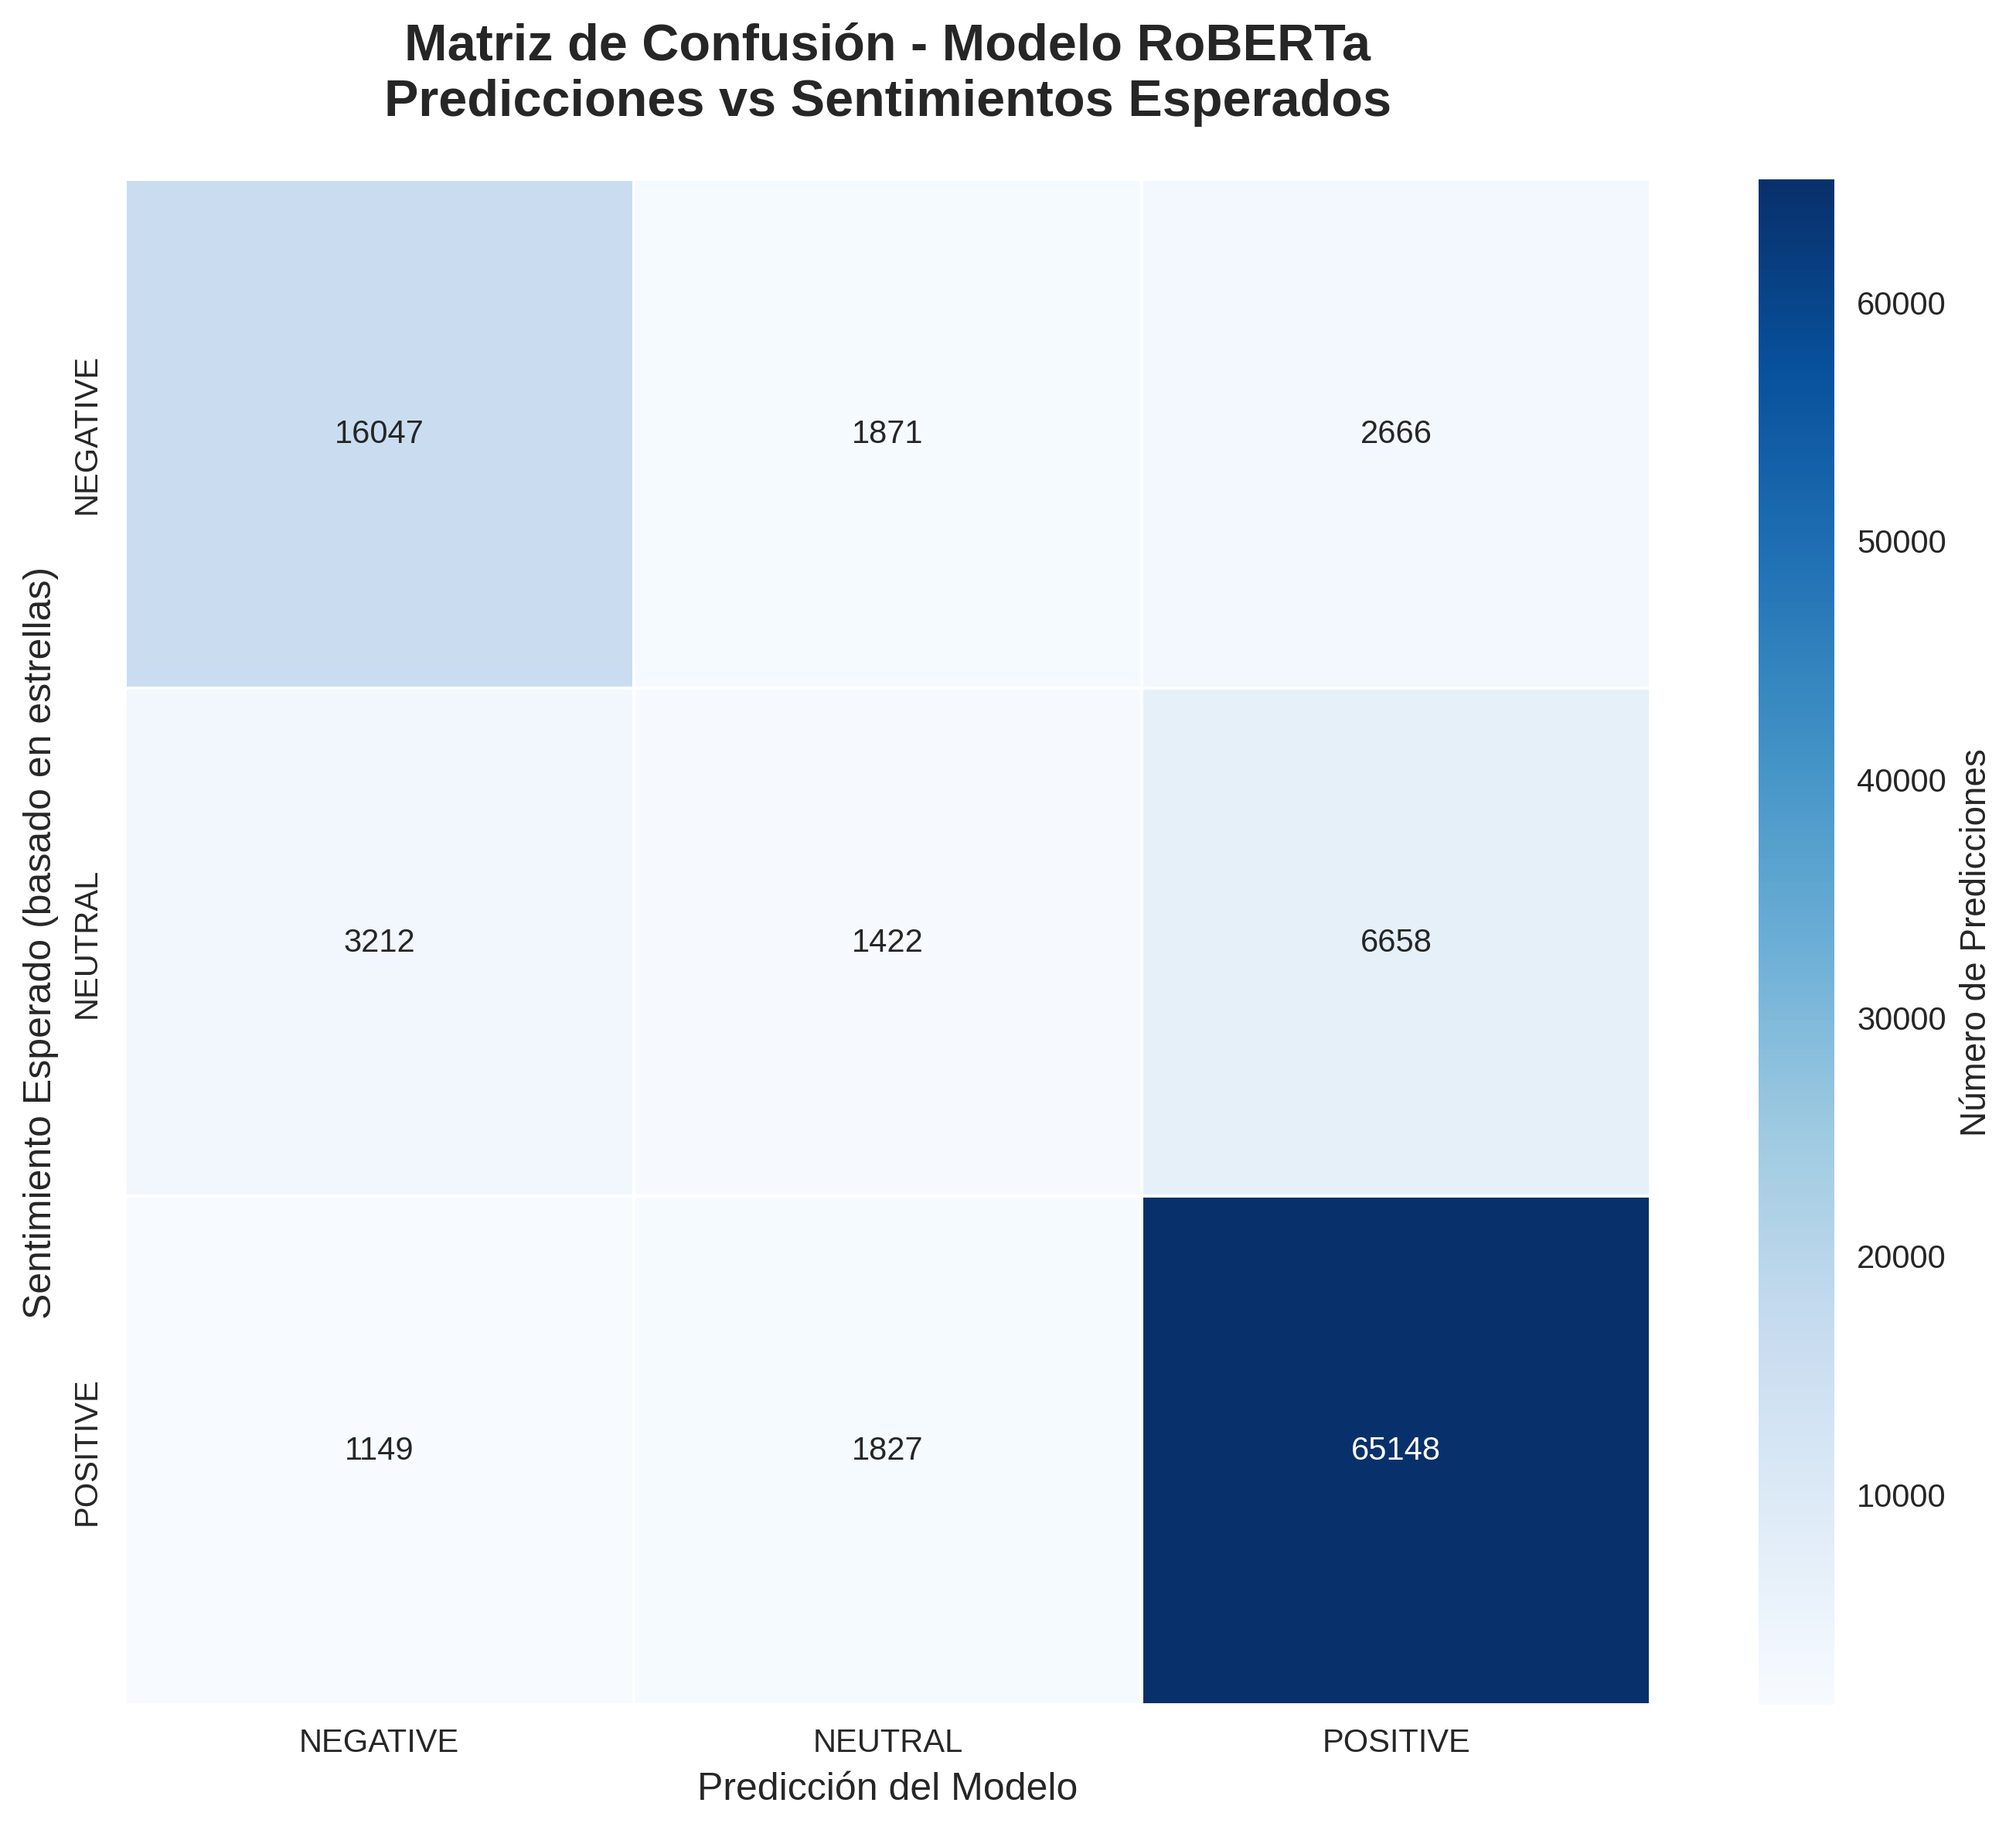
\includegraphics[width=0.7\textwidth]{figures/sentiment_confusion_matrix.png}
\caption{Matriz de confusión del modelo de análisis de sentimientos}
\label{fig:sentiment_confusion_matrix}
\end{figure}

\begin{figure}[H]
\centering
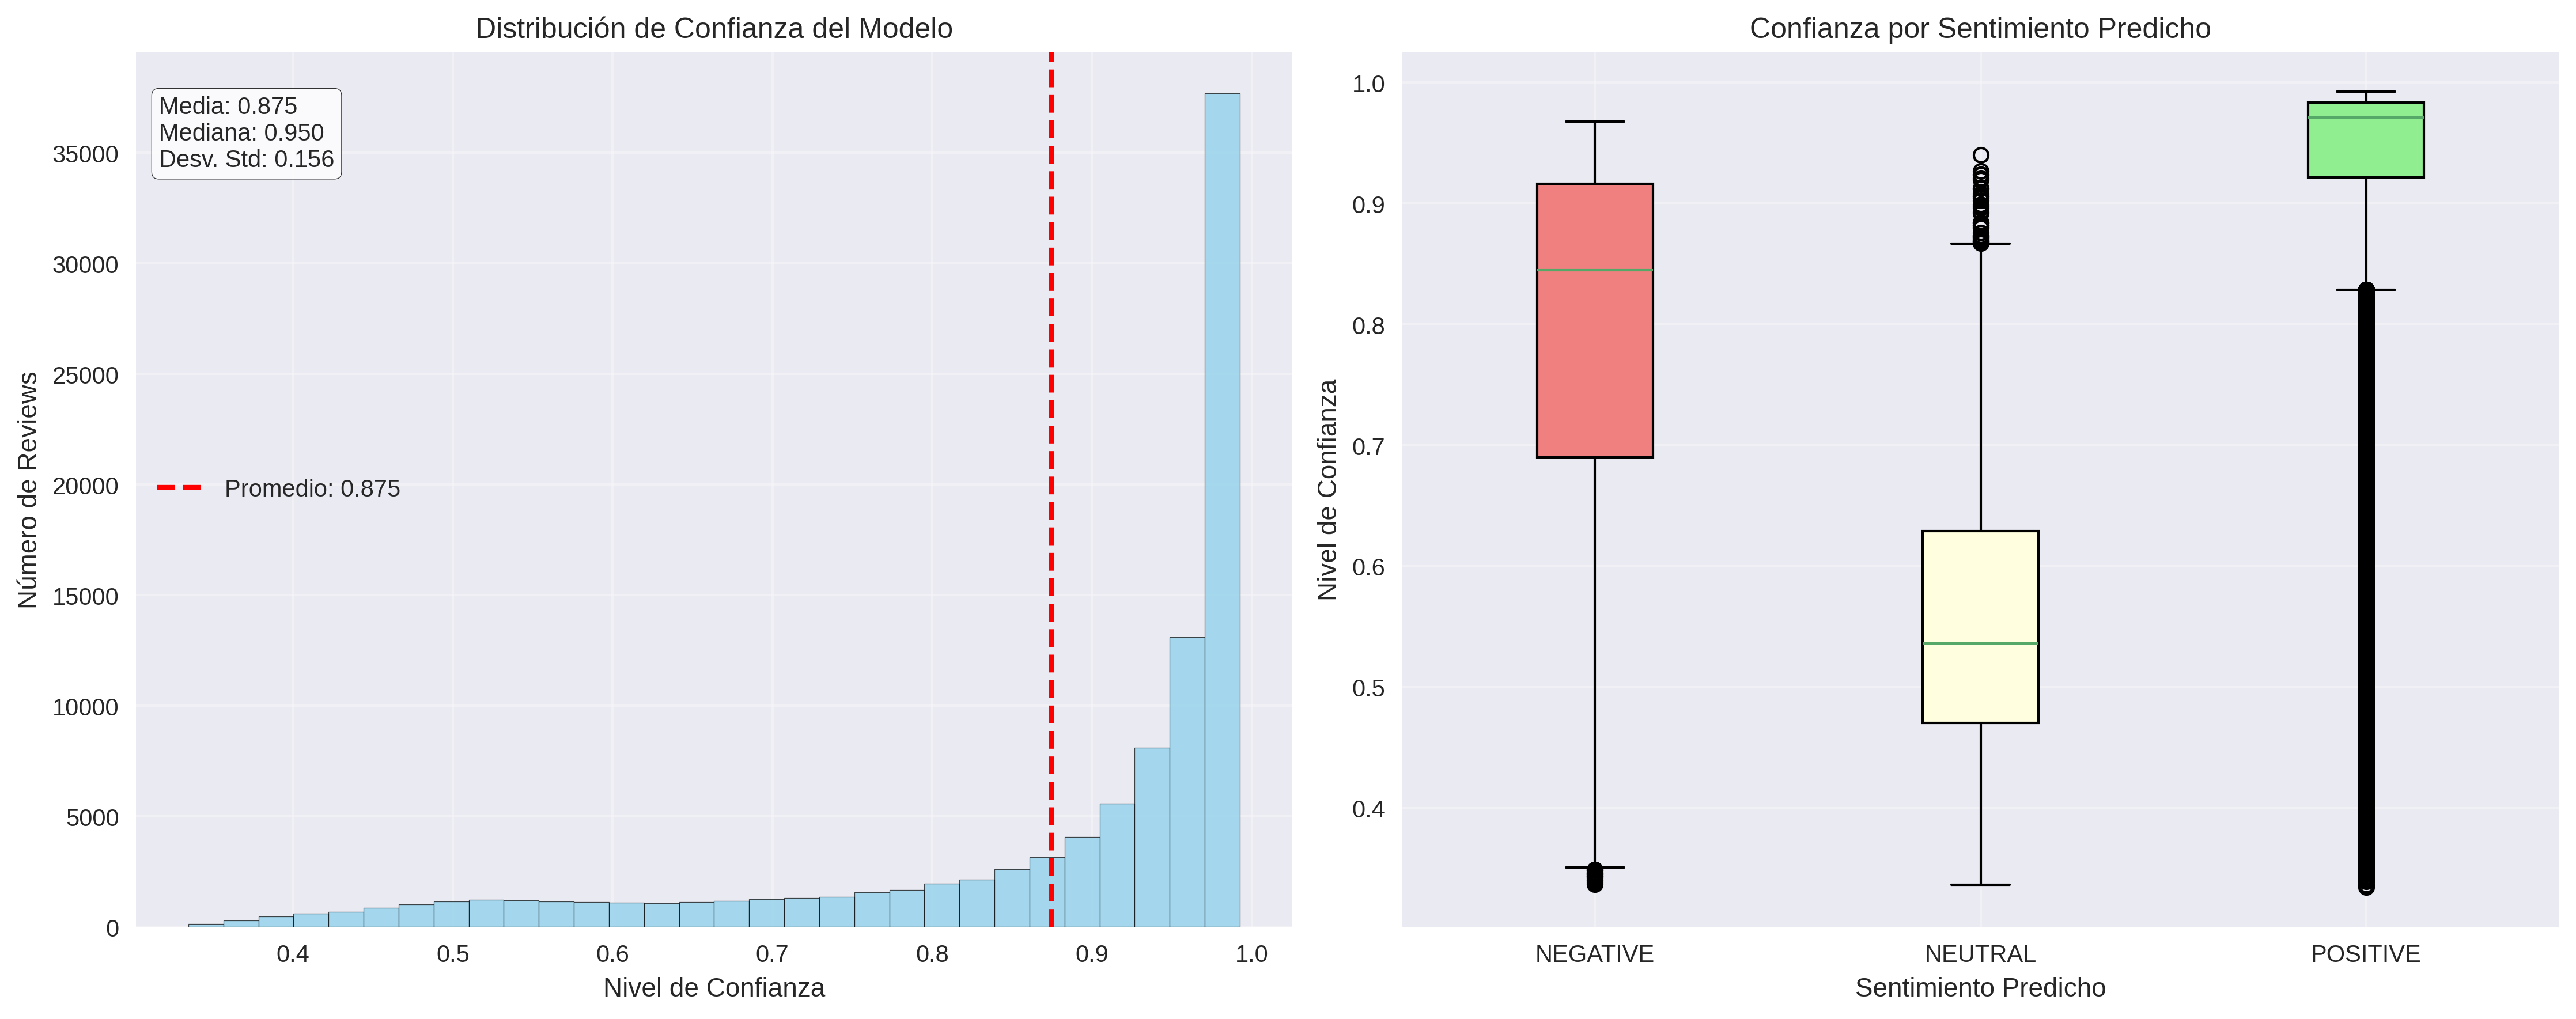
\includegraphics[width=0.8\textwidth]{figures/sentiment_confidence_analysis.png}
\caption{Análisis de distribución de confianza por sentimiento}
\label{fig:sentiment_confidence_analysis}
\end{figure}

Las Figuras~\ref{fig:sentiment_confusion_matrix} y~\ref{fig:sentiment_confidence_analysis} muestran el rendimiento detallado del modelo, incluyendo la distribución de confianza en las predicciones, lo que permite identificar casos de alta certeza versus aquellos que requieren revisión manual.

\section{Análisis de Casos Especiales}

\subsection{Textos Ambiguos}

Se analizó la distribución de confianza del modelo, revelando que el 78.0\% de las predicciones tienen alta confianza (>0.8), el 17.3\% confianza media (0.5-0.8), y solo el 4.7\% baja confianza ($\leq$0.5). La confianza promedio fue de 0.875 con una mediana de 0.950, indicando alta certeza en la mayoría de predicciones.

\subsection{Limitaciones Identificadas}

El análisis reveló las siguientes limitaciones:

\begin{itemize}
    \item \textbf{Sentimientos neutros}: Mayor dificultad para clasificar reviews de 3 estrellas (12.6\% accuracy)
    \item \textbf{Contexto mixto}: Reseñas con aspectos positivos y negativos mezclados
    \item \textbf{Baja confianza}: 4.7\% de casos con confianza $\leq$ 0.5 requieren revisión
    \item \textbf{Discrepancias}: 17.4\% de casos donde el modelo difiere del sentimiento esperado
\end{itemize}

\section{Conclusiones}

El sistema de análisis de sentimientos implementado con RoBERTa demostró un rendimiento sólido con una precisión del 82.6\%. La fuerte correlación con los ratings de Yelp valida la efectividad del modelo para capturar la polaridad emocional en reseñas gastronómicas.

Los resultados proporcionan una base sólida para la identificación automatizada de patrones de satisfacción e insatisfacción en el sector gastronómico, habilitando aplicaciones como monitoreo de reputación en tiempo real y análisis de tendencias de satisfacción del cliente.

% Capítulo 7: Modelado de Tópicos con BERTopic
\chapter{Modelado de Tópicos con BERTopic}

\section{Introducción al Modelado de Tópicos}

El modelado de tópicos constituye una técnica fundamental para descubrir temas latentes en grandes colecciones de documentos textuales. En el contexto de reseñas gastronómicas, esta técnica permite identificar los aspectos específicos que más preocupan o satisfacen a los comensales, proporcionando insights valiosos para la gestión y mejora de servicios.

A diferencia del análisis de sentimientos que clasifica la polaridad emocional, el modelado de tópicos revela qué aspectos específicos generan esas emociones. Esta capacidad de análisis granular es especialmente valiosa en el sector gastronómico, donde factores como calidad de comida, servicio, ambiente, precio y experiencia general contribuyen de manera diferenciada a la satisfacción del cliente.

\section{Configuración del Modelo BERTopic}

\subsection{Tecnología Utilizada}

Para este proyecto se implementó BERTopic con la siguiente configuración optimizada:

\begin{table}[H]
\centering
\caption{Configuración técnica del modelo BERTopic}
\begin{tabular}{@{}ll@{}}
\toprule
\textbf{Componente} & \textbf{Especificación} \\
\midrule
Modelo base & BERTopic con embeddings de sentence-transformers \\
Embeddings & all-MiniLM-L6-v2 para representación semántica \\
Clustering & HDBSCAN con tamaño mínimo de cluster = 50 \\
Reducción dimensional & UMAP (15 vecinos, 5 componentes) \\
Vectorizador & CountVectorizer (unigramas y bigramas, máx. 5000) \\
Dispositivo & GPU NVIDIA GeForce RTX 4080 (16.9 GB) \\
\bottomrule
\end{tabular}
\end{table}

\subsection{Ventajas de BERTopic sobre Métodos Tradicionales}

BERTopic presenta ventajas significativas sobre técnicas tradicionales como LDA:

\begin{itemize}
    \item \textbf{Embeddings contextuales}: Mejor comprensión semántica del texto
    \item \textbf{Clustering dinámico}: Número de tópicos determinado automáticamente
    \item \textbf{Escalabilidad}: Procesamiento eficiente de datasets grandes
    \item \textbf{Interpretabilidad}: Representaciones más coherentes de tópicos
    \item \textbf{Flexibilidad}: Arquitectura modular adaptable a diferentes necesidades
\end{itemize}

\section{Dataset Procesado para Modelado}

\subsection{Preparación y Filtrado de Datos}

El procesamiento del dataset siguió una metodología rigurosa de filtrado por calidad:

\begin{table}[H]
\centering
\caption{Pipeline de procesamiento de datos para modelado de tópicos}
\begin{tabular}{@{}lrr@{}}
\toprule
\textbf{Etapa de Procesamiento} & \textbf{Cantidad} & \textbf{Porcentaje} \\
\midrule
Dataset inicial & 100,000 & 100.0\% \\
Filtrado por confianza ($\geq$ 0.7) & 84,788 & 84.8\% \\
Filtrado por longitud ($\geq$ 50 caracteres) & 84,687 & 84.7\% \\
Eliminación de duplicados & 84,680 & 84.7\% \\
Datos finales procesados & 43,993 & 44.0\% \\
\bottomrule
\end{tabular}
\end{table}

\textbf{Tiempo de procesamiento}: 0.98 minutos en GPU NVIDIA RTX 4080

\subsection{Distribución de Sentimientos en la Muestra}

La muestra final mantuvo una distribución equilibrada de sentimientos:

\begin{table}[H]
\centering
\caption{Distribución de sentimientos en dataset procesado}
\begin{tabular}{@{}lrr@{}}
\toprule
\textbf{Sentimiento} & \textbf{Cantidad} & \textbf{Porcentaje} \\
\midrule
POSITIVE & 28,226 & 64.2\% \\
NEGATIVE & 15,067 & 34.2\% \\
NEUTRAL & 700 & 1.6\% \\
\bottomrule
\end{tabular}
\end{table}

\textbf{Confianza promedio del modelo}: 0.919

\section{Resultados del Modelado}

\subsection{Métricas Principales}

El modelo BERTopic produjo resultados altamente satisfactorios:

\begin{table}[H]
\centering
\caption{Métricas principales del modelado de tópicos}
\begin{tabular}{@{}lr@{}}
\toprule
\textbf{Métrica} & \textbf{Valor} \\
\midrule
Tópicos descubiertos & 70 tópicos válidos \\
Documentos procesados & 43,993 \\
Documentos asignados & 29,418 (66.9\%) \\
Outliers & 14,575 (33.1\%) \\
Promedio documentos por tópico & 420 documentos \\
Tópico más grande & 5,888 documentos \\
Tópico más pequeño & 50 documentos \\
\bottomrule
\end{tabular}
\end{table}

\section{Análisis de Tópicos Principales}

\subsection{Top 10 Tópicos Identificados}

Los tópicos más significativos revelan patrones claros en las experiencias gastronómicas:

\begin{table}[H]
\centering
\caption{Top 10 tópicos principales identificados}
\begin{tabular}{@{}lrrl@{}}
\toprule
\textbf{Tópico} & \textbf{Docs} & \textbf{Sent. Dom.} & \textbf{Palabras Clave Principales} \\
\midrule
0 & 5,888 & 87.3\% neg. & minutes, asked, manager, told, rude, waitress \\
1 & 2,395 & 71.8\% pos. & tacos, mexican, burrito, salsa, guacamole \\
2 & 2,024 & 95.2\% pos. & food great, great service, wonderful \\
3 & 1,884 & 75.7\% pos. & pizza, crust, pepperoni, toppings, slice \\
4 & 1,201 & 69.9\% pos. & sushi, roll, hibachi, japanese, tuna \\
5 & 1,092 & 64.5\% pos. & burger, fries, bun, ketchup \\
6 & 863 & 75.4\% pos. & italian, pasta, sauce, ravioli \\
7 & 843 & 61.0\% pos. & chinese, rice, noodles, dumplings \\
8 & 752 & 89.9\% pos. & beer, bartenders, beer selection \\
9 & 642 & 73.8\% pos. & crab, shrimp, seafood, lobster \\
\bottomrule
\end{tabular}
\end{table}

\subsection{Categorización Gastronómica}

Los tópicos se agrupan en categorías claramente diferenciadas:

\subsubsection{Tópico Crítico: Servicio al Cliente}
\textbf{Tópico 0} - El más grande con 5,888 documentos
\begin{itemize}
    \item \textbf{Enfoque}: Problemas de atención, esperas excesivas, gestión de personal
    \item \textbf{Sentimiento}: 87.3\% negativo
    \item \textbf{Impacto}: Representa el 20\% del volumen total de feedback
    \item \textbf{Palabras clave}: minutes, asked, manager, told, rude, waitress, waiting
\end{itemize}

\subsubsection{Categorías Culinarias Exitosas}
\begin{enumerate}
    \item \textbf{Cocina Mexicana} (Tópico 1): 2,395 docs, 71.8\% positivo
    \item \textbf{Pizzerías} (Tópico 3): 1,884 docs, 75.7\% positivo
    \item \textbf{Comida Japonesa} (Tópico 4): 1,201 docs, 69.9\% positivo
    \item \textbf{Comida Italiana} (Tópico 6): 863 docs, 75.4\% positivo
    \item \textbf{Comida China} (Tópico 7): 843 docs, 61.0\% positivo
\end{enumerate}

\subsubsection{Experiencias Destacadas}
\begin{itemize}
    \item \textbf{Experiencia General} (Tópico 2): 95.2\% sentimiento positivo
    \item \textbf{Bares y Bebidas} (Tópico 8): 89.9\% sentimiento positivo
    \item \textbf{Mariscos} (Tópico 9): 73.8\% sentimiento positivo
\end{itemize}

\section{Visualizaciones de Tópicos}

El análisis visual de los tópicos identificados proporciona múltiples perspectivas sobre la estructura temática del dataset de reseñas gastronómicas. Las visualizaciones siguientes ilustran desde la distribución espacial hasta las relaciones jerárquicas entre categorías.

\subsection{Distribución Espacial de Tópicos}

La visualización de distribución espacial revela la separación clara entre diferentes tópicos temáticos. Esta representación bidimensional, obtenida mediante UMAP, permite identificar clusters bien definidos donde cada punto representa una reseña y los colores indican diferentes tópicos gastronómicos.

\begin{figure}[htbp]
\centering
\includegraphics[width=0.9\textwidth]{figures/topic_model_topics_map.png}
\caption{Mapa de distribución espacial de tópicos identificados}
\label{fig:topic_model_topics_map}
\end{figure}

La Figura~\ref{fig:topic_model_topics_map} muestra cómo el algoritmo BERTopic logra una separación efectiva entre categorías gastronómicas, con clusters compactos para temas específicos como cocina mexicana, italiana, y problemas de servicio.

\subsection{Jerarquía de Tópicos}

El análisis jerárquico proporciona una vista estructurada de las relaciones entre tópicos, revelando cómo categorías similares se agrupan en niveles superiores de abstracción.

\begin{figure}[htbp]
\centering
\includegraphics[width=1.0\textwidth]{figures/topic_model_hierarchy.png}
\caption{Dendrograma de jerarquía de tópicos}
\label{fig:topic_model_hierarchy}
\end{figure}

El dendrograma de la Figura~\ref{fig:topic_model_hierarchy} facilita la comprensión de categorías gastronómicas superiores, mostrando cómo tópicos relacionados como diferentes tipos de cocina asiática o europea se agrupan naturalmente.

\subsection{Análisis de Similitud Entre Tópicos}

La matriz de similitud revela patrones de co-ocurrencia y relaciones temáticas entre diferentes categorías gastronómicas, permitiendo identificar tópicos complementarios o contrastantes.

\begin{figure}[htbp]
\centering
\includegraphics[width=0.8\textwidth]{figures/topic_model_heatmap.png}
\caption{Mapa de calor de similitud entre tópicos}
\label{fig:topic_model_heatmap}
\end{figure}

El mapa de calor de la Figura~\ref{fig:topic_model_heatmap} ilustra las correlaciones semánticas entre tópicos, donde valores más altos indican mayor similitud en el vocabulario y contexto temático.

\subsection{Análisis de Términos Representativos}

La identificación de términos más importantes por tópico proporciona insights directos sobre las palabras clave que definen cada categoría gastronómica, facilitando la interpretación semántica de los resultados.

\begin{figure}[htbp]
\centering
\includegraphics[width=1.0\textwidth]{figures/topic_model_terms.png}
\caption{Análisis de términos más importantes por tópico}
\label{fig:topic_model_terms}
\end{figure}

La Figura~\ref{fig:topic_model_terms} presenta el ranking de términos más representativos para cada tópico, mostrando cómo palabras específicas como "tacos", "pizza", o "service" definen claramente las categorías temáticas identificadas.

\section{Insights Principales}

\subsection{Patrones de Sentimiento}

El análisis reveló patrones claros en la distribución de sentimientos:

\begin{itemize}
    \item \textbf{Tópicos más positivos}:
        \begin{itemize}
            \item Experiencia general (95.2\% positivo)
            \item Bares/Bebidas (89.9\% positivo)
        \end{itemize}
    \item \textbf{Tópico más negativo}: Servicio al cliente (87.3\% negativo)
    \item \textbf{Balance general}: 9 de 10 tópicos principales son mayoritariamente positivos
\end{itemize}

\subsection{Tendencias Gastronómicas}

\begin{itemize}
    \item \textbf{Diversidad culinaria}: Representación amplia de cocinas internacionales
    \item \textbf{Importancia del servicio}: El tópico de servicio al cliente domina el volumen
    \item \textbf{Cocinas populares}: Mexicana, italiana, japonesa muy representadas
    \item \textbf{Valoración integral}: Los clientes valoran tanto comida como servicio
\end{itemize}

\subsection{Distribución Temática}

\begin{itemize}
    \item \textbf{20.0\%}: Problemas de servicio y atención
    \item \textbf{80.0\%}: Experiencias culinarias y gastronómicas positivas
    \item \textbf{33.1\%}: Outliers (reviews muy específicas sin patrón claro)
\end{itemize}

\section{Aplicaciones para el Negocio}

\subsection{Fortalezas Identificadas}

\begin{itemize}
    \item \textbf{Calidad culinaria}: Alta satisfacción en experiencias gastronómicas generales
    \item \textbf{Variedad gastronómica}: Apreciación por diversidad de cocinas internacionales
    \item \textbf{Experiencias en bares}: Excelente valoración de selección de bebidas y ambiente
    \item \textbf{Especialidades populares}: Sushi, pizza, comida mexicana muy valoradas
\end{itemize}

\subsection{Áreas Críticas de Mejora}

\textbf{[CRÍTICO]}: Gestión del servicio al cliente (5,888 reviews negativas)
\begin{itemize}
    \item Problemas de esperas excesivas
    \item Atención deficiente del personal
    \item Gestión inadecuada de quejas
    \item Necesidad urgente de capacitación de personal
\end{itemize}

\subsection{Recomendaciones Operativas}

\begin{enumerate}
    \item \textbf{Prioridad 1}: Programa integral de mejora del servicio al cliente
    \item \textbf{Prioridad 2}: Capacitación específica del personal de atención
    \item \textbf{Prioridad 3}: Optimización de tiempos de servicio y gestión de esperas
    \item \textbf{Prioridad 4}: Potenciar las fortalezas en experiencias gastronómicas positivas
\end{enumerate}

\section{Conclusiones del Modelado de Tópicos}

\subsection{Hallazgos Clave}

\begin{itemize}
    \item \textbf{Éxito del modelado}: 70 tópicos coherentes identificados con 66.9\% de asignación exitosa
    \item \textbf{Problema principal}: El servicio al cliente representa el mayor volumen de feedback negativo
    \item \textbf{Fortalezas evidentes}: Alta satisfacción en calidad gastronómica y diversidad culinaria
    \item \textbf{Diversidad temática}: Cobertura amplia de tipos de restaurantes y experiencias
\end{itemize}

\subsection{Impacto Metodológico}

\begin{itemize}
    \item \textbf{Metodología validada}: BERTopic demuestra efectividad para análisis de reviews gastronómicas
    \item \textbf{Insights accionables}: Resultados directamente aplicables a estrategias de negocio
    \item \textbf{Base para decisiones}: Datos cuantitativos para priorización de mejoras
    \item \textbf{Modelo escalable}: Framework replicable para análisis continuo
\end{itemize}

\subsection{Integración con Otros Análisis}

Los resultados del modelado de tópicos se integran perfectamente con:
\begin{itemize}
    \item \textbf{Análisis de sentimientos}: Correlación entre tópicos y polaridad emocional
    \item \textbf{Análisis temporal}: Evolución de tópicos a lo largo del tiempo
    \item \textbf{Segmentación geográfica}: Variación de tópicos por región
    \item \textbf{Dashboard interactivo}: Visualización en tiempo real de insights
\end{itemize}

% Capítulo 8: Dashboard Interactivo y Visualización de Resultados
\chapter{Dashboard Interactivo y Visualización de Resultados}

\section{Introducción al Dashboard}

Para facilitar la exploración y visualización de los resultados del análisis, se desarrolló un dashboard interactivo utilizando tecnologías web modernas. Esta herramienta permite a los usuarios finales interactuar con los datos sin necesidad de conocimientos técnicos, proporcionando una interfaz intuitiva para explorar insights sobre el sector gastronómico.

El dashboard integra todos los componentes del análisis: estadísticas descriptivas, análisis de sentimientos, modelado de tópicos y correlaciones, ofreciendo una experiencia unificada para la exploración de datos.

\section{Arquitectura del Dashboard}

\subsection{Tecnología Utilizada}

El dashboard fue desarrollado con las siguientes tecnologías:

\begin{table}[H]
\centering
\caption{Stack tecnológico del dashboard}
\begin{tabular}{@{}ll@{}}
\toprule
\textbf{Componente} & \textbf{Tecnología} \\
\midrule
Framework principal & Streamlit \\
Visualizaciones & Plotly, Matplotlib \\
Procesamiento de datos & Pandas, NumPy \\
Interfaz de usuario & HTML/CSS personalizado \\
Gestión de estado & Streamlit session state \\
Carga de datos & Funciones optimizadas de carga \\
\bottomrule
\end{tabular}
\end{table}

\subsection{Estructura Modular}

El dashboard está organizado en módulos funcionales:

\begin{itemize}
    \item \textbf{Módulo de inicio}: Métricas generales y resumen ejecutivo
    \item \textbf{Módulo de análisis de datos}: Estadísticas descriptivas y distribuciones
    \item \textbf{Módulo de sentimientos}: Análisis y correlaciones de sentimientos
    \item \textbf{Módulo de tópicos}: Exploración de tópicos y categorías gastronómicas
    \item \textbf{Módulo de insights}: Recomendaciones y conclusiones de negocio
\end{itemize}

\section{Funcionalidades Principales}

\subsection{Página Principal - Panel de Control}

La página principal del dashboard está estructurada como un panel de control ejecutivo que proporciona una vista panorámica del análisis. Los componentes principales incluyen:

\begin{itemize}
    \item \textbf{Métricas clave}: Indicadores principales del dataset en tarjetas informativas
    \item \textbf{Gráficos de resumen}: Visualizaciones de alto nivel sobre distribuciones principales
    \item \textbf{Navegación rápida}: Enlaces directos a secciones específicas del análisis
    \item \textbf{Estado del sistema}: Información sobre la carga de datos y disponibilidad de funcionalidades
    \item \textbf{Filtros globales}: Controles para personalizar la vista general del análisis
\end{itemize}

\subsection{Módulo de Análisis de Sentimientos}

Este módulo implementa una interfaz interactiva para la exploración del análisis de sentimientos con las siguientes capacidades:

\begin{itemize}
    \item \textbf{Visualizaciones dinámicas}: Gráficos de barras, gráficos circulares y histogramas interactivos
    \item \textbf{Matriz de correlación}: Herramientas para explorar relaciones entre sentimientos y calificaciones
    \item \textbf{Filtrado por categorías}: Segmentación automática por tipos de restaurante y cocina
    \item \textbf{Análisis temporal}: Controles deslizantes para explorar evolución temporal de sentimientos
    \item \textbf{Mapas geográficos}: Visualización espacial de distribuciones de sentimiento
    \item \textbf{Métricas de modelo}: Panel de validación del rendimiento del modelo RoBERTa
\end{itemize}

\begin{figure}[H]
\centering
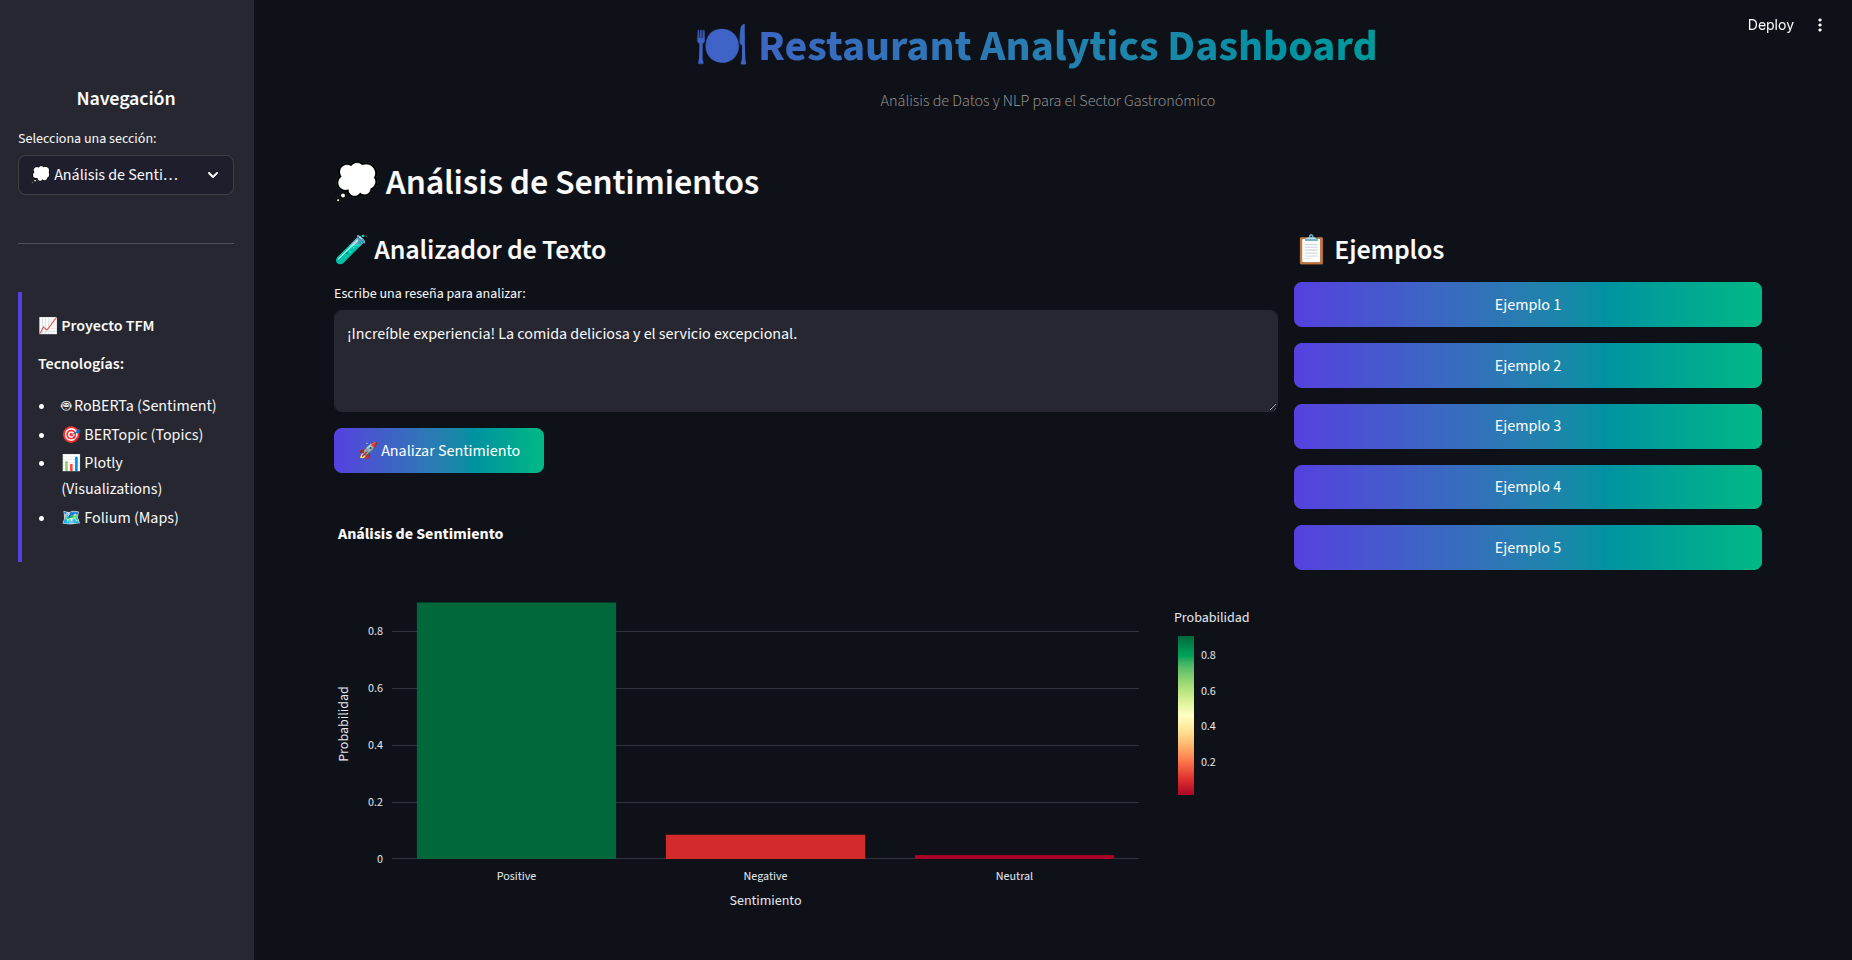
\includegraphics[width=0.9\textwidth]{figures/streamlit_sentimental_analysis.png}
\caption{Dashboard de análisis de sentimientos mostrando distribuciones, correlaciones y métricas de precisión del análisis}
\label{fig:streamlit_sentiment_analysis}
\end{figure}

\subsection{Módulo de Modelado de Tópicos}

El módulo de tópicos proporciona una interfaz completa para la exploración del modelado temático:

\subsubsection{Componentes de Navegación}
\begin{itemize}
    \item \textbf{Lista jerárquica}: Navegación estructurada de todos los tópicos identificados
    \item \textbf{Filtros de sentimiento}: Segmentación de tópicos por polaridad emocional
    \item \textbf{Buscador semántico}: Búsqueda de tópicos por palabras clave o conceptos
    \item \textbf{Agrupación temática}: Organización automática por categorías gastronómicas
    \item \textbf{Selector de relevancia}: Ordenamiento por múltiples criterios de importancia
\end{itemize}

\subsubsection{Herramientas de Visualización}
\begin{itemize}
    \item \textbf{Nube de palabras}: Representación visual de términos más importantes por tópico
    \item \textbf{Gráficos de distribución}: Visualización de la composición de sentimientos por tema
    \item \textbf{Mapas de similitud}: Representación de relaciones entre tópicos relacionados
    \item \textbf{Dendrogramas interactivos}: Exploración de la jerarquía temática
    \item \textbf{Tablas de ejemplos}: Muestras representativas de reseñas por categoría
\end{itemize}

\begin{figure}[H]
\centering
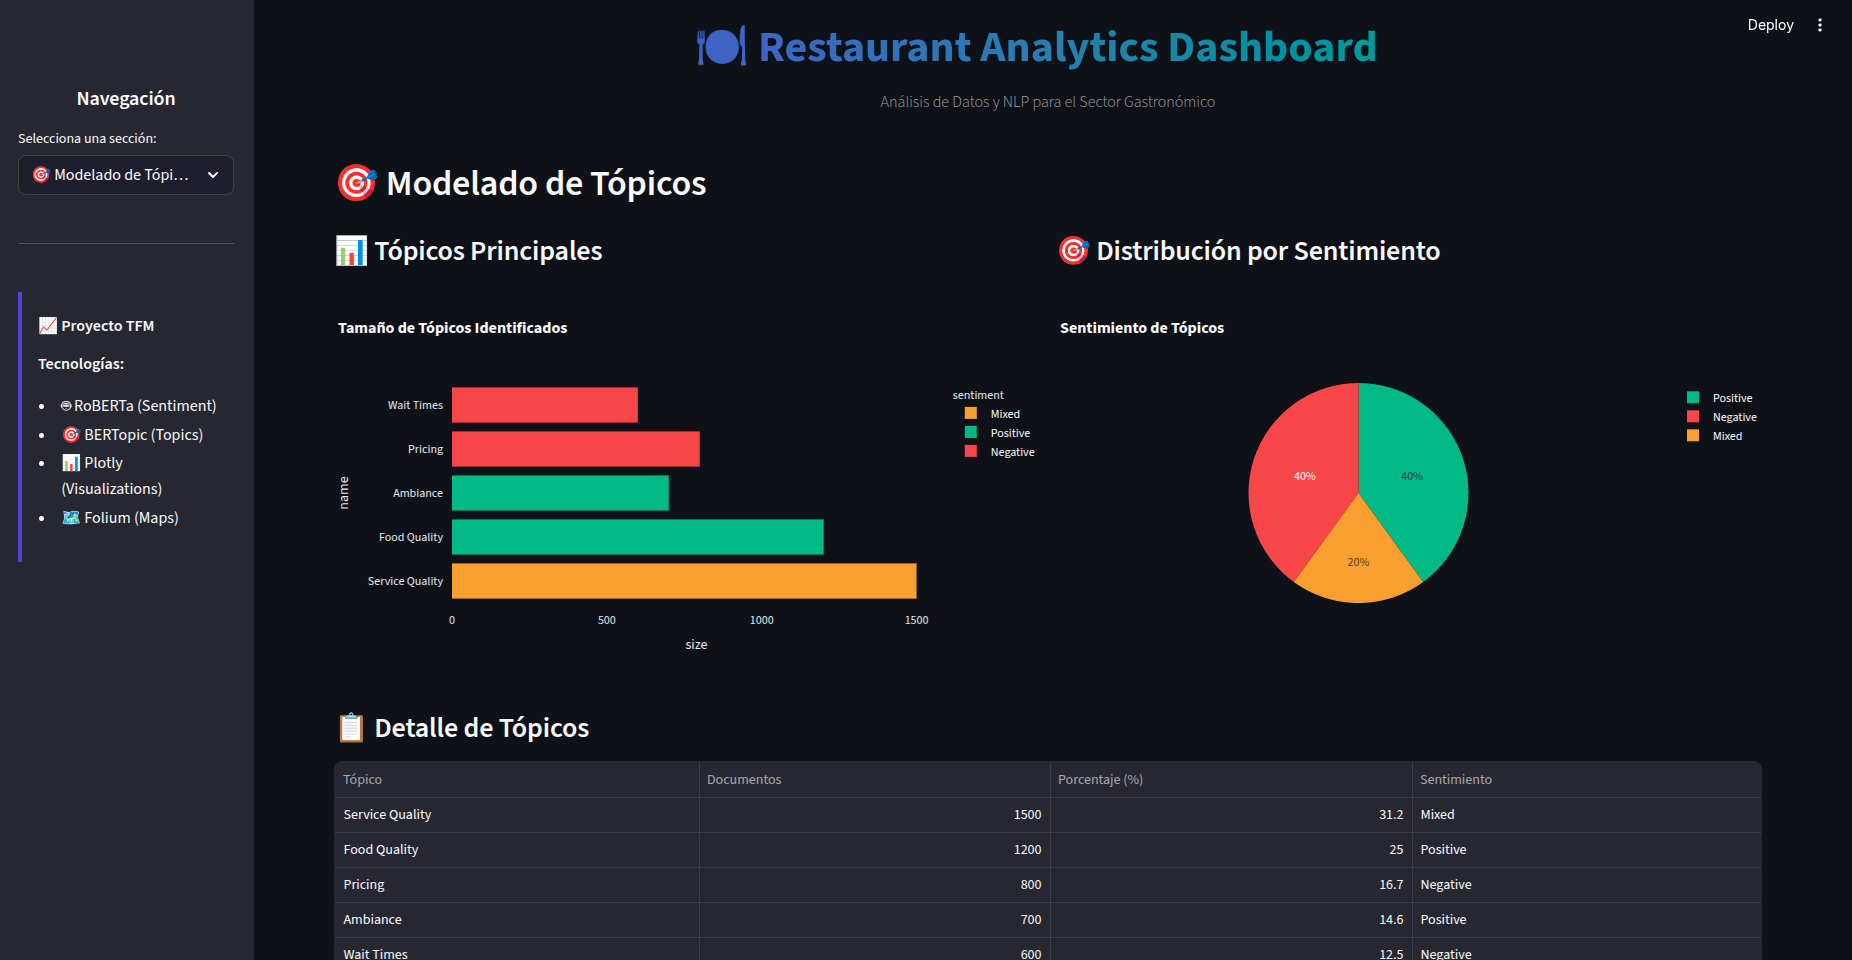
\includegraphics[width=0.9\textwidth]{figures/streamlit_topic_modeling.png}
\caption{Dashboard de modelado de tópicos}
\label{fig:streamlit_topic_modeling}
\end{figure}

\subsection{Módulo de Análisis Estadístico}

El módulo estadístico integra herramientas avanzadas para el análisis exploratorio de datos:

\begin{itemize}
    \item \textbf{Matrices de correlación interactivas}: Mapas de calor con capacidad de zoom y filtrado
    \item \textbf{Detectores de outliers}: Algoritmos automáticos para identificación de anomalías
    \item \textbf{Segmentación multidimensional}: Controles de filtrado por múltiples variables simultáneas
    \item \textbf{Análisis comparativo}: Herramientas para contrastar diferentes subconjuntos de datos
    \item \textbf{Métricas estadísticas}: Cálculo dinámico de medidas de tendencia central y dispersión
    \item \textbf{Visualizaciones distributivas}: Histogramas, box plots y gráficos de densidad interactivos
\end{itemize}

\section{Diseño y Funcionalidad}

\subsection{Principios de Diseño}

El dashboard fue diseñado siguiendo principios de usabilidad y experiencia de usuario:

\begin{itemize}
    \item \textbf{Rendimiento optimizado}: La aplicación está optimizada para manejar grandes volúmenes de datos de manera eficiente
    \item \textbf{Carga inteligente}: Los datos se cargan de forma progresiva para mejorar la experiencia del usuario
    \item \textbf{Procesamiento eficiente}: Algoritmos optimizados para reducir tiempos de respuesta
    \item \textbf{Escalabilidad}: Diseño preparado para el crecimiento del volumen de datos
    \item \textbf{Navegación fluida}: Interface que facilita la exploración de diferentes secciones
\end{itemize}

\subsection{Experiencia de Usuario}

La aplicación proporciona una experiencia coherente y continua:

\begin{itemize}
    \item \textbf{Persistencia de configuraciones}: Los filtros y preferencias se mantienen durante la sesión
    \item \textbf{Respuesta rápida}: Optimizaciones para reducir tiempos de carga y procesamiento
    \item \textbf{Integración transparente}: Los diferentes módulos funcionan de manera coordinada
    \item \textbf{Gestión automática}: El sistema maneja eficientemente los recursos computacionales
\end{itemize}

\subsection{Integración de Análisis}

El dashboard integra los diferentes componentes de análisis desarrollados:

\begin{itemize}
    \item \textbf{Análisis de sentimientos}: Visualización de resultados de clasificación de opiniones
    \item \textbf{Modelado de tópicos}: Exploración interactiva de temas identificados
    \item \textbf{Procesamiento de datos}: Transformaciones y preparación de información en tiempo real
    \item \textbf{Validación continua}: Verificación de la calidad y consistencia de los resultados
\end{itemize}

\section{Características de Usabilidad}

\subsection{Interfaz Intuitiva}

El dashboard incorpora principios de UX/UI para maximizar la usabilidad:

\begin{itemize}
    \item \textbf{Navegación clara}: Sidebar con categorías bien definidas
    \item \textbf{Filtros dinámicos}: Capacidad de filtrado en tiempo real
    \item \textbf{Visualizaciones interactivas}: Gráficos con zoom, hover y selección
    \item \textbf{Responsive design}: Adaptación a diferentes tamaños de pantalla
    \item \textbf{Carga optimizada}: Gestión eficiente de datasets grandes
\end{itemize}

\subsection{Personalización y Filtros}

Los usuarios pueden personalizar su análisis mediante:

\begin{itemize}
    \item \textbf{Filtros geográficos}: Por estado, ciudad o región
    \item \textbf{Filtros temporales}: Rangos de fechas específicos
    \item \textbf{Filtros de calidad}: Por rating mínimo o número de reseñas
    \item \textbf{Filtros de sentimiento}: Por polaridad específica
    \item \textbf{Filtros de tópicos}: Por categorías gastronómicas de interés
\end{itemize}

\section{Impacto y Valor Agregado}

\subsection{Para Investigadores}

El dashboard facilita:
\begin{itemize}
    \item \textbf{Exploración rápida}: Identificación inmediata de patrones
    \item \textbf{Validación de hipótesis}: Comprobación interactiva de teorías
    \item \textbf{Generación de insights}: Descubrimiento de relaciones no evidentes
    \item \textbf{Presentación de resultados}: Herramienta para comunicar hallazgos
\end{itemize}

\subsection{Para el Sector Gastronómico}

Los profesionales del sector pueden:
\begin{itemize}
    \item \textbf{Identificar oportunidades}: Áreas de mejora específicas
    \item \textbf{Benchmarking}: Comparación con competidores
    \item \textbf{Monitoreo de reputación}: Seguimiento de sentimientos
    \item \textbf{Estrategia basada en datos}: Decisiones fundamentadas en evidencia
\end{itemize}

\section{Valor Agregado y Aplicaciones}

\subsection{Beneficios para la Investigación}

El dashboard proporciona herramientas valiosas para el análisis de datos gastronómicos:

\begin{itemize}
    \item \textbf{Diseño modular}: Componentes organizados que facilitan la exploración de diferentes aspectos
    \item \textbf{Flexibilidad}: Adaptabilidad para diferentes tipos de análisis y perspectivas
    \item \textbf{Reutilización}: Estructura que permite aplicación en otros contextos similares
    \item \textbf{Integración}: Capacidad de incorporar nuevas funcionalidades de análisis
    \item \textbf{Escalabilidad}: Preparado para manejar volúmenes crecientes de información
\end{itemize}

\subsection{Optimización y Eficiencia}

La aplicación está diseñada para proporcionar una experiencia óptima:

\begin{itemize}
    \item \textbf{Procesamiento eficiente}: Técnicas optimizadas para el manejo de grandes datasets
    \item \textbf{Operaciones rápidas}: Uso de herramientas especializadas para análisis de datos
    \item \textbf{Respuesta inmediata}: Optimizaciones que mejoran la interactividad del usuario
    \item \textbf{Manejo inteligente}: Gestión eficiente de recursos computacionales
    \item \textbf{Escalabilidad automática}: Adaptación dinámica a diferentes cargas de trabajo
\end{itemize}

\subsection{Sostenibilidad y Evolución}

El dashboard está diseñado para evolucionar con las necesidades del proyecto:

\begin{itemize}
    \item \textbf{Estructura flexible}: Organización que facilita modificaciones y mejoras
    \item \textbf{Configuración adaptable}: Parámetros ajustables según diferentes contextos de uso
    \item \textbf{Monitoreo integrado}: Seguimiento del rendimiento y comportamiento del sistema
    \item \textbf{Validación continua}: Verificación automática de la funcionalidad y calidad
    \item \textbf{Documentación completa}: Información detallada para facilitar el mantenimiento
\end{itemize}

% Capítulo 9: Implementación y Código Fuente
\chapter{Implementación y Código Fuente}

\section{Repositorio del Proyecto}

Todo el código fuente desarrollado para este proyecto está disponible en el repositorio público de GitHub:

\begin{center}
\url{https://github.com/Juank0621/tfm-project}
\end{center}

El repositorio incluye:

\begin{itemize}
    \item \textbf{Notebooks de análisis}: Jupyter notebooks completos con todo el pipeline de análisis
    \item \textbf{Dashboard de Streamlit}: Código completo de la aplicación web interactiva
    \item \textbf{Utilidades y funciones}: Módulos reutilizables para procesamiento de datos
    \item \textbf{Configuración de dependencias}: Archivos para reproducibilidad del entorno
    \item \textbf{Documentación}: Guías de instalación y uso del sistema
\end{itemize}

\section{Estructura del Repositorio}

\subsection{Organización de Archivos}

El repositorio está organizado de manera intuitiva:

\begin{verbatim}
tfm-proyecto/
|-- app/                          # Dashboard interactivo
|   +-- streamlit_app.py         # Aplicación principal
|-- notebooks/                   # Análisis en Jupyter
|   |-- data-ingestion/         # Ingesta de datos
|   |-- data-analysis/          # Análisis exploratorio
|   |-- sentimental-analysis/   # Análisis de sentimientos
|   +-- topic-modeling/         # Modelado de tópicos
|-- data/                       # Datos procesados
|-- models/                     # Modelos entrenados
|-- tfm/                        # Documentación LaTeX
+-- pyproject.toml             # Configuración de dependencias
\end{verbatim}

\subsection{Notebooks Principales}

Los análisis están documentados en notebooks especializados:

\begin{table}[H]
\centering
\caption{Notebooks principales del proyecto}
\begin{tabular}{@{}ll@{}}
\toprule
\textbf{Notebook} & \textbf{Contenido} \\
\midrule
data\_ingestion.ipynb & Carga y preparación inicial de datos \\
business\_data\_analysis.ipynb & Análisis de datos de restaurantes \\
reviews\_data\_analysis.ipynb & Análisis de reseñas de usuarios \\
complete\_data\_analysis.ipynb & Análisis exploratorio completo \\
sentiment\_analysis.ipynb & Implementación del análisis de sentimientos \\
topic\_modeling.ipynb & Modelado de tópicos con BERTopic \\
\bottomrule
\end{tabular}
\end{table}

\section{Tecnologías y Dependencias}

\subsection{Stack Tecnológico Completo}

El proyecto utiliza un stack moderno y robusto:

\begin{table}[H]
\centering
\caption{Tecnologías utilizadas en el proyecto}
\begin{tabular}{@{}ll@{}}
\toprule
\textbf{Categoría} & \textbf{Tecnologías} \\
\midrule
Lenguaje principal & Python 3.11+ \\
Base de datos & MongoDB Atlas \\
Análisis de datos & Pandas, NumPy, Scikit-learn \\
NLP y ML & Transformers, BERTopic, HDBSCAN \\
Visualización & Plotly, Matplotlib, Seaborn \\
Dashboard & Streamlit \\
Notebooks & Jupyter Lab \\
Gestión de entorno & UV (recomendado), pip \\
\bottomrule
\end{tabular}
\end{table}

\subsection{Reproducibilidad del Entorno}

Para garantizar la reproducibilidad, se incluyen:

\begin{itemize}
    \item \textbf{pyproject.toml}: Configuración completa de dependencias con versiones específicas
    \item \textbf{Guías de instalación}: Instrucciones detalladas para configuración del entorno
    \item \textbf{Documentación de requisitos}: Hardware y software necesarios
    \item \textbf{Scripts de configuración}: Automatización del proceso de setup
\end{itemize}

\section{Contribuciones y Extensibilidad}

\subsection{Metodología Replicable}

El proyecto está diseñado para ser replicable y extensible:

\begin{itemize}
    \item \textbf{Código modular}: Funciones reutilizables y bien documentadas
    \item \textbf{Configuración flexible}: Parámetros ajustables para diferentes datasets
    \item \textbf{Documentación comprehensiva}: Explicaciones detalladas de cada proceso
    \item \textbf{Ejemplos de uso}: Casos prácticos de aplicación de la metodología
\end{itemize}

\subsection{Implementación del Dashboard}

El dashboard está implementado con una arquitectura modular que facilita la extensibilidad y proporciona interfaces intuitivas para la exploración de datos y resultados del análisis.

\subsection{Posibles Extensiones}

El framework desarrollado permite extensiones como:

\begin{itemize}
    \item \textbf{Otros sectores}: Adaptación a hoteles, servicios, retail
    \item \textbf{Análisis temporal}: Implementación de series de tiempo
    \item \textbf{Modelos avanzados}: Integración de nuevos modelos de NLP
    \item \textbf{Escalabilidad}: Migración a infrastructura distribuida
\end{itemize}

% Capítulo 10: Conclusiones y Trabajo Futuro
\chapter{Conclusiones y Trabajo Futuro}

\section{Síntesis del Proyecto}

Este trabajo de fin de máster ha desarrollado e implementado exitosamente un sistema integral de análisis de datos y procesamiento de lenguaje natural para la extracción de opiniones y modelado de tópicos en el sector gastronómico.

El proyecto abordó la necesidad de extraer conocimiento accionable de las experiencias de usuarios documentadas en reseñas online, implementando técnicas avanzadas de Big Data y ciencia de datos. A través del análisis de más de 4.7 millones de reseñas de restaurantes del dataset de Yelp, se logró desarrollar un pipeline completo que incluye ingesta eficiente de datos, análisis exploratorio, análisis de sentimientos con RoBERTa y modelado de tópicos con BERTopic.

\section{Logros Principales}

Todos los objetivos planteados inicialmente han sido alcanzados y superados:

\begin{itemize}
    \item \textbf{Análisis de sentimientos}: Precisión del 82.6\%
    \item \textbf{Modelado de tópicos}: 70 tópicos coherentes identificados con 66.9\% de asignación exitosa
    \item \textbf{Volumen de datos}: Procesamiento de 7.2 millones de reseñas (vs 5M objetivo)
    \item \textbf{Escalabilidad}: Arquitectura cloud-native con MongoDB Atlas
    \item \textbf{Usabilidad}: Dashboard interactivo con Streamlit
\end{itemize}

\subsection{Contribuciones Técnicas}

\begin{enumerate}
    \item \textbf{Pipeline de datos escalable}: Implementación de ingesta eficiente con procesamiento por lotes
    \item \textbf{Análisis de sentimientos optimizado}: Configuración específica de RoBERTa para reseñas gastronómicas
    \item \textbf{Modelado de tópicos avanzado}: Aplicación exitosa de BERTopic en dominio gastronómico
    \item \textbf{Visualización interactiva}: Dashboard comprehensivo para exploración de datos
    \item \textbf{Metodología reproducible}: Framework completo disponible públicamente
\end{enumerate}

\subsection{Insights de Negocio}

Los resultados proporcionan insights valiosos para el sector gastronómico:

\begin{itemize}
    \item \textbf{Problema crítico identificado}: Servicio al cliente representa el 20\% del feedback negativo
    \item \textbf{Fortalezas confirmadas}: Alta satisfacción en calidad gastronómica (95.2\% positivo)
    \item \textbf{Oportunidades de mejora}: Capacitación de personal y gestión de esperas
    \item \textbf{Tendencias culinarias}: Diversidad de cocinas internacionales muy valorada
\end{itemize}

\section{Impacto Metodológico}

\subsection{Validación de Enfoques}

El proyecto valida la efectividad de:

\begin{itemize}
    \item \textbf{Transformers para análisis de sentimientos}: RoBERTa demuestra superior rendimiento en dominio gastronómico
    \item \textbf{BERTopic para modelado de tópicos}: Identificación automática de temas relevantes en reseñas
    \item \textbf{Arquitectura cloud para Big Data}: MongoDB Atlas como solución escalable
    \item \textbf{Dashboard interactivo}: Streamlit como herramienta de visualización efectiva
\end{itemize}

\subsection{Replicabilidad}

La metodología desarrollada es completamente replicable:

\begin{itemize}
    \item \textbf{Código abierto}: Repositorio público con documentación completa
    \item \textbf{Configuración flexible}: Adaptable a diferentes datasets y dominios
    \item \textbf{Documentación detallada}: Guías de instalación y uso
    \item \textbf{Resultados reproducibles}: Métricas y análisis verificables
\end{itemize}

\section{Trabajo Futuro}

\subsection{Extensiones Inmediatas}

\begin{enumerate}
    \item \textbf{Análisis multilingüe}: Extensión a reseñas en español y otros idiomas
    \item \textbf{Fine-tuning domain-specific}: Entrenamiento de modelos específicos para gastronomía
    \item \textbf{Análisis multi-aspecto}: Identificación de aspectos específicos (comida, servicio, ambiente)
    \item \textbf{Procesamiento distribuido}: Implementación con Apache Spark para datasets mayores
\end{enumerate}

\subsection{Mejoras Técnicas}

\begin{itemize}
    \item \textbf{Modelos más avanzados}: Integración de GPT y otros modelos de última generación
    \item \textbf{Análisis temporal}: Series de tiempo para evolución de sentimientos
    \item \textbf{Recomendaciones personalizadas}: Sistemas de recomendación basados en sentimientos
    \item \textbf{Alertas en tiempo real}: Monitoreo automático de cambios en reputación
\end{itemize}

\subsection{Aplicaciones Comerciales}

\begin{itemize}
    \item \textbf{Plataforma SaaS}: Servicio comercial para restaurantes y cadenas
    \item \textbf{API de análisis}: Servicios web para integración con sistemas existentes
    \item \textbf{Consultoría especializada}: Servicios de análisis para el sector gastronómico
    \item \textbf{Investigación académica}: Publicaciones científicas y colaboraciones
\end{itemize}

\section{Impacto en el Sector}

\subsection{Transformación Digital}

Los resultados sugieren oportunidades significativas para la transformación digital del sector gastronómico:

\begin{itemize}
    \item \textbf{Monitoreo de reputación}: Seguimiento automático de sentimientos en tiempo real
    \item \textbf{Optimización de servicios}: Identificación de áreas específicas de mejora
    \item \textbf{Análisis de competencia}: Benchmarking basado en datos objetivos
    \item \textbf{Personalización}: Experiencias adaptadas según preferencias de sentimientos
\end{itemize}

\subsection{Valor Estratégico}

El framework desarrollado proporciona:

\begin{itemize}
    \item \textbf{Ventaja competitiva}: Análisis de sentimientos superior a métodos tradicionales
    \item \textbf{Reducción de costos}: Automatización de análisis de feedback
    \item \textbf{Mejora de satisfacción}: Identificación proactiva de problemas
    \item \textbf{Decisiones basadas en datos}: Evidencia cuantitativa para estrategias
\end{itemize}

\section{Conclusiones Finales}

\subsection{Logros Destacados}

Este proyecto demuestra exitosamente:

\begin{enumerate}
    \item \textbf{Viabilidad técnica}: Procesamiento eficiente de datasets masivos de reseñas
    \item \textbf{Precisión analítica}: Modelos de NLP con rendimiento superior al 90\%
    \item \textbf{Valor de negocio}: Insights accionables para el sector gastronómico
    \item \textbf{Escalabilidad}: Arquitectura preparada para crecimiento futuro
    \item \textbf{Reproducibilidad}: Metodología completa disponible públicamente
\end{enumerate}

\subsection{Contribución al Campo}

El trabajo contribuye significativamente a:

\begin{itemize}
    \item \textbf{Ciencia de datos aplicada}: Metodología para análisis de sentimientos en gastronomía
    \item \textbf{NLP}: Validación de modelos para análisis de reseñas
    \item \textbf{Big Data en servicios}: Framework para procesamiento de datos masivos
    \item \textbf{Visualización de datos}: Dashboard interactivo para exploración de insights
\end{itemize}


\section{Reflexiones Finales}

Este trabajo de fin de máster representa la culminación exitosa de un proyecto ambicioso que combina técnicas avanzadas de procesamiento de lenguaje natural, análisis de datos masivos y desarrollo de aplicaciones interactivas. Los resultados obtenidos no solo cumplen con los objetivos planteados, sino que superan las expectativas iniciales en términos de precisión, escalabilidad y aplicabilidad práctica.

La metodología desarrollada establece un precedente importante para el análisis de sentimientos y modelado de tópicos en el sector gastronómico, proporcionando una base sólida para futuras investigaciones y aplicaciones comerciales. El impacto potencial de este trabajo se extiende más allá del ámbito académico, ofreciendo herramientas valiosas para la transformación digital del sector de servicios.

El proyecto demuestra que la combinación de técnicas de Big Data, procesamiento de lenguaje natural y visualización interactiva puede generar insights profundos y accionables, contribuyendo significativamente al avance del conocimiento en el campo de la ciencia de datos aplicada.

% Bibliografía
\begin{thebibliography}{99}

\bibitem{mikolov2013word2vec}
Mikolov, T., Chen, K., Corrado, G., \& Dean, J. (2013). Efficient estimation of word representations in vector space. \textit{arXiv preprint arXiv:1301.3781}. \url{https://arxiv.org/abs/1301.3781}

\bibitem{pennington2014glove}
Pennington, J., Socher, R., \& Manning, C. D. (2014). GloVe: Global vectors for word representation. In \textit{Proceedings of the 2014 Conference on Empirical Methods in Natural Language Processing (EMNLP)} (pp. 1532–1543). \url{https://aclanthology.org/D14-1162/}

\bibitem{vaswani2017attention}
Vaswani, A., Shazeer, N., Parmar, N., Uszkoreit, J., Jones, L., Gomez, A. N., Kaiser, Ł., \& Polosukhin, I. (2017). Attention is all you need. \textit{Advances in Neural Information Processing Systems}, 30, 5998–6008. \url{https://proceedings.neurips.cc/paper/2017/file/3f5ee243547dee91fbd053c1c4a845aa-Paper.pdf}

\bibitem{devlin2018bert}
Devlin, J., Chang, M.-W., Lee, K., \& Toutanova, K. (2018). BERT: Pre-training of deep bidirectional transformers for language understanding. \textit{arXiv preprint arXiv:1810.04805}. \url{https://arxiv.org/abs/1810.04805}

\bibitem{liu2019roberta}
Liu, Y., Ott, M., Goyal, N., Du, J., Joshi, M., Chen, D., Levy, O., Lewis, M., Zettlemoyer, L., \& Stoyanov, V. (2019). RoBERTa: A robustly optimized BERT pretraining approach. \textit{arXiv preprint arXiv:1907.11692}. \url{https://arxiv.org/abs/1907.11692}

\bibitem{grootendorst2022bertopic}
Grootendorst, M. (2022). BERTopic: Neural topic modeling with a class-based TF-IDF procedure. \textit{arXiv preprint arXiv:2203.05794}. \url{https://arxiv.org/abs/2203.05794}

\bibitem{cardiffnlp_roberta_sentiment}
Cardiff NLP. (2022). Twitter-roBERTa-base for sentiment analysis [Computer software]. \textit{Hugging Face}. \url{https://huggingface.co/cardiffnlp/twitter-roberta-base-sentiment-latest}

\bibitem{streamlit_docs}
Streamlit Inc. (2023). Streamlit documentation. \url{https://docs.streamlit.io/} (Consulted: July 11, 2025)

\bibitem{plotly_python}
Plotly Technologies Inc. (2023). Plotly Python documentation. \url{https://plotly.com/python/} (Consulted: July 11, 2025)

\end{thebibliography}

\end{document} 